%
% Chapter 2
%
% Systems vaccinology-style HIRD paper.

% The one central and memorable contribution of the paper.
\chapter{Transcriptomic response to Pandemrix vaccine}
\label{ch:hird_DGE}

\textit{
    The work presented in this chapter is a collaboration between 
    the Wellcome Sanger Institute,
    King's College London, 
    the Francis Crick Institute,
    and the Biomedical Research Centre at Guy's and St Thomas' Hospital and King's College London.
    I would like to thank 
    Adrian Hayday, for kindly extending the opportunity to collaborate on the HIRD cohort;
    Efstathios Theodoridis, for performing the RNA and DNA extractions;
    Sean O'Farrel and Anna Lorenc, for providing the HIRD clinical, FACS, and antibody titre data, and for providing advice on the data formats;
    and the Wellcome Sanger Institute Sample Management and Pipelines teams, for performing the RNA-seq library preparation and sequencing, and the array genotyping.
}

\section{Introduction}

\subsection{Influenza}

Influenza is an infectious respiratory disease caused by the influenza virus family (\textit{Orthomyxoviridae}) in a variety of vertebrate hosts.
% bresee2018InactivatedInfluenzaVaccines
% Asymptomatic influenza infections are likely common, and may account for greater than 30% of all influenza infections,62, 63, 64, 65, 66, 67 although estimates have varied considerably depending on methods used to confirm influenza infection and study design.68 Asymptomatically infected persons can shed detectable influenza virus and may transmit influenza to others.69
Of the four virus types (A, B, C, D) defined by antigenic specificity of the viral nucleoprotein,
human infections are primarily caused by influenza A and influenza B.
Each year, seasonal epidemics result in \textapprox{1} billion infections and \numrange{300000}{500000} deaths worldwide.
Peak seasonality is defined by low humidity, low temperature, and other climate factors.
Risk factors for severe illness and death include extremes of age (infants \SI{<1}{\year}, elderly \SI{>65}{\year}), pregnancy, obesity, chronic illness, and host genetics (e.g. mutations in \gene{IFITM3} and \gene{IRF7}) \autocite{krammer2018Influenza,dhakal2019HostFactorsImpact}.

Influenza viruses are enveloped viruses with a negative-sense single-stranded RNA genome divided into segments (eight segments in influenza A and B), each encoding one or more viral proteins.
% Negative-sense (3′-to-5′) viral RNA is complementary to the viral mRNA, thus a positive-sense RNA must be produced by an RNA-dependent RNA polymerase from it prior to translation.
Two glycoproteins occurring on the surface of the viral envelope are the main antigens targeted by the host immune system.
\Gls{HA}, with its characteristic head-stalk structure, facilitates viral entry by binding sialic acid-containing surface receptors on host cells.
\Gls{NA} facilitates viral release, cleaving sialic acids to prevent newly-synthesised viruses aggregating to each other---viral proteins can be sialylated post-translation---and to the dying host cell in the final stages of the viral life cycle.
The gradual accumulation of mutations in these surface protein genes is known as antigenic drift,
and can lead to evasion of antibody-mediated immunity acquired during previous exposures.
As the virus type with the greatest prevalence, host range, and genetic diversity,
influenza A is classified into a number of subtypes based on the antigenic properties of its \gls{HA} and \gls{NA}.
% Defined by double immunodiffusion (DID) reactions
At least 18 \gls{HA} subtypes and 11 \gls{NA} subtypes exist \autocite{krammer2019HumanAntibodyResponse}.
Although these \gls{HA} and \gls{NA} subtypes are all antigenically-dissimilar, 
there can still be cross-reactivity between subtypes, and considerable antigenic drift within subtypes \autocite{worldhealthorganization1980RevisionSystemNomenclature}.
%
% krammer2019HumanAntibodyResponse
% The introduction of a new pandemic virus strain, as occurred in 2009 with the pandemic H1N1 virus, poses an extraordinary challenge to the immune system. Before 2009, humans had been widely exposed to seasonal H1N1 viruses. The HA expressed by these seasonal viruses is markedly different from the HA expressed by the 2009 pandemic H1N1 virus, although they are of the same HA subtype. However, the differences are not equally distributed within the H1 HA protein. The head domains of seasonal and pandemic H1 proteins differ greatly (having ~68% amino acid identity), whereas the stalk domains are highly conserved (having ~88% amino acid identity). In addition, some specific epitopes of the head domain are shared between seasonal and pandemic H1 proteins. Therefore, first exposure to the 2009 pandemic H1N1 virus triggered a recall response of those B cells that recognized the conserved, shared epitopes, which led to a significant response to the HA stalk (Box 1). This response was observed after both natural infection and vaccination43,113,132–135. It has been hypothesized that this increase in the production of cross-reactive antibodies led to the disappearance of seasonal H1N1 viruses after the emergence of the 2009 pandemic H1N1 virus43.
%
Influenza B viruses are less diverse, classified into two antigenically-distinct lineages: Victoria-like and Yamagata-like \autocite{krammer2018Influenza}.

On occasion, reassortment of genome segments between viruses infecting the same cell can quickly generate new strains (antigenic shift).
Antigenic shifts are associated with pandemics due to lack of pre-existing population immunity \autocite{krammer2018Influenza}.
% Pandemic severity depends on viral virulence.
Pandemics have occurred four times in modern history: 1918 (\enquote{Spanish}), 1957 (\enquote{Asian}), 1968 (\enquote{Hong Kong}), and 2009 (\enquote{swine}).
Each was caused by influenza A, involving either reassortment of human and animal strains or zoonotic transmission of animal strains \autocite{short2018BackFutureLessons}.
% Conclusive evidence that protective influenza virus-specific antibody responses are indeed long-lived came from the 2009 influenza pandemic. 
% Here, elderly people who were exposed to the 1918 influenza virus (or its immediate descendant), 60–90 years prior to the pandemic of 2009, were protected from infection and severe disease, as they maintained the antibody response that cross-reacted with the 2009 pandemic strain (Yu et al., 2008; Hancock et al., 2009; Ikonen et al., 2010; Reed and Katz, 2010).
%
For instance, the 2009 pandemic was due to an influenza A strain with \gls{HA} subtype 1 and \gls{NA} subtype 1 gene segments of swine origin \autocite{garten2009AntigenicGeneticCharacteristics}: A(H1N1)pdm09%
\footnote{
    The suffix \enquote{pdm09} distinguishes the 2009 pandemic strain from the circulating seasonal A(H1N1) strains at that time \autocite{worldhealthorganization2011StandardizationTerminologyPandemic}.
}.
Pandemic strains tend to enter seasonal circulation post-outbreak, potentially replacing previously-circulating strains;
A(H1N1)pdm09-like strains are now the predominant seasonal A(H1N1) strain \autocite{krammer2018Influenza}.
% See:
% Mechanisms of replacement of circulating viruses by seasonal and pandemic influenza A viruses
% PMID: 27569827 DOI: 10.1016/j.ijid.2016.08.012
%
% Why Do Influenza Virus Subtypes Die Out? A Hypothesis
% DOI: 10.1128/mBio.00150-11

\subsection{Seasonal influenza vaccines}

Vaccination is the primary method for prevention and control of influenza.
Antigenic drift and decline of vaccine-induced immunity over time means annual vaccination is recommended.
Seasonal vaccines are multivalent, usually formulated against three (trivalent) or four (quadrivalent) influenza strains anticipated to circulate in upcoming influenza seasons.
The \gls{WHO}-run Global Influenza Surveillance Response System (GISRS) makes recommendations on the most representative strains for the Northern and Southern hemispheres each year, about six months before the start of the respective seasons.

% bresee2018InactivatedInfluenzaVaccines
% Inactivated whole virus vaccines are no longer in use, as split ones are still immunogenic, but less reactogenic.
There are three classes of licensed vaccines against seasonal influenza: \glspl{IIV}, \glspl{LAIV}, and recombinant \gls{HA} vaccines \autocite{houser2015InfluenzaVaccinesChallenges,krammer2019HumanAntibodyResponse}.
\Glspl{IIV} can be split virion, containing virions disrupted with detergent, or subunit, containing further purified \gls{HA} protein.
\Glspl{LAIV} contain low-virulence, cold-adapted viruses that replicate well only in the cool upper respiratory tract.
Recombinant \gls{HA} vaccines contain purified recombinant \gls{HA} expressed in insect cell lines rather than relying on traditional viral propagation in embryonated chicken eggs; cell-based \glspl{IIV} are also available. 
Cell-based vaccines are faster to manufacture in pandemic situations, not dependent on egg supply, and avoids egg-adaptation: mismatches between vaccine and circulating strains caused by adaptation to growth in eggs.

Licensed seasonal vaccines are effective and well-tolerated in healthy adults, but particular subclasses of vaccine are recommended for different demographics \autocite{bresee2018InactivatedInfluenzaVaccines,luke2018InfluenzaVaccineLive,poland2018PersonalizedVaccinologyReview,ramsay2020InfluenzaGreenBook}.
\glspl{LAIV} are delivered via nasal spray and are more effective than \glspl{IIV} at mitigating transmission. 
They are recommended for children---the major drivers of transmission due to high viral loads and prolonged shedding \autocite{krammer2018Influenza,bresee2018InactivatedInfluenzaVaccines}---but are contraindicated in young children \SI{<2}{\year} due to increased risk of wheezing, and also in immunocompromised individuals.
Trials suggest \gls{LAIV} has superior efficacy compared to \glspl{IIV} in children.
High-dose and adjuvanted \gls{IIV} vaccines are recommended to enhance immunogenicity in the elderly.
% Generally, adjuvants improve vaccine responses but may increase reactogenicity.
Cell-based and egg-free vaccines are suitable for people with egg allergies.
No vaccines are licensed for use in infants \SI{<6}{\month}, but passive immunity can be conferred through vaccinating the mother.

Point estimates of seasonal vaccine efficacy range from \SIrange{50}{90}{\percent} in healthy adults in controlled trials.
% TODO: add efficacy definition as footnote
Real-world effectiveness can be as low as \SI{10}{\percent}, depending greatly on vaccine class, choice of endpoint, the match between vaccine and circulating strains, and various host factors
% (e.g. age, sex, immune history, pregnancy, obesity, microbiome, genetics)
\autocite{dhakal2019HostFactorsImpact,zimmermann2019FactorsThatInfluence}.
In general, efficacy is comparable or better in children versus young adults, and lowest in the elderly due to immunosenescence.
Females mount higher antibody responses than males to \glspl{IIV} regardless of age, potentially mediated by sex steroid levels \autocite{furman2014SystemsAnalysisSex,dhakal2019HostFactorsImpact}.
Immune history has a major impact on vaccine response due to immune memory.
Adults primed by past exposures to seasonal influenza strains have qualitatively different responses to unprimed adults or influenza-naive children.
For example, 
influenza-naive children mount much higher serum antibody responses to seasonal \gls{LAIV} than primed adults \autocite{luke2018InfluenzaVaccineLive};
% TODO: add some elaboration as to why
and antibody responses to \gls{IIV} peak later in unprimed individuals, requiring two doses to generate optimal concentrations \autocite{bresee2018InactivatedInfluenzaVaccines}.
Immune history also affects response via antigenic seniority (a.k.a. immune imprinting), 
where the antibody response is biased towards recall against strains encountered in early childhood
over generation of a \textit{de novo} response.
This is beneficial if strains with the same epitopes come back into circulation, 
% Indeed, the decreased susceptibility of the elderly population to both the 1918 and the 2009 H1N1 pandemics has been attributed to cross-protection from antibodies generated to strains encountered in childhood [7,40–42].
and harmful against strains still similar enough to trigger immune memory, but with drifted epitopes \autocite{henry2018OriginalAntigenicSin,dhakal2019HostFactorsImpact}.
% TODO: how do drifted epitopes trigger immune memory?
% OAS may be more prominent for repeated flu infection rather than repeated vaccination https://www.jimmunol.org/content/183/5/3294
% Also see "Original antigenic sin: A comprehensive review" https://doi.org/10.1016/j.jaut.2017.04.008
% TODO: add pregnancy, obesity, microbiome
Finally, host genetic variation in cytokine genes, immunoglobulin genes, and the \gls{HLA} region are associated with antibody responses---reviewed in \cref{subsec:hird_reQTL_intro_geneticFactorsFluVaccine}.

\subsection{Quantifying immune response to influenza vaccines}

The efficacy of \glspl{IIV} is mostly mediated by induction of strain-specific anti-\gls{HA} antibodies,
although other antibodies (e.g. anti-\gls{NA}) may also contribute in the case of non-purified vaccines.
\Glspl{ASC} in peripheral blood peak around one week after vaccination, and serum antibodies peak around two to four weeks after vaccination.
Antibody-mediated protection may last up to a year in healthy adults \autocite{bresee2018InactivatedInfluenzaVaccines,davis2020InfluenzaVaccineInduced}.
The immunodominance of the \gls{HA} head over the stalk means most anti-\gls{HA} antibodies have epitopes in the head domain.
Unsurprisingly, the resulting immune selection pressure concentrates antigenic drift in the head domain.
The stalk domain is relatively conserved, hence anti-stalk antibodies are more likely to be broadly neutralising antibodies effective against multiple virus subtypes (heterosubtypic immunity) \autocite{sano2017RoadMoreEffective}.

The \gls{HAI} assay is an inexpensive method for quantifying serum anti-\gls{HA} antibody concentrations. 
A serial dilution of serum is created and mixed with standardised concentrations of \glspl{RBC} and influenza virus. 
Without the presence of antibodies, the receptor site on the \gls{HA} head binds to membrane-bound sialic acid on \glspl{RBC}, agglutinating them into a lattice that appears as a cloudy red solution.
Anti-\gls{HA} antibodies inhibit agglutination, allowing the \glspl{RBC} to settle, creating a clear solution with a dark red pellet. 
The titre value comes from the most dilute concentration of serum that completely inhibits agglutination \autocite{klimov2012InfluenzaVirusTitration}.
The value is relative to the concentrations of reagents, requiring standardised protocols for comparability.
% TODO: distinguish surrogates of protection
A standardised \gls{HAI} titre of 40 (1:40 dilution) is deemed seroprotective, and is an accepted correlate of protection for \glspl{IIV},
% i.e. is seroprotective
representing \SI{50}{\percent} clinical protection rate against infection \autocite{cox2013CorrelatesProtectionInfluenza,bresee2018InactivatedInfluenzaVaccines}.
% See nauta2009RelationshipMeanAntibody for modelling the full curve.
Reliable correlates of protection are useful in vaccine trials to reduce resource requirements (e.g. time, sample size, cost) compared to disease or infection-based endpoints like clinical protection \autocite{pulendran2010SystemsVaccinology}.
For seasonal \glspl{IIV}, regulatory agencies define target criteria based on the
minimum proportion of individuals achieving \gls{HAI} seroprotection (\si{\ge 40} titre) 
and seroconversion (\si{\ge 4}-fold increase in titre after vaccination, indicating the vaccine is immunogenic) \autocite{cox2013CorrelatesProtectionInfluenza,sano2017RoadMoreEffective,krammer2019HumanAntibodyResponse}.

An alternative method is the \gls{MN} assay, which quantifies concentrations of serum antibodies capable of neutralising viral infectivity.
Neutralising antibodies may be anti-\gls{HA} antibodies quantifiable by \gls{HAI}, but may also be anti-\gls{HA} stalk antibodies or antibodies with non-\gls{HA} targets not detectable by \gls{HAI} \autocite{krammer2019HumanAntibodyResponse}.
The assay again involves a serial dilution of serum, which is incubated with standardised concentrations of virus. 
The serum-virus mixtures are inoculated into host cells \textit{in vitro}.
After incubation, virus-infected cells are quantified (e.g. \gls{ELISA} using antibodies against viral proteins), the lack of which indicates neutralising activity sufficient to suppress viral replication \autocite{klimov2012InfluenzaVirusTitration}.
% Computing the value is complicated, see klimov2012InfluenzaVirusTitration
A \gls{MN} assay value of 160 (1:160 dilution) is considered equivalent to the seroprotective \gls{HAI} value of 40 \autocite{bresee2018InactivatedInfluenzaVaccines}.

% TODO: how does it do that? what is the e.g. PAMP?
\Glspl{IIV} primarily induce serum antibodies of the IgG isotype.
The cellular response has not been extensively studied,
but the induction of CD8\textsuperscript{+} T cells by unadjuvanted subunit \glspl{IIV} is considered poor \autocite{bresee2018InactivatedInfluenzaVaccines,koutsakos2018CirculatingFHCells}.
In contrast, \glspl{LAIV} can induce serum IgG, but also efficiently induce mucosal IgA and T cell responses \autocite{luke2018InfluenzaVaccineLive}.
% IIV: Peak serum antibody levels develop within 4 to 6 weeks after vaccination219 and then antibody levels wane by as much as a 50% within 6 months.333
% LAIV: When the persistence of serum and nasal antibodies induced by TIV or LAIV in seronegative children were compared, LAIV recipients had significantly higher and more sustained levels of both serum and nasal antibodies measured by HAI and ELISA.187, 188 Prolonged humoral immunity may provide protection against antigenic drift variants that emerge. B-cell and T-cell immune responses in children vaccinated with LAIV were sustained for at least 1 year after vaccination.138
%     [138] is https://doi.org/10.1093/infdis/jiu654
Protection may also have greater duration than that afforded by \glspl{IIV}, 
% and more heterosubtypic
although the longevity still pales in comparison to natural infection, which can grant strain-specific protection that is lifelong \autocite{houser2015InfluenzaVaccinesChallenges,bresee2018InactivatedInfluenzaVaccines,luke2018InfluenzaVaccineLive,krammer2019HumanAntibodyResponse}.
Different facets of response play different roles in immunity:
serum IgG is important for limiting severity of systemic infection, 
mucosal IgA in the upper respiratory tract inhibits initial infection and transmission, 
CD8\textsuperscript{+} T cells promote viral clearance and recovery,
and CD4\textsuperscript{+} T cells help induce the humoral and CD8\textsuperscript{+} T cell responses
\autocite{renegar2004RoleIgAIgG,sano2017RoadMoreEffective,krammer2018Influenza,bresee2018InactivatedInfluenzaVaccines}.
% T-cells may be more responsible for heterosubtypic immunity
% "Heterosubtypic T-Cell Immunity to Influenza in Humans: Challenges for Universal T-Cell Influenza Vaccines" 10.3389/fimmu.2016.00195
Correlates of protection for \gls{LAIV} have not yet been defined;
% NOTE: luke2018InfluenzaVaccineLive
% It is important to note that although humoral and cellular immune responses to LAIV can be measured, an immune correlate of protection for LAIV has not yet been identified (see “Immune Correlates of Protection for Live Attenuated Influenza Vaccine” later).
licensed \glspl{LAIV} have all been licensed on the basis of clinical protection.
Their comparable efficacy to \glspl{IIV} in adults despite low \gls{HAI} titres and seroconversion rates are presumed to be mediated by mucosal and cell-mediated immunity \autocite{luke2018InfluenzaVaccineLive,krammer2019HumanAntibodyResponse}.
%
Clearly, a broader view of immunity than granted by serological antibody assays is needed to understand the mechanisms leading to efficacious influenza vaccine responses.
% Also see crank2019PreparingNextInfluenza for Brief outlook on unknowns in flu vaccination.

\subsection{Systems vaccinology of seasonal influenza vaccines}
\label{subsec:hird_dge_intro_systemsVaccFlu}

Vaccinology has historically been driven by the \enquote{isolate-inactivate-inject} paradigm \autocite{degregorio2014EmpiricismRationalDesign}.
Many vaccines have been developed and licensed through expensive, large-scale, and largely empirical trials that deliver highly effective vaccines, 
but little understanding of the immunological mechanisms of protection.
In response, the last decade has seen the rise of systems vaccinology, 
a subfield of systems immunology dedicated to the analysis of high-throughput data measured at multiple levels of the immune system to characterise response to vaccination
\autocite{pulendran2010SystemsVaccinology,nakaya2012SystemsVaccinologyLearning,li2013SystemsBiologicalApproaches,pulendran2014SystemsVaccinologyProbing,hagan2015SystemsVaccinologyEnabling,nakaya2015VaccinologyEraHighthroughput,davis2018WillSystemsBiology,raeven2019SystemsVaccinologyBig}.
% TODO use sysvacc\_review\_docx to list vaccines and vaccine candidates that have been studied.
% Also study of adjuvants oconnor2013CharacterizingVaccineResponses
% Preclinical vaccine studies have also made use of transcriptomic approaches, particularly to gain insight into the workings of vaccine adjuvants [33–35].
Traditional serological assays (e.g. \gls{HAI}, \gls{MN}) are complemented with a raft of other technologies to give a broader view of immune response \autocite{nakaya2012SystemsVaccinologyLearning,li2013SystemsBiologicalApproaches,pulendran2014SystemsVaccinologyProbing,davis2018WillSystemsBiology,raeven2019SystemsVaccinologyBig}.
% NOTE: Cytometry is the measurement of the characteristics of cells.
Flow (e.g. \gls{FACS}) and mass cytometry (e.g. \gls{CyTOF}) are used to quantify immune cell subpopulations by their surface markers using fluorescent and heavy metal tags.
These technologies can also be used to quantify intracellular markers (e.g. cytokines) by cell staining.
Frequencies of cells secreting specific proteins (e.g. cytokines or antibodies) can also be quantified (e.g. \gls{ELISPOT}), useful for monitoring activated cell populations involved in both humoral and cell-mediated immunity.
% TODO: compare whole blood to PBMCs? List the cell types in PBMC here.
The transcriptome of peripheral blood is extremely popular to assay (e.g. expression array, \gls{RNAseq}), 
providing an accessible, global measure of gene expression in dozens of immune cell subtypes without the need to select specific genes of interest in advance.
Recently, there has been a growing interest in targeted sequencing of B cell and T cell repertoires, responsible for the specificity of the adaptive immune system.
Serum proteins can be quantified in a low-throughput (e.g. \gls{ELISA}) or multiplex manner (e.g. Luminex).
Modern proteomics platforms also embrace a global philosophy, simultaneously quantifying thousands of proteins (e.g. SOMAscan). 
% Also, mass spec.
Finally, although not often considered due to small cohort sizes, host genetic variation can be accurately measured by genotyping arrays and sequencing. 
%
% Some studies extend to profiling the metabolome and microbiome \autocite{li2013SystemsBiologicalApproaches,li2017MetabolicPhenotypesResponse}
%
% Also see "Emerging technologies for systems vaccinology — multi-omics integration and single-cell (epi)genomic profiling" https://doi.org/10.1016/j.coi.2020.05.001

Longitudinal study design is key, not only to profile different stages of innate and adaptive immunity, but also for determining correlates of protection.
% NOTE: do not distinguish surrogates and correlates here.
Correlates are known for some but not all established vaccines \autocite{siegrist2018VaccineImmunology,plotkin2018CorrelatesProtection}.
For novel and emerging diseases, there may be no prior knowledge of correlates for use in vaccine development.
The term \enquote{molecular signature} was coined to refer to transcriptomic responses induced early after vaccination that correlate with, and importantly, are predictive of later immune phenotypes (e.g. antibody titres) \autocite{pulendran2010SystemsVaccinology}, 
although non-transcriptomic data types can also be used to form signatures.
The ultimate goal is baseline prediction, where the immune state immediately prior to vaccination predicts response, 
and could potentially be modulated to enhance response in a similar manner to adjuvanting the vaccine itself \autocite{tsang2020ImprovingVaccineinducedImmunity}. 

Work in the field has thus far focused on established vaccines.
One can learn from the success of highly-efficacious vaccines like yellow fever vaccine (YF-17D);
where interferon, complement, and inflammasome expression signatures measured \numrange{3}{7} days post-vaccination predict CD8\textsuperscript{+} T cell and neutralising antibody responses 60 days post-vaccination \autocite{pulendran2009LearningImmunologyYellow,li2013SystemsBiologicalApproaches}.
Much has also been learnt from the study of vaccines with suboptimal efficacy in challenging populations: infants and the elderly, pregnant women, immunocompromised patients, ethnically-diverse populations, developing countries \autocite{cotugno2019OMICTechnologiesVaccine}.
% TODO: what has been learnt?
% Personalised: initial aim is optimise for challenging pops.
% e.g. only trivalent injectable influenza vaccine avilable 10 years ago
% poland2018PersonalizedVaccinologyReview
The field has not yet identified completely novel correlates for many vaccines, partially because protection itself can be difficult to measure.
One promising system is the human challenge trial, applied by \textcite{vahey2010ExpressionGenesAssociated} to identify genes in the immunoproteasome pathway associated with protection from malaria challenge after adjuvanted RTS,S malaria vaccination.
If correlates for novel vaccine candidates could be routinely established based on shared immune mechanisms leading to efficacy and long-lasting protection derived from multiple successful vaccines,
% e.g. comparative analyses of multiple vaccines \autocite{li2013MolecularSignaturesAntibody}
% e.g. applying systems vaccinology approaches in pre-clinical studies and phase I trials
there is enormous potential for optimising trials to be fast and cost-effective \autocite{pulendran2010SystemsVaccinology,blohmke2015UseSystemsBiology},
and informing rational, mechanism-based design for diseases that have thus far proved intractable to empirically-designed vaccines (e.g. HIV, malaria, non-childhood tuberculosis)
\autocite{degregorio2014EmpiricismRationalDesign,blohmke2015UseSystemsBiology,hagan2015SystemsVaccinologyEnabling,raeven2019SystemsVaccinologyBig}.

Seasonal influenza vaccines have been well-studied by systems approaches.
One of the earliest studies by \textcite{zhu2010WholeGenomeTranscriptional} found that expression of type I interferon-modulated genes at day 7 was more prominent for \gls{LAIV} than \gls{TIV} in children (total cohort size $n=85$).
A subsequent study found that both \gls{LAIV} and \gls{TIV} could induce interferon-related genes in children ($n=37$), but much earlier in \gls{TIV} (day 1) than in \gls{LAIV} (day 7) \autocite{cao2014DifferencesAntibodyResponses}.
As serum antibody titres are an established correlate for \gls{TIV}, studies have been carried out to identify its molecular basis.
\textcite{bucasas2011EarlyPatternsGene} ($n=119$) reported a 494-gene expression signature (including \gene{STAT1}, \gene{CD74}, and \gene{E2F2}) measured at day 1 and 3 that correlated with serum antibody titres measured 14 and 28 days after vaccination.
Signatures including day 3 kinase \gene{CaMKIV} expression were found to predict day 28 \gls{HAI} antibody titres in independent trials over three consecutive influenza seasons ($n=67$) \autocite{nakaya2011SystemsBiologyVaccination}.
Expression of gene sets related to B cell proliferation at day 7 were likewise predictive of day 28 \gls{HAI} ($n=15$) \autocite{tan2014GeneSignaturesRelated}.
Work has also been conducted to understand the heterogeneity in response due to host factors like 
sex \autocite{furman2014SystemsAnalysisSex}
and age \autocite{frasca2010IntrinsicDefectsCell,nakaya2015SystemsAnalysisImmunity,nakaya2016SystemsBiologyImmunity,hipc-chisignaturesprojectteam2017MulticohortAnalysisReveals}.
%
% Also, persistence/longevity of response, not just magnitude \autocite{nakaya2015SystemsAnalysisImmunity}

Signatures can be derived from predictors measured pre-vaccination \autocite{tsang2020ImprovingVaccineinducedImmunity}.
A gene module enriched in apoptosis-related genes measured at baseline was found to predict day 28 \gls{HAI} response ($n=89$) \autocite{furman2013ApoptosisOtherImmune}.
% NOTE: tsang2014GlobalAnalysesHuman includes 2009 seasonal and pandemic vaccines
\textcite{tsang2014GlobalAnalysesHuman} used not gene expression, but \gls{FACS} measurements to establish signatures for day 70 neutralising antibody titres ($n=63$).
Frequencies of several B cell, myeloid \gls{DC}, CD4\textsuperscript{+} memory T cell, and a number of other activated T cell populations were not only predictive, but also stable over a period of two months. 
\textcite{nakaya2015SystemsAnalysisImmunity} used data collected over five consecutive seasons ($n=212$) to identify associations between day 28 \gls{HAI} and baseline expression modules annotated to B cells (positive association), T cells (positive association), and monocytes (negative association).
They were able to replicate these associations using published data from \textcite{franco2013IntegrativeGenomicAnalysis} and \textcite{furman2013ApoptosisOtherImmune}.
Another multi-cohort, multi-season study ($n > 500$) by the Human Immunology Project Consortium (HIPC) \autocite{hipc-chisignaturesprojectteam2017MulticohortAnalysisReveals} found baseline expression of genes (\gene{RAB24}, \gene{GRB2}, \gene{DPP3}, \gene{ACTB}, \gene{MVP}, \gene{DPP7}, \gene{ARPC4}, \gene{PLEKHB2}, \gene{ARRB1}) and gene modules to be associated with antibody response in young individuals.
Again, the authors were able to validate the associations in an independent cohort.

To conclude, it must be noted that the utility of molecular signature for predicting response to influenza or other vaccines in clinical trials has not yet been validated,
and it is difficult to draw causal insights from studies that are largely descriptive or predictive.
The existence of temporally-stable and replicable signatures is, however, encouraging.

% \subsection{Systems vaccinology of pandemic influenza vaccines}
%
% TODO read these citations from tsang2020ImprovingVaccineinducedImmunity on pdm09 sysvacc studies
% NOTE: none of these have expression apart from tsang
% 10. Tsang, J.S. et al. (2014) Global analyses of human immune variation reveal baseline predictors of postvaccination responses.  Cell 157, 499–513
% 23. Frasca, D. et al. (2012) Unique biomarkers for B-cell function predict the serum response to pandemic H1N1 influenza vaccine. Int. Immunol. 24, 175–182
    % https://academic.oup.com/intimm/article/24/3/175/769626
% 24. Kennedy, R.B. et al. (2016) The composition of immune cells serves as a predictor of adaptive immunity in a cohort of 50- to 74-year-old adults. Immunology 148, 266–275
    % https://www.ncbi.nlm.nih.gov/pmc/articles/PMC4913285/
% 25. Jurchott, K. et al. (2016) Highly predictive model for a protective immune response to the A(H1N1)pdm2009 influenza strain after seasonal vaccination. PLoS One 11, e0150812
    % https://journals.plos.org/plosone/article?id=10.1371/journal.pone.0150812

\subsection{The \glsfmtfull{HIRD} study}

For studies of seasonal influenza vaccines in adults, responses are heavily influenced by immunological memory built by past vaccination or infection with antigenically-similar strains \autocite{nakaya2012SystemsVaccinologyLearning,sobolev2016AdjuvantedInfluenzaH1N1Vaccination}.
Dependence on exposure is reflected in high variability of baseline vaccine-specific antibody titres and memory B cell numbers \autocite{tsang2014GlobalAnalysesHuman}.
There have also been few systems vaccinology studies of adjuvanted influenza vaccines, known to have greater immunogenicity and efficacy than non-adjuvanted vaccines in children and the elderly \autocite{nakaya2016SystemsBiologyImmunity, wilkins2017AS03MF59AdjuvantedInfluenza,tregoning2018AdjuvantedInfluenzaVaccines}.
The \gls{HIRD} study conducted by \textcite{sobolev2016AdjuvantedInfluenzaH1N1Vaccination} was conceived 
as a unique opportunity to study response to an adjuvanted pandemic influenza vaccine (Pandemrix),
where responses are more likely to be primary than recall,
and variability due to prior exposure is minimised.

Pandemrix was one of several vaccines rapidly developed and licensed in response to the 2009 influenza pandemic \autocite{broadbent2011InfluenzaVirusVaccines}.
It is a monovalent split-virion \gls{IIV} against the pandemic influenza A/California/07/2009 (H1N1)pdm09 strain%
\footnote{
    The \gls{WHO} nomenclature for isolates specifies influenza type (A, B, C, D), host of origin (human if omitted), geographical origin, strain number, year of isolation, and isolate subtype (combination of \gls{HA} and \gls{NA} subtypes) \autocite{worldhealthorganization1980RevisionSystemNomenclature}.
}
developed by GlaxoSmithKline,
containing \SI{3.75}{\micro\gram} \gls{HA}
and adjuvant AS03 (oil-in-water emulsion containing DL-\textalpha-tocopherol, squalene, polysorbate 80).
Subsequent studies estimated its effectiveness to be \textapprox{\SI{80}{\percent}} after a single dose \autocite{syrjanen2014EffectivenessPandemicSeasonal}.
As the H1N1 subtype had not circulated since the 1918 pandemic, the majority of the population was expected to be immunologically-naive at the time of study sampling (March 2010 to August 2011).

The study was a longitudinal, prospective cohort study.
A total of 178 healthy adults in the UK were vaccinated with a single dose of Pandemrix.
Clinical, transcriptomic, immune cell frequency, cytokine level, antibody titre, and adverse event phenotypes were collected.
Genes associated with both myeloid and lymphoid effector functions had increased expression at day 1 versus baseline, 
most prominently for genes associated with the interferon response.
Day 1 gene expression was impacted by age;
significant global differences were observed in individuals older than \SIrange{30}{40}{\year}, 
considerably earlier than usually considered in studies of immunosenescence in old age.
% CCL4, also known as Macrophage inflammatory protein-1β (MIP-1β) is a CC chemokine with specificity for CCR5 receptors. It is a chemoattractant for natural killer cells, monocytes and a variety of other immune cells.[3]
The early myeloid responses---increase in blood monocyte levels and cytokines associated with innate activation e.g. CCL4---were overall consistent with studies of unadjuvanted seasonal influenza vaccines.
% \enquote{biggest fold-change was in interferon-γ (IFN-γ), a cytokine associated with type 1 helper T cells (TH1 cells), cytolytic T cells, γδ T cells, natural killer T (NKT) cells, NK cells and type 1 innate lymphoid cells (Fig. 1e).}
% type II interferon
However, the early lymphoid responses---driven by a five-fold increase in serum interferon gamma levels at day 1---were unique to this adjuvanted pandemic influenza vaccine.

Vaccine (antibody) response was defined as a \num{\ge 4}-fold increase in either \gls{HAI} or \gls{MN} titres after vaccination.
Genes related to plasma cell development and antibody production were more highly expressed in 23 responders compared to 18 non-responders at day 7 post-vaccination.
However, due to high variability among the vaccine non-responders in expression trajectory over time, 
a predictive model that segregated the two groups could not be built,
even considering other predictors such as frequencies of immune cell subsets, and serum cytokine levels.
There appeared to be many \enquote{routes to failure} \autocite{sobolev2016AdjuvantedInfluenzaH1N1Vaccination}, rather than any single determining factor leading to poor antibody response.
% This is in contrast to several studies of seasonal influenza vaccines, where certain expression signatures are able to predict vaccine response even pre-vaccination\autocite{furman2013ApoptosisOtherImmune, tsang2014GlobalAnalysesHuman, nakaya2015SystemsAnalysisImmunity, hipc-chisignaturesprojectteam2017MulticohortAnalysisReveals}.

\subsection{Chapter summary}

Transcriptomic measurements in the original \gls{HIRD} study were restricted to a relatively small number of individuals ($n=46$), limiting power to detect expression associated with antibody response.
In addition, the binary responder versus non-responder definition used does not account for variation in baseline titres,
and dichotomisation of a continuous variable loses information and implies a discontinuity in response at the cutoff.

% NOTE: present tense here as it refers to work presented later on in the thesis.
In this chapter, I combine the existing array data with newly generated \gls{RNAseq} data ($n=75$) on additional individuals from the \gls{HIRD} cohort using Bayesian random-effects meta-analysis to account for between-platform heterogeneity.
I also compute a baseline-adjusted, continuous phenotype of antibody response to vaccination, the \gls{TRI} \autocite{bucasas2011EarlyPatternsGene}.
Leveraging the greater sample size,
more statistically efficient definition of vaccine response,
and greater sensitivity of rank-based gene set enrichment analysis over per-gene analysis,
I identify gene expression modules associated with magnitude of antibody response.
The strongest associations are seen at day 7, but significant module associations are also observed at baseline.

\section{Methods}

\subsection{Existing \glsfmtshort{HIRD} data and additional data generation}
\label{subsec:hird_dge_studyDesign}

The design of the \gls{HIRD} study is described fully in \textcite{sobolev2016AdjuvantedInfluenzaH1N1Vaccination}.
In brief, blood samples were collected from each individual on each of six visits:
two pre-vaccination (days -7 and 0), and four post-vaccination (days 1, 7, 14 and 63).
A single Pandemrix dose was administered after blood sampling on day 0.
Serum antibodies were measured for all individuals ($n=178$) on days -7 and 63 using both \gls{HAI} and \gls{MN} assays. 
\gls{PBMC} gene expression was profiled for 46 individuals by expression array on days -7, 0, 1 and 7.

In addition to this existing data, 
\gls{PBMC} \gls{RNAseq} data was generated for 75 individuals at days 0, 1, and 7;
and 169 individuals were genotyped.
The sets of individuals with gene expression assayed by array and \gls{RNAseq} are disjoint, 
as no biological material for RNA extraction remained for the array individuals.
An overview of datasets is shown in \cref{fig:hird_design}.

\begin{figure}
    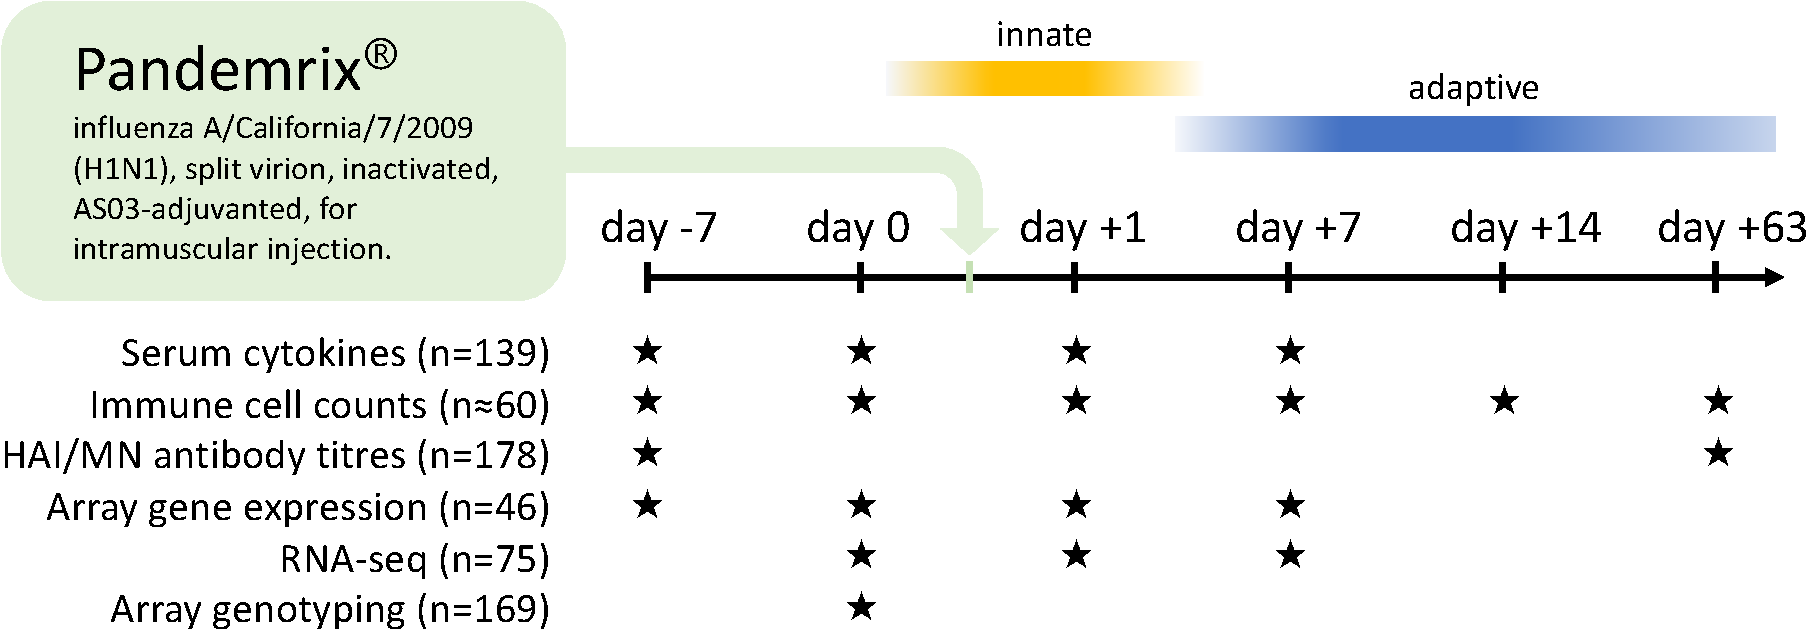
\includegraphics[width=1.0\textwidth]{mainmatter/figures/chapter_02/graphics_ashg19/hird_design-crop.pdf}
    \caption{
        \textbf{Overview of study data.}
        The total \gls{HIRD} cohort size was 178 individuals.
        % Individuals were vaccinated after day 0 sampling.
        Serum cytokines were quantified by 16-plex Luminex panel.
        Immune cell subsets were quantified by \gls{FACS}.
        Serum antibodies were quantified by both \gls{HAI} and \gls{MN} assays.
        Array and \gls{RNAseq} gene expression were quantified in the \gls{PBMC} compartment.
    }
    \label{fig:hird_design}
\end{figure}

\subsection{Computing baseline-adjusted measures of antibody response}
\label{subsec:hird_dge_TRI}

% TODO: The power of a binary hypothesis test is the probability that the test rejects the null hypothesis ( H 0 {\displaystyle H_{0}} H_{0}) when a specific alternative hypothesis ( H 1 {\displaystyle H_{1}} H_{1}) is true. The statistical power ranges from 0 to 1, and as statistical power increases, the probability of making a type II error (wrongly failing to reject the null hypothesis) decreases.
% TODO: For comparing significance tests, a meaningful measure of efficiency can be defined based on the sample size required for the test to achieve a given task power.[9]

% TODO: http://www.dokeefe.net/pub/okeefe07cmm-posthoc.pdf
% These four variables—power, significance criterion, sample size, and population effect size—are related such that when the values of three of these are fixed, the fourth is determined (Cohen, 1988, p. 14).

% TODO: do not say power when you mean efficiency or sensitivity
% https://discourse.datamethods.org/t/responder-analysis-loser-x-4/1262

% TRI alternatives e.g. adjusted maximum fold change \autocite{hipc-chisignaturesprojectteam2017MulticohortAnalysisReveals}

There were 166/178 individuals with \gls{HAI} and \gls{MN} titres available at both baseline (day -7) and post-vaccination (day 63).
\textcite{sobolev2016AdjuvantedInfluenzaH1N1Vaccination} defined Pandemrix vaccine responders as individuals with $\ge$4-fold titre increases from day -7 to day 63 in either the \gls{HAI} or \gls{MN} assays.
This is a typical threshold for \gls{HAI} and \gls{MN} seroconversion used to assess the immunogenicity of seasonal \glspl{IIV} \autocite{krammer2019HumanAntibodyResponse}, 
and has also been recommended for pandemic \glspl{IIV} \autocite{foodanddrugadministration2007GuidanceIndustryClinical}.
However, they noted there was \enquote{a complete spectrum} of baseline titres of non-responders, citing \enquote{glass ceiling} non-responders whose high baseline titres made \enquote{enhancements by \num{\ge4}-fold harder to achieve}.
This may be referring to the dynamic range of the assays.
In the full data, the range of \gls{HAI} titres is \numrange{8}{4096}, and the range of \gls{MN} titres is \numrange{10}{5120} (\cref{fig:hird_tri}a, \cref{fig:hird_tri}b).
In just the day -7 baseline titres, the range of \gls{HAI} titres is \numrange{8}{512}, and the range of \gls{MN} titres is \numrange{10}{5120}%
\footnote{
    % The means of the distributions of pre-existing titres would still be expected to be greater if this were a seasonal vaccine \autocite{tsang2014GlobalAnalysesHuman}.
    This indicates some individuals likely do have pre-existing antibodies to the pandemic strain (or cross-reactive antibodies),
    although the mean of the baseline titre distribution would still be expected to be higher if this were a seasonal vaccine.
}.
% NOTE: based on tsang2014GlobalAnalysesHuman, presumably the distribution of pre-existing titres would be higher if this was a seasonal vaccine.
It is impossible for an individual with higher than 1280 \gls{MN} at day -7 to achieve a 4-fold increase in \gls{MN} after vaccination if the maximum \gls{MN} value is \num{5120}.
This ceiling effect can been seen in \cref{fig:hird_tri}d, where for a given baseline \gls{MN} titre, there is a limit to the maximum observable fold change.

Another perspective is to consider that day 63/day -7 fold change is a change score on the log scale.
It is well-known that change scores are usually negatively correlated to baseline.
This can be due to individual-level regression to the mean%
\footnote{
    \textit{Cf.} group-level regression to the mean, which is prominent if the baseline measurement is used as a selection criteria for follow-up \autocite{barnett2004RegressionMeanWhat,senn2011FrancisGaltonRegression}.
}, 
the tendency for extreme observations to be followed by less extreme ones in the same individual \autocite{barnett2004RegressionMeanWhat},
but is also due to the mathematical relationship between change score and baseline (\enquote{mathematical coupling} \autocite{tu2007RevisitingRelationChange}).
The correlation between change score and baseline is likely to be negative 
when the variance of the post-test score is much larger than the variance of the baseline 
and the correlation between baseline and post-test score is less than one \autocite{tu2007RevisitingRelationChange,clifton2019CorrelationBaselineScore}.
% TODO: add the numerator here and explain it that way
The negative correlation of titre fold change and baseline is visible in the \gls{HIRD} data (\cref{fig:hird_tri}c, \cref{fig:hird_tri}d).

Additionally, dichotomisation of continuous variables can result in loss of information \autocite{cohen1983CostDichotomization,senn2005DichotomaniaObsessiveCompulsive,altman2006CostDichotomisingContinuous,fedorov2009ConsequencesDichotomization}.
\textcite{cohen1983CostDichotomization} presents a classic example where 
dichotomising a continuous independent variable reduces statistical power akin to throwing away a third of the samples---this being the optimal case when the cutpoint is the mean.
A discontinuous cutpoint is also biologically implausible, implying that a 4.01-fold antibody titre change would be dramatically more protective than a 3.99-fold change.

%
% \begin{outline}
% \1 Pre-process phenotypes
%     \2 Compute responder status (>= 4-fold in HAI or MN)
%     \2 Compute TRI (based on Bucasas 2009)
%         \3 “We related the change in titer between pre- and postvaccination measurements (response variable) to the prevaccination titer (explanatory variable) using a simple linear model”
%         \3 “We next determined the residuals from the above linear regressions and used them as the input values for the individual response scores.”
%         \3 “we standardised the residuals by dividing by the residual standard deviation for each component”
%             \4 Based on their axis ranges, it appears they are plotting log2(post)-log2(pre)), equivalently log2(post/pre), a.k.a. log2 fold-change; against log2(pre)
%             \4 Note that log2(post-pre) does not make sense mathematically, as post-pre may well be negative
%             \4 The negative relationship indicates lower initial titres are more amenable to high fold-change increases, which is exactly what TRI is designed to correct for
% \end{outline}
To address these concerns, I computed the \gls{TRI} as defined in \textcite{bucasas2011EarlyPatternsGene}.
For each assay, a linear regression was fit with the $\log_2{\text{day 63}/\text{day -7}}$ titre fold change as the response, and the $\log_2{\text{day -7}}$ baseline titre as the predictor.
The residuals from the two regressions were each standardised to zero mean and unit variance, then averaged with equal weight.
% NOTE: 
% This is residualised change score.
% \gls{ANCOVA} is one approach to adjusting for regression to the mean \autocite{barnett2004RegressionMeanWhat}.
The \gls{TRI} is a single variable that expresses a continuous measure of change in antibody titres averaged across both assays post-vaccination, 
compared to individuals with a similar baseline titre. 
It is no longer correlated with baseline (\cref{fig:hird_tri}e, \cref{fig:hird_tri}f),
and remains qualitatively comparable to the original binary definition (\cref{fig:hird_tri}g, \cref{fig:hird_tri}h).

\begin{figure}
    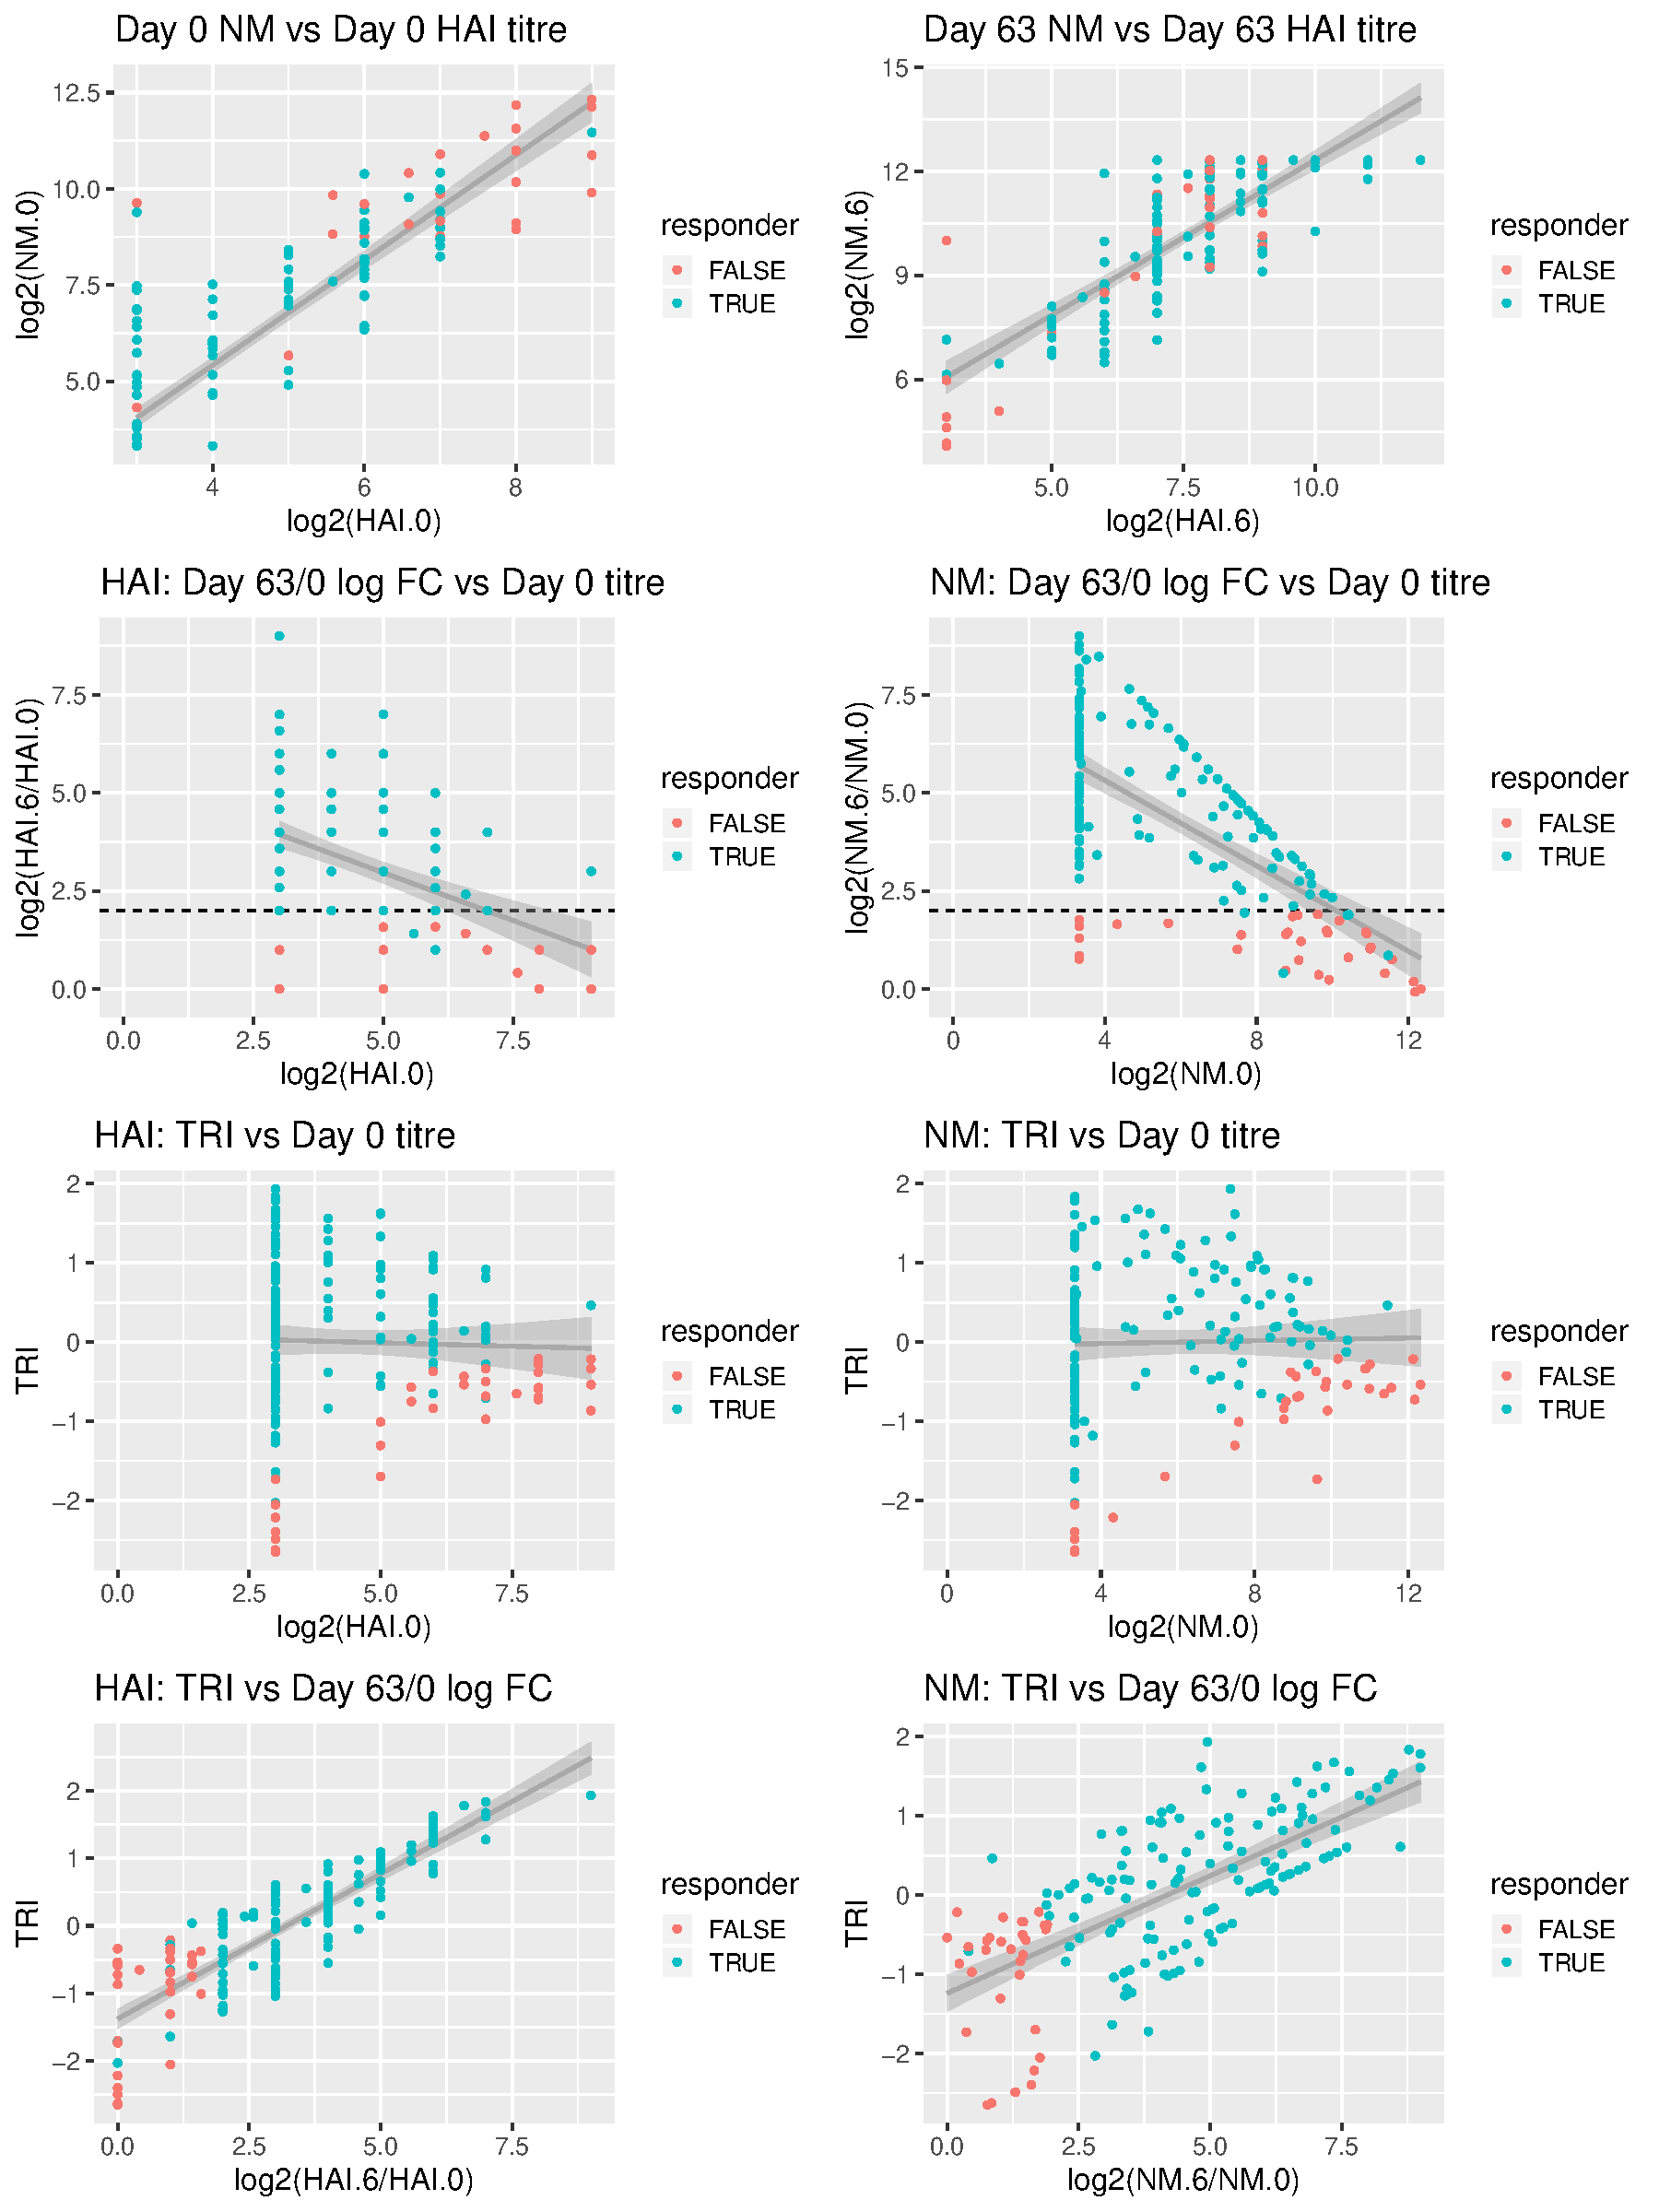
\includegraphics[width=0.95\textwidth]{mainmatter/figures/chapter_02/phenotype_data_setup.tri_comparison.pdf}
    \caption{
        \textbf{Antibody titre data and responder definitions.}
        % TODO: check n of these plots
        % Comparison of \gls{TRI} to \gls{HAI} (left column) and \gls{MN} (right column) titres and binary responder/non-responder status (colored) in 166 \gls{HIRD} individuals. 
        % Row 1: baseline titres are positively correlated to post-vaccination titres.
        Titre values are on the $\log_2$ scale.
        Individuals are colored by binary responder status: \num{\ge 4}-fold increase in either \gls{HAI} or \gls{MN} titres from baseline (day -7) to post-vaccination (day 63).
        Dashed lines show the \num{\ge 4}-fold thresholds.
        \textbf{(a, b)} \gls{HAI} and \gls{MN} titres are correlated at baseline (\textbf{a}) and post-vaccination (\textbf{b}).
        \textbf{(c, d)} Baseline titres are negatively correlated to fold change. 
        \textbf{(e, f)} \gls{TRI} is computed from the standardised residuals from \textbf{c} and \textbf{d}, adjusting for baseline titre.
        \textbf{(g, h)} \gls{TRI} remains comparable in ordering to binary response status.
    }
    \label{fig:hird_tri}
\end{figure} 

Descriptive statistics for the 114 individuals with both gene expression and antibody titre data are presented in \cref{tab:hird_table1}.
Although the proportion of responders between array (32/44) and \gls{RNAseq} (59/70) individuals is similar (\pvalue{} = \num{0.1551}, Fisher's exact test), the variance of \gls{TRI} in array individuals is higher (\pvalue{} = \num[scientific-notation=true]{0.0002098}, Levene's test), suggesting more extreme antibody response phenotypes are present (\cref{fig:hird_phenotypes_by_platform}).
% NOTE:
% Levene's test is just a t-test of the absolute values of the deviations of the data from their group means.
% [...]
% At any rate, it is a t-test, so the assumptions are based on that. Specifically, you are assuming that the absolute values of the deviations are independent, normally distributed and with equal variances between the groups. It's worth noting that these can't really be quite true.
The cause of this is unknown---there is a possibility that individuals with more extreme phenotypes were prioritised for array transcriptomics in the original \gls{HIRD} study\footnote{Personal communication with \textcite{sobolev2016AdjuvantedInfluenzaH1N1Vaccination} authors.}.

% NOTE: this table contains manual edits
% NOTE: there are no p values in this table
\begin{table}[] 
 \centering 
 \caption{\textbf{Descriptive statistics for individuals with both expression and antibody data.} Values are count and percentage for categorial variables; mean and standard deviation for continuous variables. P values are for the comparison between platforms.}\label{tab:hird_table1}
 \begin{tabular}{ l c c c }
 \toprule
  &   &  \multicolumn{ 2 }{c}{ Platform }\\ 
  & Total & Array & \gls{RNAseq} \\ 
  & n = 114 & n = 44 & n = 70 \\ 
  \midrule
 Gender &   &   &  \\ 
 \hspace{6pt}    F & 72 (63.2\%) & 27 (61.4\%) & 45 (64.3\%)\\ 
 \hspace{6pt}    M & 42 (36.8\%) & 17 (38.6\%) & 25 (35.7\%)\\ 
 Age at vaccination (years)  &   &   &  \\ 
 \hspace{6pt}   & 29.2 (11.8) & 32.9 (14.1) & 26.8 (9.4)\\ 
 Ancestry (self-reported) &   &   &  \\ 
 \hspace{6pt}    Asian & 14 (12.3\%) & 5 (11.4\%) & 9 (12.9\%)\\ 
 \hspace{6pt}    Black/African & 9 (7.9\%) & 4 (9.1\%) & 5 (7.1\%)\\ 
 \hspace{6pt}    Caucasian & 82 (71.9\%) & 33 (75\%) & 49 (70\%)\\ 
 \hspace{6pt}    Latin American & 2 (1.8\%) & 1 (2.3\%) & 1 (1.4\%)\\ 
 \hspace{6pt}    Mixed & 5 (4.4\%) & 1 (2.3\%) & 4 (5.7\%)\\ 
 \hspace{6pt}    Other - Arab & 1 (0.9\%) & 0 (0\%) & 1 (1.4\%)\\ 
 \hspace{6pt}    White Other & 1 (0.9\%) & 0 (0\%) & 1 (1.4\%)\\ 
 log2 day -7 HAI  &   &   &  \\ 
 \hspace{6pt}   & 4.4 (1.8) & 4.2 (1.6) & 4.5 (1.9)\\ 
 log2 day 63 HAI  &   &   &  \\ 
 \hspace{6pt}   & 7.6 (1.8) & 7.4 (2.2) & 7.6 (1.5)\\ 
 log2 HAI fold change  &   &   &  \\ 
 \hspace{6pt}   & 3.2 (1.9) & 3.2 (2.4) & 3.1 (1.6)\\ 
 log2 day -7 MN  &   &   &  \\ 
 \hspace{6pt}   & 6.2 (2.8) & 5.4 (2.4) & 6.6 (3.0)\\ 
 log2 day 63 MN  &   &   &  \\ 
 \hspace{6pt}   & 10.4 (2.0) & 9.5 (2.2) & 10.9 (1.6)\\ 
 log2 MN fold change  &   &   &  \\ 
 \hspace{6pt}   & 4.2 (2.3) & 4.1 (2.6) & 4.3 (2.1)\\ 
 Responder (binary definition) &   &   &  \\ 
 \hspace{6pt}    FALSE & 23 (20.2\%) & 12 (27.3\%) & 11 (15.7\%)\\ 
 \hspace{6pt}    TRUE & 91 (79.8\%) & 32 (72.7\%) & 59 (84.3\%)\\ 
 TRI &   &   &  \\ 
 \hspace{6pt}   & -0.0 (0.9) & -0.2 (1.2) & 0.1 (0.7)\\ 
 \bottomrule
 
 \end{tabular}
 \end{table}


\begin{figure}
    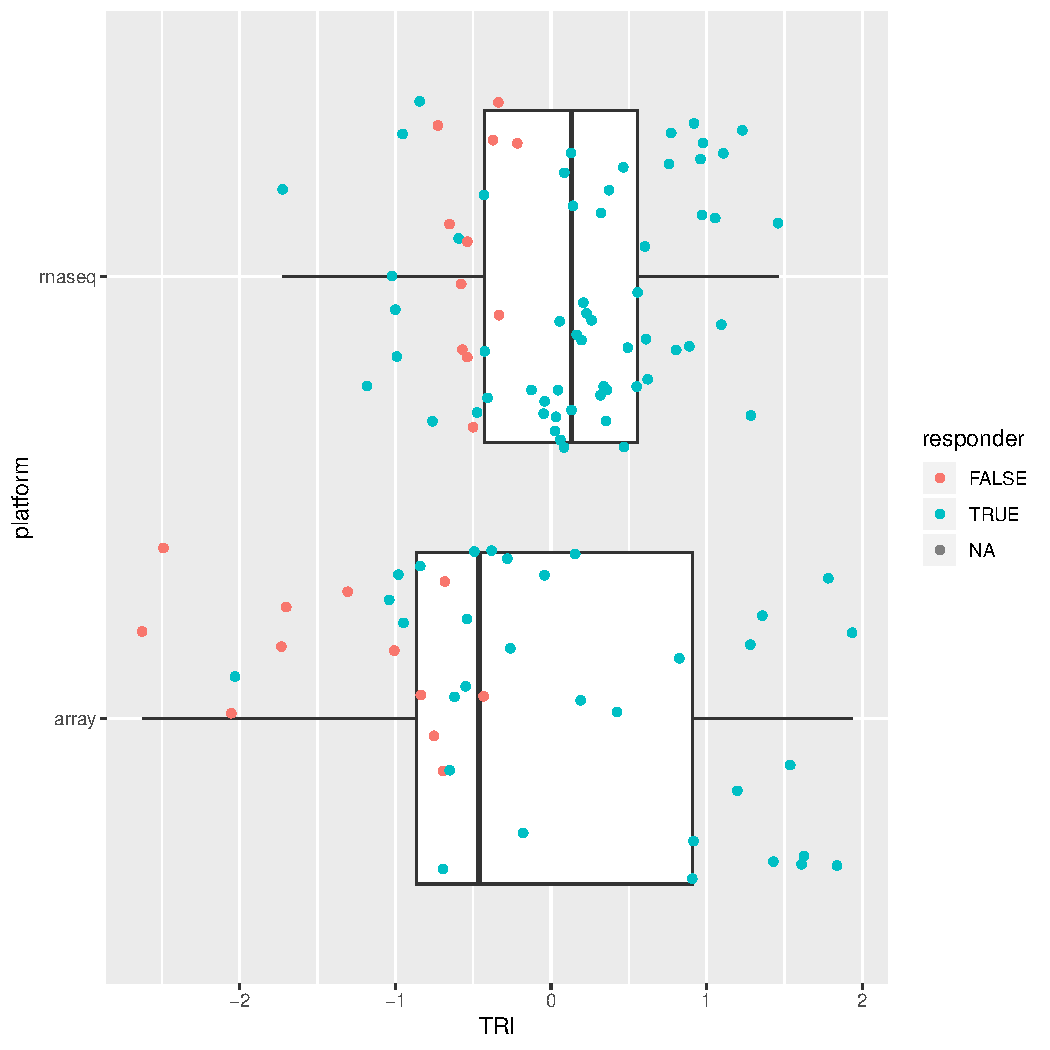
\includegraphics[width=1.0\textwidth,page=1]{mainmatter/figures/chapter_02/compare_phenotype_by_platform.pheno_boxplots.pdf}
    \caption{\textbf{Distribution of \gls{TRI}, stratified by platform.}}
    \label{fig:hird_phenotypes_by_platform}
\end{figure}

\subsection{Genotype data generation}
\label{subsec:hird_dge_genotype_data_generation}

DNA was extracted from frozen blood using the Blood and Tissue DNeasy kit (Qiagen), and genotyping was performed using on the Infinium CoreExome-24 BeadChip array (Illumina).
In total, 192 samples from 176 individuals in the \gls{HIRD} cohort---replicate samples were submitted for individuals where extracted DNA concentrations were initially low---were genotyped at \num{550601} markers

\subsection{Genotype data preprocessing}
\label{subsec:hird_dge_genotype_preproc}

Using PLINK (v1.90b3w) \autocite{chang2015SecondgenerationPLINKRising}, genotype data underwent the following quality control filters to remove poorly genotyped samples and markers:
\begin{itemize}
    \item maximum marker missingness across samples \SI{< 5}{\percent};
    \item maximum sample missingness across markers \SI{< 1}{\percent} (\cref{fig:hird_genotype_sample_hetRate_missingness});
    \item sample heterozygosity rate within 3 standard deviations of the mean of all samples (threshold selected visually to exclude outliers, \cref{fig:hird_genotype_sample_hetRate_missingness});
    \item sample sex mismatches based on X chromosome marker heterozygosity (\texttt{-{}-check-sex} option);
    % NOTE: \autocite{mccarthy2008GenomewideAssociationStudies}
    % Once armed with a set of called genotypes, the final phase of quality control beckons. Experience has shown that most SNPs showing extreme departures from Hardy–Weinberg equilibrium (HWE) in controls can be safely discarded1, although lesser (but nevertheless quite marked) departures are to be expected under the null hypothesis, given the number of tests performed. 
    % Appropriate thresholds for any given study will depend on the sample size and overall data quality, and might best be defined by using the observed distribution of HWE statistics (the WTCCC used this approach to set a threshold at an exact p < 5.7 × 10−7 in controls)1. In any event, HWE is an imprecise tool for quality control purposes. Tests of departure from HWE are underpowered for the detection of genotyping error75,76, whereas overenthusiastic use of HWE as a quality criterion can prove to be counterproductive given that modest disequilibrium (in cases particularly) can be a signature of true association.
    %
    % NOTE: \autocite{anderson2010DataQualityControl}
    % Most GWA studies choose to exclude markers that show extensive deviation from Hardy-Weinberg equilibrium (HWE) because this can be indicative of a genotyping or genotype calling error. However, deviations from Hardy-Weinberg equilibrium may also indicate selection, so a case sample can show deviations from HWE at loci associated with disease, and it would obviously be counter-productive to remove these loci from further investigation 18. Therefore, only control samples should be used when testing for deviations for HWE.
    % The significance threshold for declaring SNPs to be in Hardy-Weinberg equilibrium has varied greatly between studies (p-value thresholds between 0.001 and 5.7 × 10−7 have been reported in the literature3,19).
    \item and marker deviation from \gls{HWE}, an indication of genotyping or genotype calling errors \autocite{mccarthy2008GenomewideAssociationStudies,anderson2010DataQualityControl,marees2018TutorialConductingGenomewide} (\texttt{-{}-hwe} option, \pvalue{} \num[scientific-notation=true]{< 0.00001})%
        \footnote{
            A wide range of thresholds for the \gls{HWE} marker filter in controls between \num{1.0e-3} and \num{5.7e-7} are reported in the literature \autocite{anderson2010DataQualityControl}.
            The \gls{HWE} threshold used here is from \textcite{delange2017GenomewideAssociationStudy};
            since the \gls{HIRD} cohort is two orders of magnitude smaller in size, this represents a relaxed threshold, so additional vigilance for genotyping errors downstream is required.
            In principle, it may be possible to select an appropriate threshold from the empirical distribution of \gls{HWE} \pvalues{} \autocite{mccarthy2008GenomewideAssociationStudies}.
        }.
\end{itemize}

\begin{figure}
    \includegraphics[width=1.0\textwidth,page=2]{mainmatter/figures/chapter_02/coreex_eQTLflu_20171204.gencall.smajor.impute_sex.qc2.pdf}
    \caption{
        \textbf{Sample filters for marker missingness and marker heterozygosity rate.}
        Thresholds for missingness (\SI{1}{\percent}) and heterozygosity rate (mean $\pm$ 3 standard deviations) are shown by dashed lines.
    }
    \label{fig:hird_genotype_sample_hetRate_missingness}
\end{figure}

To exclude closely-related individuals and deduplicate samples from the same individual, 
pairwise kinship coefficients were computed using KING (v1.4) \autocite{manichaikul2010RobustRelationshipInference}.
% NOTE:
% http://people.virginia.edu/~wc9c/KING/manual.html#WITHIN
% Genome-wide SNPs are required in KING. Please do not prune or filter any "good" SNPs that pass QC prior to any KING inference, unless the number of variants is too many to fit the computer memory, e.g., > 100,000,000 as in a WGS study, in which case rare variants can be filtered out. LD pruning is not recommended in KING.
As rare variation is not generally required to determine relatedness, 
markers were filtered to \gls{MAF} \num{> 0.05} for computational efficiency.
For each pair of samples with pairwise kinship coefficient \num{> 0.177} (first-degree relatives or closer), the sample with lower marker missingness was selected.
After all filters, 169/176 samples and \num{549414/550601} markers remained.

\subsection{Computing genotype \glsfmtlongpl{PC} as covariates for ancestry}
\label{subsec:hird_dge_genotype_pc}

As shown in \cref{tab:hird_table1}, the \gls{HIRD} cohort is multi-ethnic.
Large-scale population structure explains variation in gene expression \autocite{stegle2012UsingProbabilisticEstimation,brown2018ExpressionReflectsPopulation}, 
so including genotype \glspl{PC} that reflect that structure as covariates can increase statistical efficiency for detecting associations with expression.
I used HapMap 3 samples \autocite{theinternationalhapmap3consortium2010IntegratingCommonRare} as a reference population of unrelated individuals where the major axes of variation in genotypes are ancestry.
Genotypes were first \gls{LD}-pruned (PLINK \texttt{-{}-indep-pairwise 50 5 0.2} i.e. in a sliding window of \SI{50}{\kilo\bp}, with a step size of 5 variants, remove variants at each step until no pair of variants has \gls{LD} \num[round-precision=1]{>0.2}), 
to avoid regions with many redundant markers being overrepresented in the resulting \glspl{PC} \autocite{price2006PrincipalComponentsAnalysis,abdellaoui2013PopulationStructureMigration}.
% /lustre/scratch119/realdata/mdt2/teams/barrett/coreex_gaibdc/refs/high-LD-regions.txt
% 1 48000000 52000000 1
% 2 86000000 100500000 2
% 2 183000000 190000000 3
% 3 47500000 50000000 4
% 3 83500000 87000000 5
% 5 44500000 50500000 6
% 5 129000000 132000000 7
% 6 25500000 33500000 8
% 6 57000000 64000000 9
% 6 140000000 142500000 10
% 7 55000000 66000000 11
% 8 8000000 12000000 12
% 8 43000000 50000000 13
% 8 112000000 115000000 14
% 10 37000000 43000000 15
% 11 87500000 90500000 16
% 12 33000000 40000000 17
% 20 32000000 34500000 18
Eighteen genomic regions with especially strong and/or long-range \gls{LD} that contain many highly correlated markers were excluded, otherwise some \glspl{PC} may reflect those just regions rather than genome-wide ancestry \autocite{price2006PrincipalComponentsAnalysis,prive2020EfficientToolkitImplementing}.
\Gls{PCA} was performed using smartpca (v8000) \autocite{price2006PrincipalComponentsAnalysis},
then \gls{HIRD} sample \glspl{PC} were computed by projection onto the HapMap 3 \gls{PCA} eigenvectors.
%
% http://www.biostatgen.org/wp-content/uploads/2018/09/bby081.pdf 
% If we assume that the correlation structure itselfdiffers between cases and controls, then it makes sense to do thePCA on controls and then project its results on cases as discussedin [71]. However, if we assume that the structure itself may bethe same, but just the factor values are different, then we coulduse the entire group for the PCA to have a larger sample sizeand obtain more stable results.
A projection was used instead of in-sample \gls{PCA}, as cryptic relatedness in \gls{HIRD} may be reflected in the resulting \glspl{PC} instead of ancestry \autocite{price2010NewApproachesPopulation}.
For non-genotyped individuals with expression data, 
\gls{PC} values were imputed as the mean value for all genotyped individuals with the same self-reported ancestry.
The top \glspl{PC} indeed separate \gls{HIRD} samples by ancestry (\cref{fig:hird_genotype_pca_withHapmap}).
% Thus, we expect that the theoretical covariance matrix (approximated by the sample covariance) will have K − 1 “large” eigenvalues, with the remainder small and reflecting the sampling variance.
Significant \glspl{PC} with large eigenvalues unlikely to be due to sampling noise were selected by Tracy-Widom test \autocite{patterson2006PopulationStructureEigenanalysis}.
The fourth \gls{PC} had an eigenvalue of \num{1.005305} (\pvalue{} = \num{0.0238744}), 
so the top four \glspl{PC} were retained as continuous covariates for ancestry downstream.

\begin{figure}
    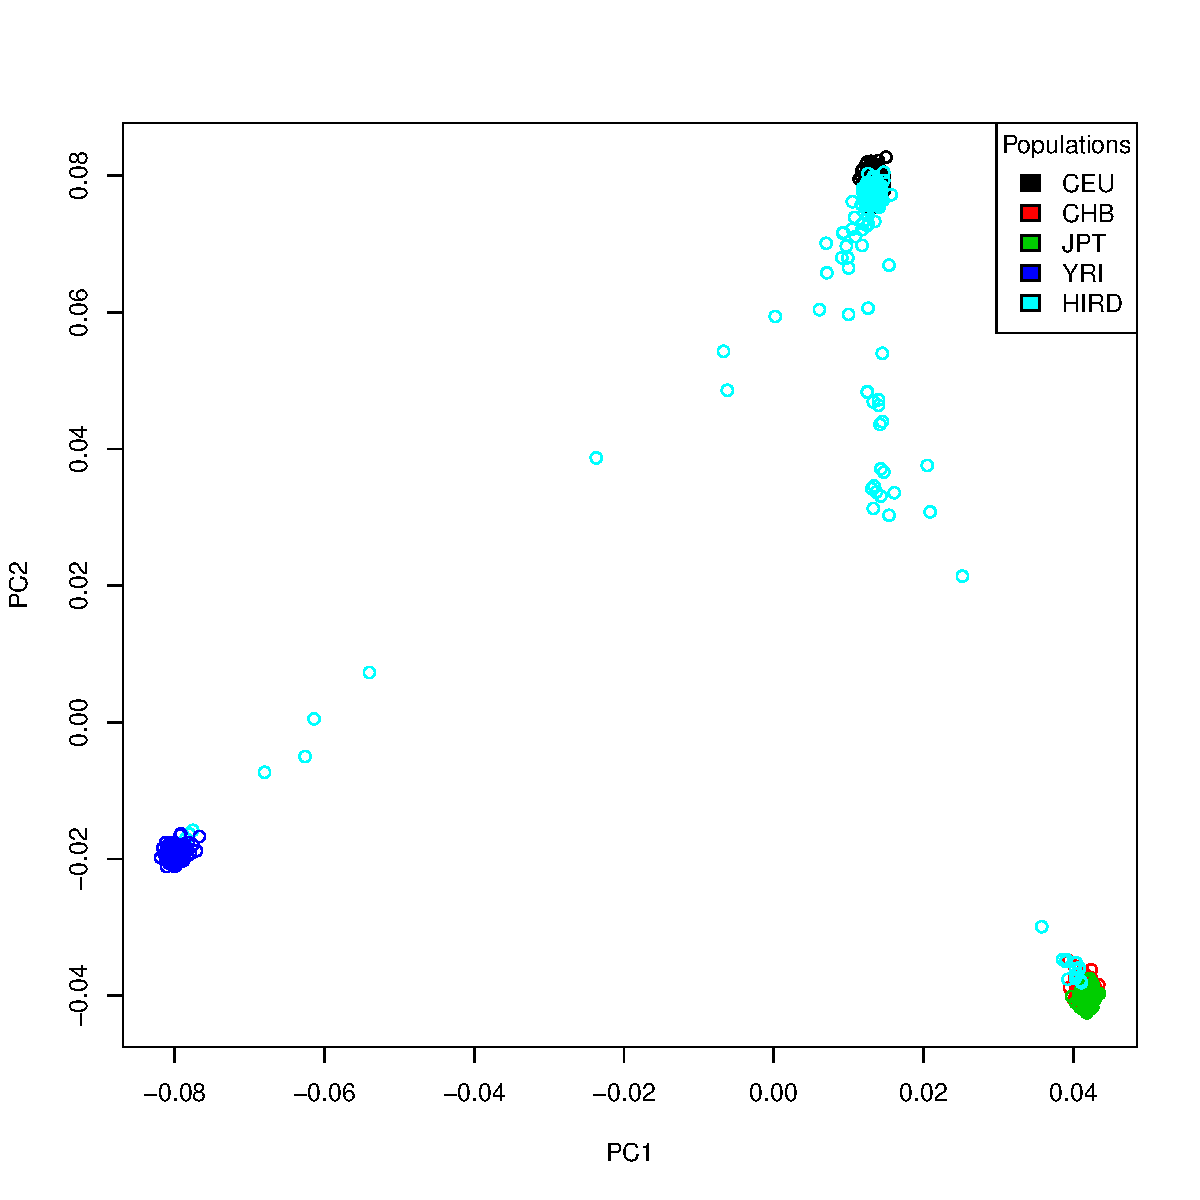
\includegraphics[width=1.0\textwidth]{mainmatter/figures/chapter_02/coreex_eQTLflu_20171204.gencall.smajor.impute_sex.qc3.pruned.hapmap_merged.flipped.pca.evec.pdf}
    \caption{
        \textbf{\gls{HIRD} samples (cyan) projected onto \gls{PC}1 and \gls{PC}2 axes defined by \gls{PCA} of HapMap 3 samples.}
        The first two \glspl{PC} separate individuals of European (CEU, upper-right) from Asian (CHB and JPT, lower-right) and African (YRI, lower-left).
    }
    \label{fig:hird_genotype_pca_withHapmap}
\end{figure}

\subsection{\glsfmtshort{RNAseq} data generation}

Total RNA was extracted from \glspl{PBMC} using the Qiagen RNeasy Mini kit, with on-column DNase treatment.
RNA integrity was checked on the Agilent Bioanalyzer and mRNA libraries were prepared with the KAPA Stranded mRNA-Seq Kit (KK8421), which uses poly(A) selection.
% 7 lanes x 3 plates
To avoid confounding of timepoint and technical effects from library preparation and sequencing,
samples were pooled by library preparation plate (three pools) ensuring libraries from all timepoints of an individual were in the same pool, 
then sequenced across multiple lanes as technical replicates (HiSeq 4000, \SI{75}{\bp} paired-end).
% TODO:
% examples of failures of RNAseq design https://f1000research.com/articles/4-121/v1
% TODO: this is deliberate confounding: schielzeth2013NestedDesignModel
% although patient nested in plate. patient x plate interaction is confounded with main effect of patient
% we are not interested in this
% TODO: this is correct:
% Checking that I understand the sources of technical variability, is it that
% all the samples in each pool will go through library prep together (e.g. same
% plate, reagent batch, roughly same time), and then be barcoded and sequenced
% on the same (lane of the) Novaseq flow cell?
%
% TODO:
% Design and validation issues in RNA-seq experiments

% To get to cram files:
% From .cram headers:
% 1.	The NextSeq, HiSeq, and NovaSeq Sequencing Systems generate raw data files in binary base call (BCL) format.
% 1.1.	HiSeq Sequencing Control Software (SCS), version HD 3.4.0.38, used for basecalling
% 2.	biobambam2/bamadapterfind: bamdapterfind scans a BAM file for contaminations by sequencing adapters.
% 3.	bambi decode: decode a multiplexed bam file
% 4.	bwa sampe (alignment using BWA-backtrack): alignment to phiX, which is then merged with the original bam
% 5.	pb_calibration/spatial_filter: Identify regions with spatially correlated errors e.g. bubbles, (from aligned BAM files where the read name can be parsed for spatial location) and allow filtering out or marking of the BAM fail bit for reads in those regions.
% 6.	Alignment with tophat 2.0.14
% 6.1.	 --keep-fasta-order --no-sort-bam --output-dir tophat_out_24165_1#10 --mate-inner-dist 100 --num-threads=8 --library-type=fr-firststrand --no-coverage-search --microexon-search --transcriptome-index=/lustre/scratch117/core/sciops_repository/transcriptomes/Homo_sapiens/ensembl_83_transcriptome/GRCh38_15_plus_hs38d1/tophat2/GRCh38_15_plus_hs38d1.known/lustre/scratch117/core/sciops_repository/references/Homo_sapiens/GRCh38_15_plus_hs38d1/all/bowtie2/Homo_sapiens.GRCh38_15_plus_hs38d1.fa
% 7.	Some sort of duplicate marking and filtering (?) using some combination of:
% 7.1.	biobambam/bamsormadup: parallel sorting and duplicate marking
% 7.2.	uk.ac.sanger.npg.picard.AlignmentFilter
% 7.3.	biobambam/bamstreamingmarkduplicates
% 8.	Write .cram files using scramble (cram is a reference-based compression)
% 8.1.	/lustre/scratch117/core/sciops_repository/references/Homo_sapiens/GRCh38_15_plus_hs38d1/all/fasta/Homo_sapiens.GRCh38_15_plus_hs38d1.fa
% 9.	NOTE: Note lots of intermediate biobambam 2.0.76 and scramble processing steps, not all are listed.

% TODO: Can add other fastqc plots e.g. kmers, overrepresented seqs, seq length
% Genomic origin of reads and gene end biases were assessed using Qualimap, after aligning the reads to the human GRCh38_15_plus_hs38d10 reference transciptome using tophat2.
\gls{RNAseq} quality metrics were assessed using FastQC\footnote{\url{https://www.bioinformatics.babraham.ac.uk/projects/fastqc/}} and Qualimap \autocite{okonechnikov2015QualimapAdvancedMultisample}, then visualised with MultiQC \autocite{ewels2016MultiQCSummarizeAnalysis}.
% See log 2017-11-20 for fastqc discussion
Sequence quality was high, as measured by mean per-base Phred scores across sample reads (\cref{fig:hird_fastqc_seqQual}).
% Sequence duplication levels were acceptable for \gls{RNAseq} (\cref{fig:hird_fastqc_seqDupe}).
The unimodal GC-content distribution suggested negligible levels of non-human contamination (\cref{fig:fastqc_gc}).

\begin{figure}
	\centering
	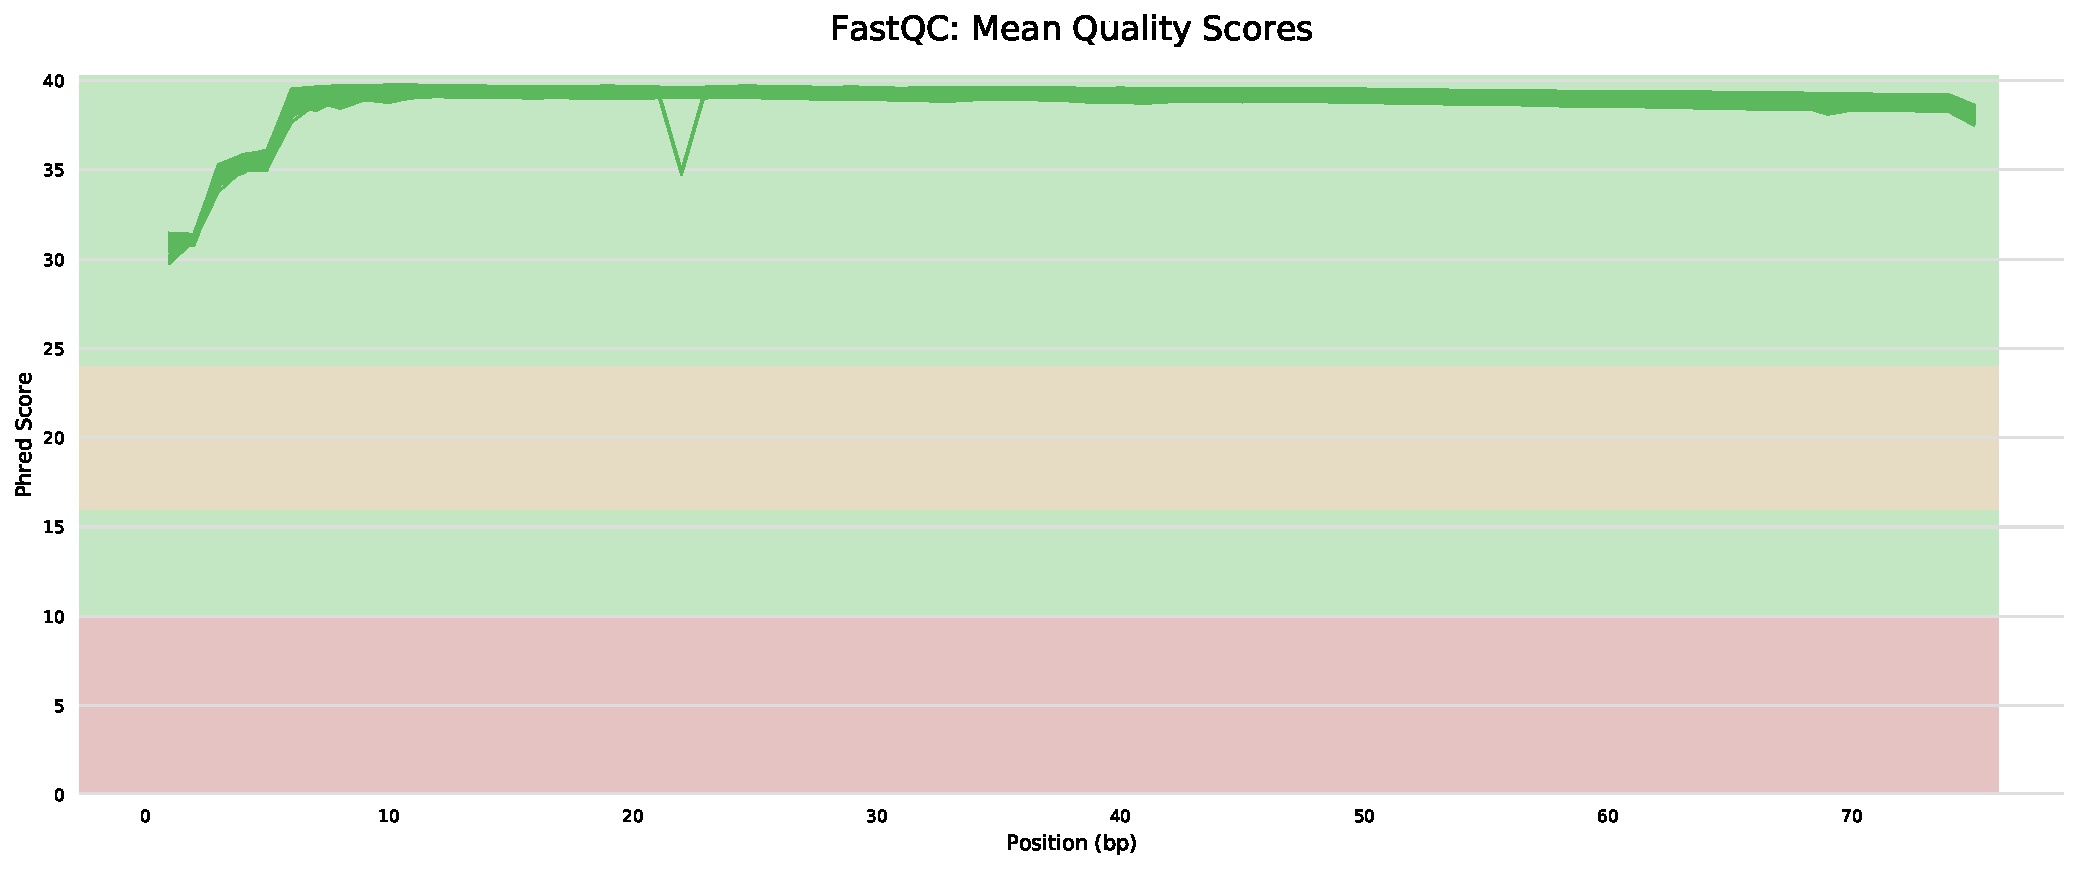
\includegraphics[width=\textwidth]{mainmatter/figures/chapter_02/graphics_firstYearReport/fastqc/mqc_fastqc_per_base_sequence_quality_plot_1.pdf}
    \caption{
        \textbf{FastQC per-base sequence quality (Phred scores) versus read position for \gls{RNAseq} samples.}
        Visualised with MultiQC \autocite{ewels2016MultiQCSummarizeAnalysis}.
    }
	\label{fig:hird_fastqc_seqQual}
\end{figure}

% \begin{figure}
%     \centering
%     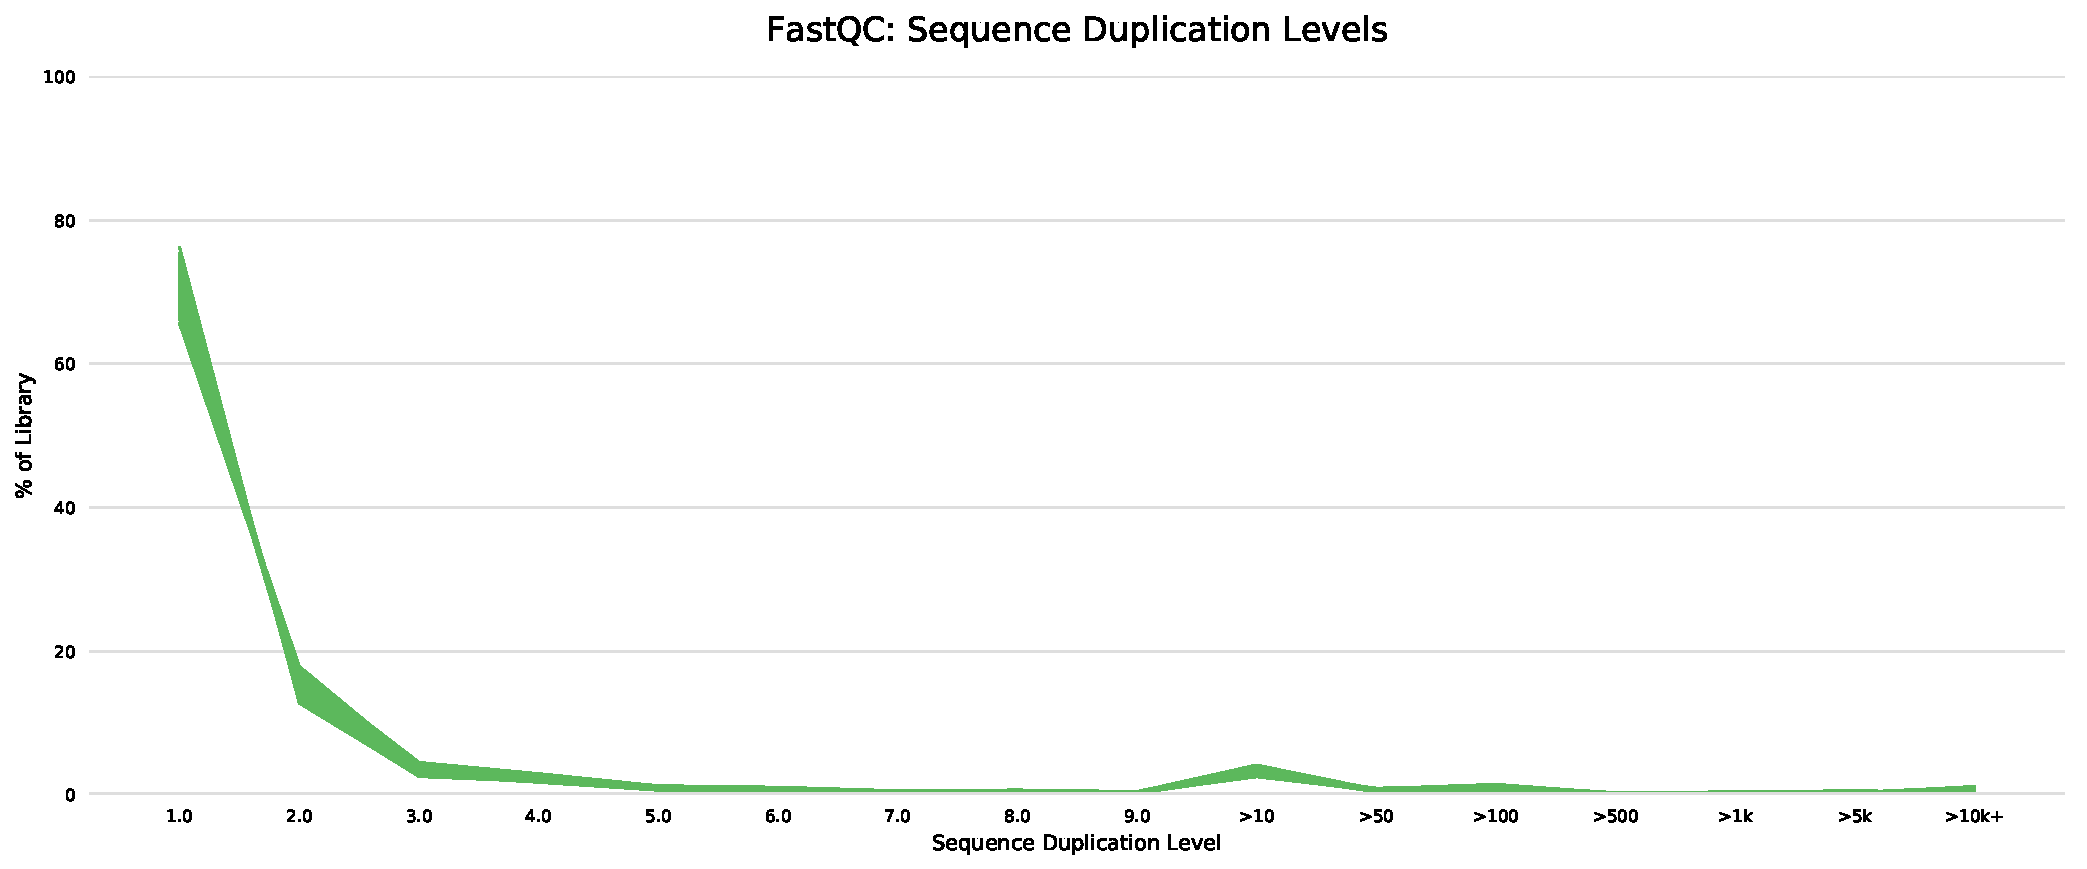
\includegraphics[width=\textwidth]{mainmatter/figures/chapter_02/graphics_firstYearReport/fastqc/mqc_fastqc_sequence_duplication_levels_plot_1.pdf}
%     \caption{FastQC sequence duplication levels for \gls{HIRD} \gls{RNAseq} samples.}
%     \label{fig:hird_fastqc_seqDupe}
% \end{figure}

\begin{figure}
	\centering
	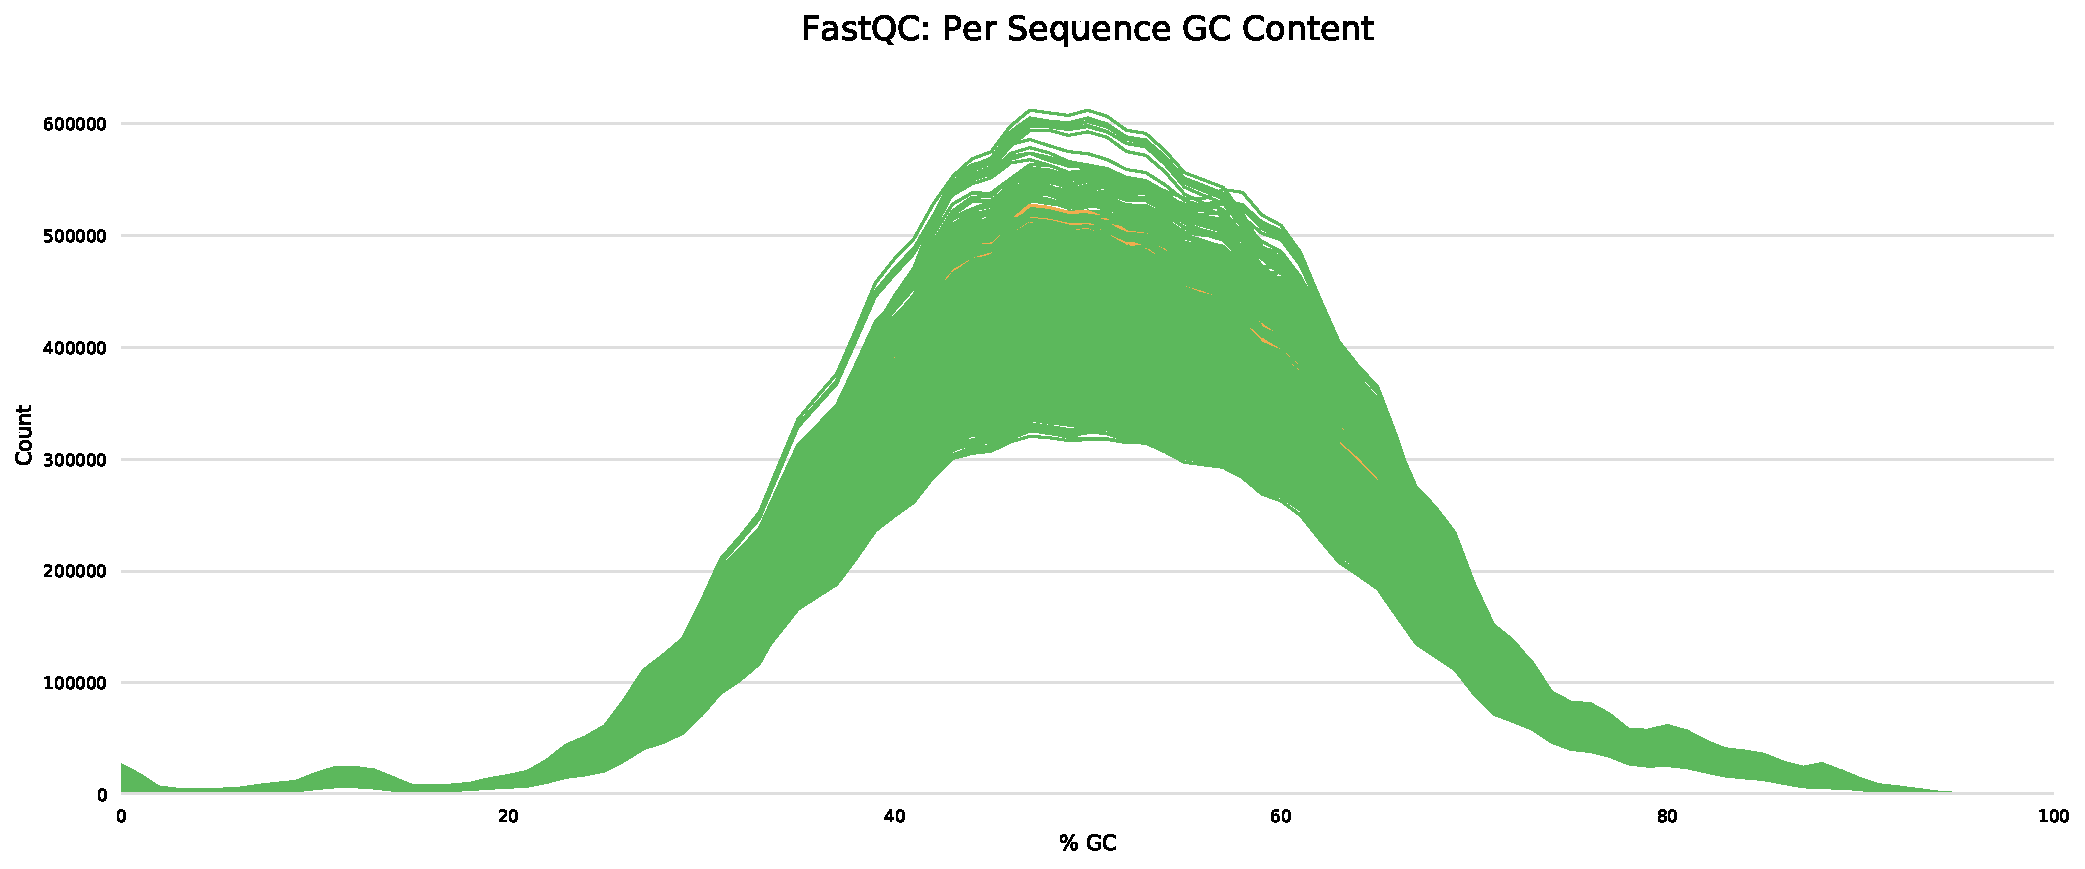
\includegraphics[width=\textwidth]{mainmatter/figures/chapter_02/graphics_firstYearReport/fastqc/mqc_fastqc_per_sequence_gc_content_plot_Counts.pdf}
    \caption{
        \textbf{FastQC per-read GC distributions for \gls{RNAseq} samples.}
        Visualised with MultiQC \autocite{ewels2016MultiQCSummarizeAnalysis}.
}
	\label{fig:fastqc_gc}
\end{figure}

\subsection{\glsfmtshort{RNAseq} quantification and preprocessing}
\label{subsec:hird_dge_rnaseq_quantAndFilter}

% 1.	Quantification (Salmon --libType ISR, which is equiv to TopHat -fr-firststrand with paired end data)
% 1.1.	Used index /lustre/scratch117/core/sciops_repository/transcriptomes/Homo_sapiens/ensembl_83_transcriptome/GRCh38_15_plus_hs38
% 1.1.1.	This is GRCh38.p5, Dec 2017, v83; with additional hs38d1: Decoy version 1 for GRCh38
% 1.1.2.	Contains ENST transcript ids
% 1.2.	Output quantifies transcripts in terms of: TPM — This is salmon’s estimate of the relative abundance of this transcript in units of Transcripts Per Million (TPM). TPM is the recommended relative abundance measure to use for downstream analysis.
% 1.2.1.	https://haroldpimentel.wordpress.com/2014/05/08/what-the-fpkm-a-review-rna-seq-expression-units/ TPM = (count/effectiveLength) / sumOverAllTranscripts(count/effectiveLength)
% 1.3.	Note Salmon also takes into account: EffectiveLength — This is the computed effective length of the target transcript. It takes into account all factors being modeled that will effect the probability of sampling fragments from this transcript, including the fragment length distribution and sequence-specific and gc-fragment bias (if they are being modeled).
% 2.	Gene-level regeneration of counts (tximport)
% 2.1.	“generate estimated counts using abundance estimates scaled up to library size (scaledTPM)”
% 2.1.1.	Note, we do not scale for gene length, that would be lengthScaledTPM. Hence the generated counts remain length-corrected.
% 2.2.	Summarizes using a mapping of ENST to ENSG, generated from /lustre/scratch117/core/sciops_repository/transcriptomes/Homo_sapiens/ensembl_83_transcriptome/GRCh38_15_plus_hs38d1/gtf/ensembl_83_transcriptome-GRCh38_15_plus_hs38d1.gtf
% 2.3.	Counts from all lanes of a sample are summed
% 3.	GC bias, length bias, mappability
% 3.1.	Length bias only affects RNAseq: somewhat alleviated by Salmon using effective length
% 3.2.	GC bias affects both technologies: somewhat alleviated by Salmon using effective length (see the salmon paper)
% NOTE:
% 3.3.	Mappability has not been considered
%
% NOTE: Salmon is not pseudo-alignment: "Unlike pseudoalignment, Salmon’s lightweight mapping procedure tracks, by default, the position and orientation of all mapped fragments."
% TODO: Add pros and cons vs regular alignment
% https://www.ncbi.nlm.nih.gov/pmc/articles/PMC6042521/ Limitations of alignment-free tools in total RNA-seq quantification
Reads were quantified against the Ensembl reference transcriptome (GRCh38.p15) using Salmon \autocite{patro2017SalmonProvidesFast} in quasi-mapping-based mode, 
which internally corrects for transcript length and GC composition by computing an effective length for each transcript.
% NOTE: Two biases are library composition and feature length in RNAseq
% scaledTPM or lengthScaledTPM is still adjusted for feature length
%
% We could alternatively generate counts from abundances, using the argument countsFromAbundance, scaled to library size, "scaledTPM", or additionally scaled using the average transcript length, averaged over samples and to library size, "lengthScaledTPM". Using either of these approaches, the counts are not correlated with length, and so the length matrix should not be provided as an offset for downstream analysis packages.
Relative transcript abundances were summarised to Ensembl (release 90) gene-level count estimates using \software{tximport} (\texttt{scaledTPM} method, which scales Salmon \gls{TPM} values up to the library size \autocite{soneson2016DifferentialAnalysesRNAseq,love2018SwimmingDownstreamStatistical}) to improve statistical robustness and interpretability \autocite{soneson2016DifferentialAnalysesRNAseq}.
% NOTE: in future, just combine technical replicates at the read level
To combine technical replicates, as the sum of Poisson distributions remains Poisson-distributed, counts for technical replicates were summed for each sample.
The mean number of mapped read pairs per sample after summing was 27.09 million read pairs (range \numrange{20.24}{39.14} million), representing a mean mapping rate of \SI{80.73}{\percent} (range \SIrange{75.57}{90.10}{\percent}).
These meet sequencing depth recommendations for \gls{DGE} experiments
(e.g. diminishing returns after 10 million single-end reads \autocite{liu2014RNAseqDifferentialExpression}) 
and mapping rate expectations 
(e.g. \SIrange{70}{90}{\percent} \autocite{conesa2016SurveyBestPractices}).
% Also see:
%
% https://genomebiology.biomedcentral.com/articles/10.1186/s13059-016-0881-8
% "While some authors will argue that as few as five million mapped reads are sufficient to quantify accurately medium to highly expressed genes in most eukaryotic transcriptomes, others will sequence up to 100 million reads to quantify precisely genes and transcripts that have low expression levels [7]."
%
% https://genome.ucsc.edu/ENCODE/protocols/dataStandards/ENCODE_RNAseq_Standards_V1.0.pdf
% 2. Sequencing depth.
% The amount of sequencing needed for a given sample is determined by the goals of the experiment and the nature of the RNA sample.
% Experiments whose purpose is to evaluate the similarity between the transcriptional profiles of two polyA+ samples may require only modest depths of sequencing (e.g. 30M pair-end reads of length > 30NT, of which 20-25M are 3mappable to the genome or known transcriptome, Experiments whose purpose is discovery of novel transcribed elements and strong quantification of known transcript isoforms requires more extensive sequencing.
% The ability to detect reliably low copy number transcripts/isoforms depends upon the depth of sequencing and on a sufficiently complex library.
% For experiments from a typical mammalian tissue or in which sensitivity of detection is important, a minimum depth of 100-200 M 2 x 76 bp or longer reads is currently recommended.

% 5.	Pre-process RNA-seq expression data
% 5.1.	Pull in tximport counts
% 5.1.1.	60675 loci, 223 samples
% 5.2.	Add gene annotation based on EnsDb.Hsapiens.v86
% 5.3.	Low-count filtering (>0.5 CPM in 10% of 223 samples i.e. 22 samples)
% Max zero prop: need to be stringent as limma doesn't account for neg bin
% 5.4.	Remove globin genes and short 
% 5.4.1.	Human globins: https://en.wikipedia.org/wiki/Globin#Examples
% 5.4.2.	Short non-coding GENEBIOTYPES: https://www.gencodegenes.org/pages/biotypes.html
% 5.5.	NOTE: we have not yet removed GENEBIOTYPE=NA. These may be retired ids.
Genes with short \gls{ncRNA} biotypes\footnote{miRNA, miRNA\_pseudogene, miscRNA, miscRNA pseudogene, Mt rRNA, Mt tRNA, rRNA, scRNA, snlRNA, snoRNA, snRNA, tRNA, tRNA\_pseudogene. List from \url{https://www.ensembl.org/Help/Faq?id=468}} were filtered out.
% They are not well captured by regular RNAseq protocols
These are generally not polyadenylated, depleted by size selection during library preparation, and shorter than the \SI{75}{\bp} read length, so expression estimates for these genes can reflect misassignment of counts from overlapping protein-coding or long \gls{ncRNA} genes \autocite{zhao2018EvaluationTwoMain}.
% Reticulocytes are immature red blood cells (RBCs).
%
% Globins
% ENSG00000161544,CYGB
% ENSG00000206172,HBA1
% ENSG00000188536,HBA2
% ENSG00000244734,HBB
% ENSG00000223609,HBD
% ENSG00000213931,HBE1
% ENSG00000213934,HBG1
% ENSG00000196565,HBG2
% ENSG00000206177,HBM
% ENSG00000086506,HBQ1
% ENSG00000130656,HBZ
% ENSG00000198125,MB
Globin genes, which are highly expressed in \glspl{RBC} and reticulocytes---cell types expected to be depleted in \gls{PBMC} \autocite{min2010VariabilityGeneExpression}---were also filtered out.
Given the proportion of removed counts at this stage was low for most samples (\cref{fig:hird_shortncRNA_and_globins}), 
poly(A) selection and \gls{PBMC} isolation were deemed to have been efficient.

\begin{figure}
    \centering
    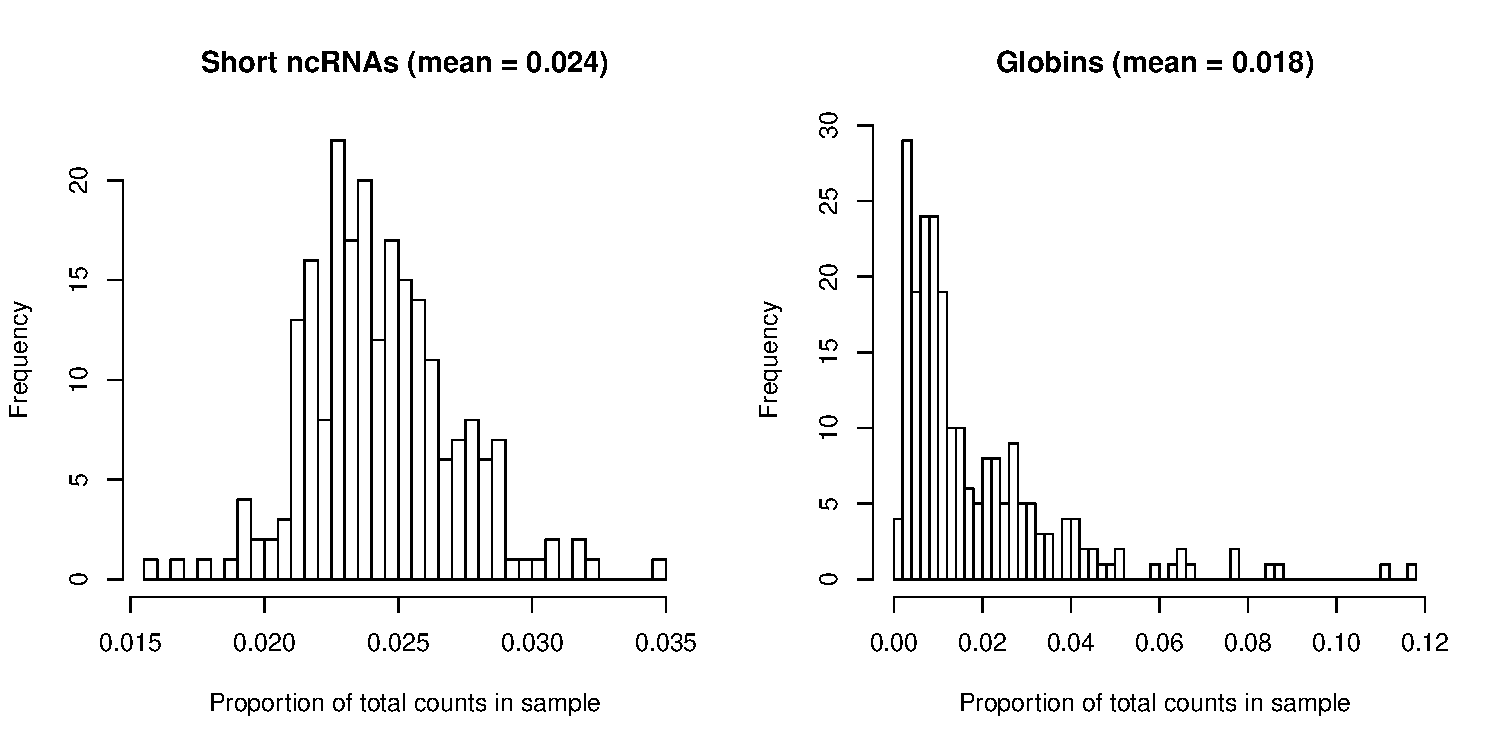
\includegraphics[width=1.0\textwidth, page=1]{mainmatter/figures/chapter_02/rnaseq_data_setup.per_sample.short_ncRNA_globin_levels_hist.pdf}
    \caption{\textbf{Distributions of removed short \gls{ncRNA} and globin counts as a proportion of total counts in \gls{RNAseq} samples.}}
    \label{fig:hird_shortncRNA_and_globins}
\end{figure}

Many of the genes in the reference transcriptome were not detectably expressed in \gls{PBMC} (\cref{fig:hird_rnaseq_filtering_zeroProp}), and many genes were expressed at counts too low for statistical analysis of \gls{DGE}.
% NOTE: no TMM was done before this CPM calculation
Genes were filtered to require a minimum of 0.5 \gls{CPM} in at least \SI{20}{\percent} of samples.
% NOTE: smallest library was 18.7M read pairs
The 0.5 \gls{CPM} threshold was chosen to correspond to approximately 10 counts in the smallest library, where \numrange{10}{15} counts is a rule of thumb for considering a gene to be robustly expressed \autocite{chen2016ReadsGenesPathways,law2018RNAseqAnalysisEasy}.
Genes were further filtered to require detection (non-zero expression) in at least \SI{95}{\percent} of samples to lessen the impact of low-expression outliers.
The change in the distributions of gene expression among samples before and after filtering shows a substantial number of low expression genes are removed (\cref{fig:hird_rnaseq_cpm_filtering}).

\begin{figure}
    \centering
    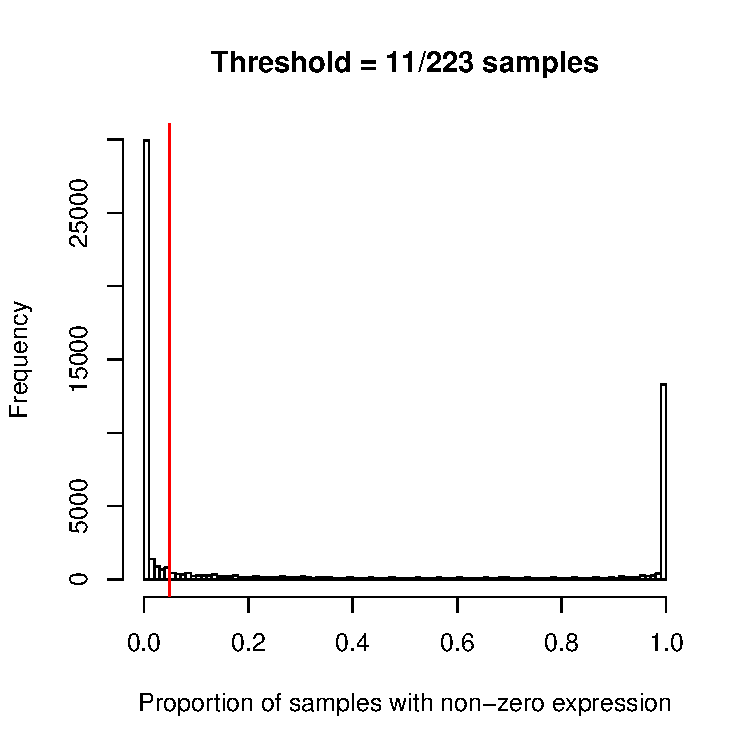
\includegraphics[width=0.6\textwidth, page=1]{mainmatter/figures/chapter_02/rnaseq_data_setup.gene_zero_prop.pdf}
    \caption{
        \textbf{Distribution of the proportion of samples in which genes were detected (non-zero expression).}
        Many genes are not detected in any samples (left-hand side). 
        Vertical line shows \SI{5}{\percent} threshold below which genes were discarded.
    }
    \label{fig:hird_rnaseq_filtering_zeroProp}
\end{figure}

\begin{figure}
    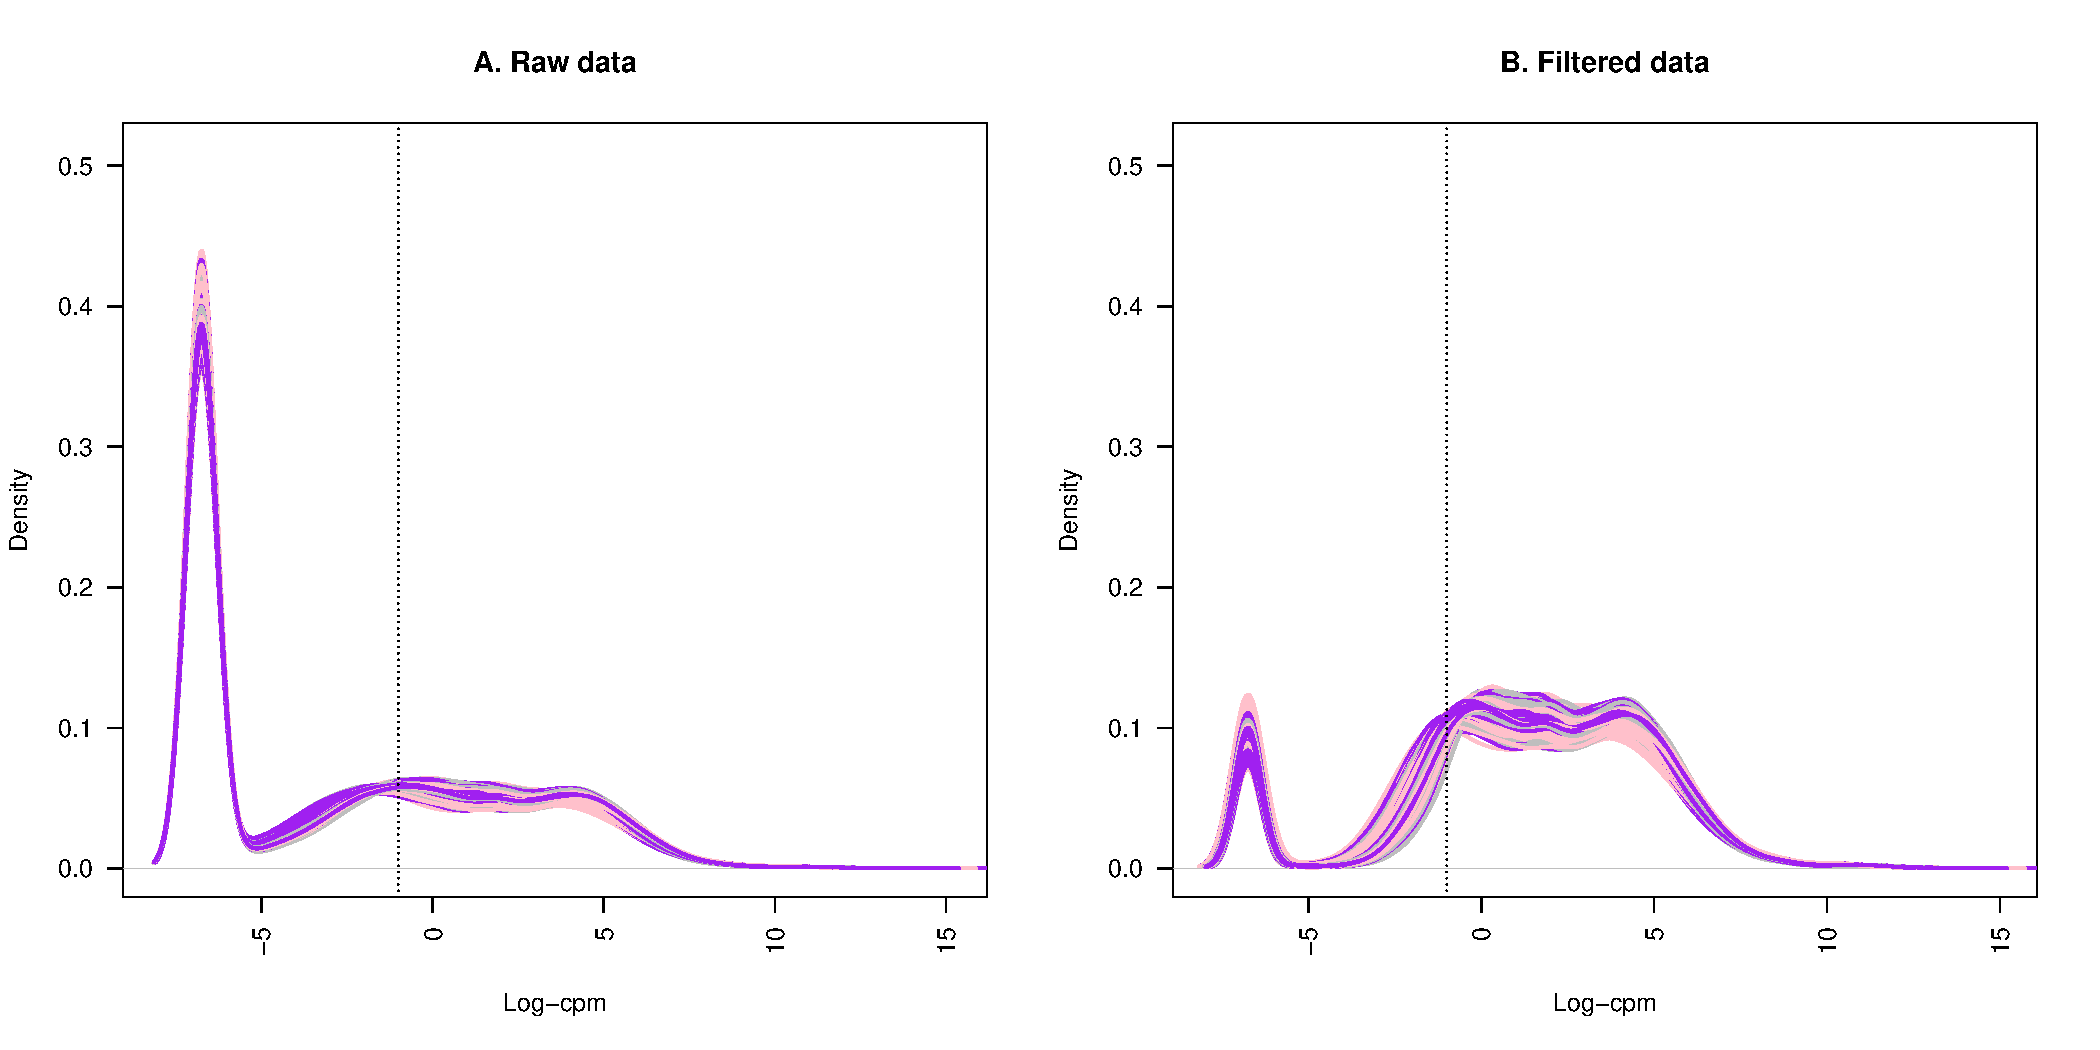
\includegraphics[width=1.0\textwidth]{mainmatter/figures/chapter_02/rnaseq_data_setup.sample_cpm_density_filtered.pdf}
    \caption{
        \textbf{Distributions of gene expression for \gls{RNAseq} samples before and after filtering low expression and non-detected genes.}
        Vertical line shows \gls{CPM} = 0.5 threshold.
    }
    \label{fig:hird_rnaseq_cpm_filtering}
\end{figure}

% 5.6.	Between-sample normalization of library size: Trimmed mean of M-values (TMM)
% Selecting between-sample RNA-Seq normalization methods from the perspective of their assumptions https://www.ncbi.nlm.nih.gov/pmc/articles/PMC6171491/
% 5.6.1.	edgeR::calcNormFactors generates norm.factors for each sample
%
% \1 NGS data is compositional, only quantifies relative abundance (without spike-ins of known conc)
%     https://academic.oup.com/gigascience/article/8/9/giz107/5572529
%     This property emerges from the sequencer itself; the sequencer, by design, can only sequence a fixed number of nucleotide fragments.
%     Consequently, the final number of fragments sequenced is constrained to an arbitrary limit so that doubling the input material does not double the total number of counts.
%     This constraint also means that an increase in the presence of any 1 nucleotide fragment necessarily decreases the observed abundance of all other transcripts [9], and applies to bulk and single-cell sequencing data alike.
%    It is especially problematic when comparing cells that produce more total RNA than their comparator (e.g., high–c-Myc cells, which up-regulate 90% of all transcripts without commensurate down-regulation [10]).
%     However, even if a sequencer could directly sequence every RNA molecule within a cell, the cells themselves are compositional because of the volume and energy constraints that limit RNA synthesis, as evidenced by the observation that smaller cells of a single type contain proportionally less total messenger RNA (mRNA) [11].
%     [..]
%     First, statistical models that assume independence between features are flawed because of the mutual dependency between components [15]. Second, distances between samples are misleading and erratically sensitive to the arbitrary inclusion or exclusion of components [16]. Third, components can appear definitively correlated even when they are statistically independent [17].
%     \2 raw abundance estimates are often called \enquote{counts}, but actually dimensionless proportions, interpretable only compared to other genes in the same sample (composition)
%     https://www.ncbi.nlm.nih.gov/pmc/articles/PMC6084572/
%     Compositional data measure each sample as a composition, a vector of non-zero positive values (i.e. components) carrying relative information (Aitchison, 1986).
%     Compositional data have two unique properties. First, the total sum of all component values (i.e. the library size) is an artifact of the sampling procedure (van den Boogaart and Tolosana-Delgado, 2008). Second, the difference between component values is only meaningful proportionally [e.g. the difference between 100 and 200 counts carries the same information as the difference between 1000 and 2000 counts (van den Boogaart and Tolosana-Delgado, 2008)].
%     \2 a fixed number of reads is sequenced: if a gene's counts go up, another will go down
%     https://rnajournal.cshlp.org/content/early/2020/04/13/rna.074922.120.full.pdf
%     \2 naive normalisations such as CPM, TPM, RPKM are still rates (per transcriptome), and cannot be compared across samples, as they still depend on composition
%     \2 normalisation such as TMM tries to account for composition by normalising on non DE genes, to allow for valid DGE analysis
%     \2 getting absolute measures is difficult without spike-ins
%     \2 for valid DGE, need to decide on the units e.g. mRNA/cell? mRNA/transcriptome? \autocite{soneson2013ComparisonMethodsDifferential}
%
\gls{RNAseq} produces compositional data due to sequencing a fixed number of reads per library; if one gene's expression goes up in a library, another's must go down.
In order for expression values to be comparable between different libraries (samples), it is important to account for composition bias: the dependence of expression estimates on the expression properties of other genes in each library \autocite{robinson2010ScalingNormalizationMethod}.
Effective library sizes were computed as between-sample normalisation factors using the \gls{TMM} method \autocite{robinson2010ScalingNormalizationMethod,evans2018SelectingBetweensampleRNASeq} from \software{edgeR::calcNormFactors} \autocite{robinson2010EdgeRBioconductorPackage}.
% NOTE: voom just does t(log2(t(counts + 0.5)/(lib.size + 1) * 1e+06)), where lib.size considers norm.factors, it does not variance-stabilise.
% The idea is to use precision weights for each observation instead.
%
% "Our strategy is to estimate non-parametrically the mean-variance trend of the logged read counts and to use this mean-variance relationship to predict the variance of each log-cpm value. The predicted variance is then encapsulated as an inverse weight for the log-cpm value. When the weights are incorporated into a linear modeling procedure, the mean-variance relationship in the log-cpm values is effectively eliminated."
% [...]
% "The standard deviation trend is then interpolated to predict the standard deviation of each individual observation based on its predicted count size (Figure 2c). Finally, the inverse squared predicted standard deviation for each observation becomes the weight for that observation."
Precision weights for each (gene by sample) observation were computed with \software{limma::voom} \autocite{law2014VoomPrecisionWeights} to account for the mean-variance relationship in \gls{RNAseq} data;
\software{limma::voom} also transforms expression values to the $\log_2{\text{\gls{CPM}}}$ scale using effective library sizes.

Finally, 15 samples were excluded for having missing \gls{HAI} or \gls{MN} data.
% From n=225-2 sequencing fails=223 (75/75 individuals on day 0, 73/75 on day 1, and 75/75 on day 7)
After the application of all filters, expression values were available for \num{21626} genes over 208 samples
(70/75 individuals on day 0, 68/75 on day 1, and 70/75 on day 7).

\subsection{Array data preprocessing}
\label{subsec:hird_dge_array_preproc}

% 6.	Pre-process microarray expression data
% 6.1.	Annotate Entrez and ENS ids using hgug4112a.db
% 6.1.1.	The chip is single-channel “Agilent-014850 Whole Human Genome Microarray 4x44K G4112F”. Scan_NumChannels is 1 in the raw files.
% 6.1.2.	Apparently fine to use 4112A db for 4112F https://support.bioconductor.org/p/73193/
% 6.2.	Redefine responder phenotype to be consistent with RNA-seq and Sobolev paper (>= 4-fold in HAI or MN)
% 6.3.	Background correction: limma::backgroundCorrect(x, method="normexp")
% 6.3.1.	Background comes from non-specific binding
% 6.3.2.	Pipeline from the Agi4x44PreProcess Bioconductor package (deprecated)
% 6.3.3.	Notes on Edwards: https://academic.oup.com/bioinformatics/article/23/20/2700/230165#2633725
% 6.3.3.1.	“adjusts the foreground intensities by subtracting the background when the difference between the foreground and background is larger than a small threshold value. When the difference is less than the threshold, subtraction is replaced by a smooth monotonic function.“
% 6.3.3.2.	May be preferred over normexp in our case due to “Question: Compressed boxplots after 'normexp+offset' background correction of Agilent one color microarrays in LIMMA“ https://support.bioconductor.org/p/46485/
% 6.3.3.3.	Example of Edwards used over normexp for Agilent arrays: “Modified least-variant set normalization for miRNA microarray” https://www.ncbi.nlm.nih.gov/pmc/articles/PMC2995391/
% 6.3.3.4.
% 6.3.4.	Notes on normexp:
% 6.3.4.1.	This function is designed to produce positive corrected intensities.
% 6.3.4.1.1.	“If the "normexp" method is selected, then a convolution of normal and exponential distributions is fitted to the foreground intensities using the background intensities as a covariate, and the expected signal given the observed foreground becomes the corrected intensity.”
% 6.3.4.1.2.	https://www.ncbi.nlm.nih.gov/pmc/articles/PMC2648902/ “A method normexp was introduced which models the observed intensities as the sum of exponentially distributed signals and normally distributed background values”
% 6.3.4.2.	[…] an offset value (normally 50) is used. This offset adds a constant to the intensities before log-transforming, so that the log ratios are shrunk towards zero at the lower intensities.
% 6.3.4.3.	The optimal choice for the offset is the one which makes the variability of the log-ratios as constant as possible across the range of intensity values (Smyth, G. in BioC mailing List, https://stat.ethz.ch/pipermail/bioconductor/2006-April/012554.html ).
% 6.3.5.	Choice of offset: https://academic.oup.com/nar/article/38/22/e204/1049223#93002104
% 6.3.5.1.	Adding an offset to the intensities before log transformation not only was found to lower the variance (improve precision) but also to compress the fold-change range and increase bias. In other words, offsets decrease noise but increase bias.
% 6.3.5.2.	The normexp by control (neqc) algorithm […] For routine practical use, we recommend modest offsets for Illumina data in the range of 10–50, which minimize the bias while still delivering a benefit in terms of FDR. Offsets of 16–50 have been used in a number of biological studies (10,13,16). These results remain essentially unchanged whether or not control probes are used […]  The default offset is 16, which seems generally to give good results on recent versions of human and mouse Illumina arrays.
% No need for normalizeWithinArrays in 2 color.
% 6.4.	Between-sample normalization: Limma::normalizeBetweenArrays(y, method="quantile")
% Why quantile normalise arrays? "A comparison of normalization methods for high density oligonucleotide array data based on variance and bias"
% 6.4.1.	Note that we omit any normalize within arrays procedures, as this is a single-channel array
% 6.4.2.	Normalization is the attempt to compensate for systematic technical differences between chips
% 6.4.3.	Uses https://www.rdocumentation.org/packages/limma/versions/3.28.14/topics/normalizeQuantiles
% 6.4.3.1.	“Each quantile of each column is set to the mean of that quantile across arrays. The intention is to make all the normalized columns have the same empirical distribution. This will be exactly true if there are no missing values and no ties within the columns: the normalized columns are then simply permutations of one another.”
% 6.4.4.	Also see this “StatQuest: Quantile Normalization” https://www.youtube.com/watch?v=ecjN6Xpv6SE
% 6.4.5.	This also does a log2 transform, so final units are normalized log2 intensity
%
Single-channel Agilent 4x44K expression array data (G4112F, 60-mer oligonucleotide probes) for 173 samples from \textcite{sobolev2016AdjuvantedInfluenzaH1N1Vaccination} were downloaded from ArrayExpress (\url{https://www.ebi.ac.uk/arrayexpress/experiments/E-MTAB-2313/}).
These arrays were originally processed in two batches, the effect of which can be seen in the raw foreground intensities (\cref{fig:hird_array_boxplots_raw}).

\begin{figure}
    \centering
    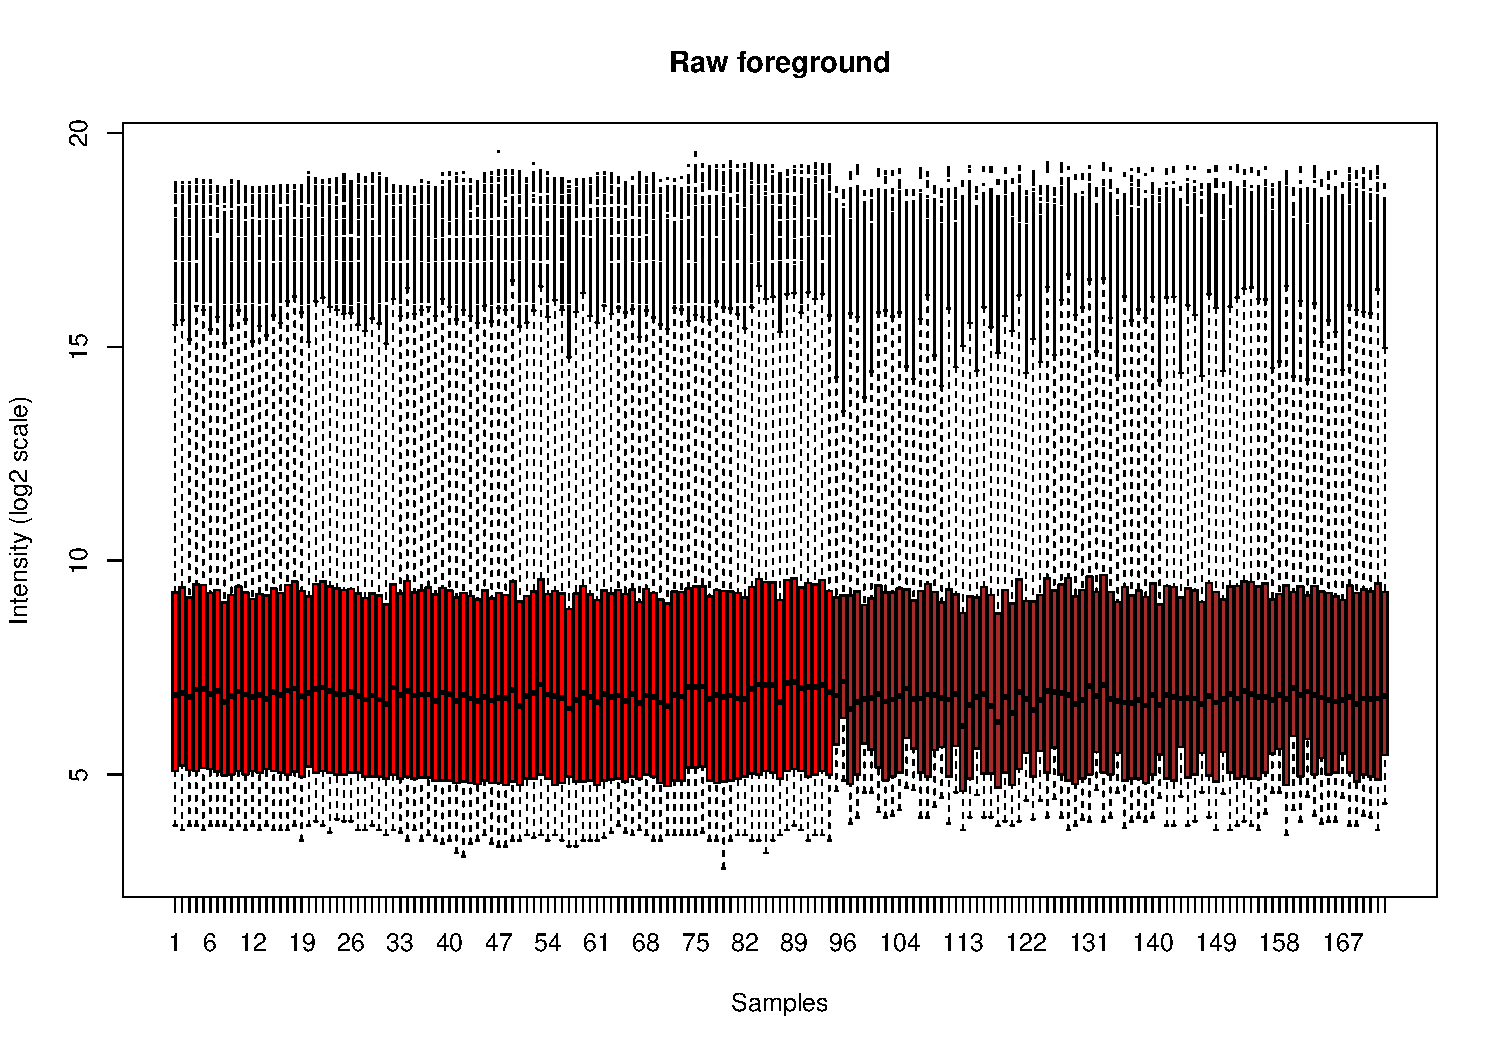
\includegraphics[width=1.0\textwidth,page=1]{mainmatter/figures/chapter_02/array_data_setup.array_intensity_boxplots.pdf}
    \caption{
        \textbf{Distribution of raw foreground intensities for 173 \gls{HIRD} array samples.}
        Colored by array processing batch.
    }
    \label{fig:hird_array_boxplots_raw}
\end{figure}

% TODO: why does array data have a mean-variance relationship?
% Standard statistical techniques often assume that data are normally distributed, with constant variance not depending on the mean of the data. Data that violate these assumptions can often be brought in line with the assumptions by application of a transformation. Gene-expression microarray data have a complicated error structure, with a variance that changes with the mean in a non-linear fashion.
% https://academic.oup.com/bioinformatics/article/18/suppl_1/S105/231903
%
% Note that the vsn algorithm performs background correction and normalization simultaneously.
% Does affine transformation, then glog2
% An affine transformation is simply a shifting and scaling of the data.
% The so-called glog2 (short for generalised logarithm) is a function that is like the logarithm (base 2) for large values (large compared to the amplitude of the background noise), but is less steep for smaller values.
\software{VSN::normalizeVSN} \autocite{huber2002VarianceStabilizationApplied} was used to simultaneously perform 
background correction, 
between-array normalisation (affine transformation, centers and scales each array to control for systematic experimental factors), 
and variance-stabilisation (generalised logarithm, similar to $\log_2$ with better performance for small values) of intensity values, 
resulting in expression values on a $\log_2$ scale.
As systematic experimental factors might differ between batches, requiring different centering and scaling factors, normalisation was performed per-batch, then the two batches were merged.

% 6.5.	Summarise probes (into loci): WGCNA::collapseRows(rowGroup=Ensembl ID, method="MaxMean", connectivityBasedCollapsing=FALSE)
% 6.5.1.	https://www.ncbi.nlm.nih.gov/pmc/articles/PMC3166942/
% 6.5.1.1.	“For example, we find that in most microarray experiments performed on brain tissue it is best to choose the probe with the maximum mean expression per gene, whereas when choosing a single gene to represent a co-expression module, the optimal collapsing method depends on the goal of the analysis.”
% 6.5.1.2.	“In the case of collapsing probes to their respective gene symbols, for example, we find that the 1.max strategy (implemented by setting method = "MaxMean" and connectivityBasedCollapsing = FALSE) produces the most robust results.”
% 6.5.1.3.	i.e. choose the probe with the highest mean of expression over the samples
Probes were matched to genes using \software{hgug4112a.db}\footnote{\url{https://bioconductor.org/packages/release/data/annotation/html/hgug4112a.db.html}}.
Most genes were targeted by multiple array probes; \num{31208} probes were collapsed into \num{18216} Ensembl genes using by selecting the probe with the highest mean intensity for each gene (\software{WGCNA::collapseRows(method = \enquote{MaxMean})}, recommended for probe to gene collapsing by \textcite{miller2011StrategiesAggregatingGene}).
While it would be optimal to select a collapsing method to maximise the concordance between array and \gls{RNAseq} expression values, there were no samples assayed by both platforms in the \gls{HIRD} dataset.
The final normalised $\log_2$ intensity values for these \num{18216} genes over 173 samples is shown in \cref{fig:hird_array_boxplots_MaxMean}.
% Also used arrayWeights as precision weight inputs to lmFit
% See: https://bmcbioinformatics.biomedcentral.com/articles/10.1186/1471-2105-7-261#Bib1
% The method successfully assigns lower weights to less reproducible arrays from different experiments. Down-weighting the observations from suspect arrays increases the power to detect differential expression.
Finally, \software{limma::arrayWeightsQuick} \autocite{ritchie2006EmpiricalArrayQuality} was used to compute per-sample quality weights used to downweight unreliable arrays (samples) in the \gls{DGE} analyses.

\begin{figure}
    \centering
    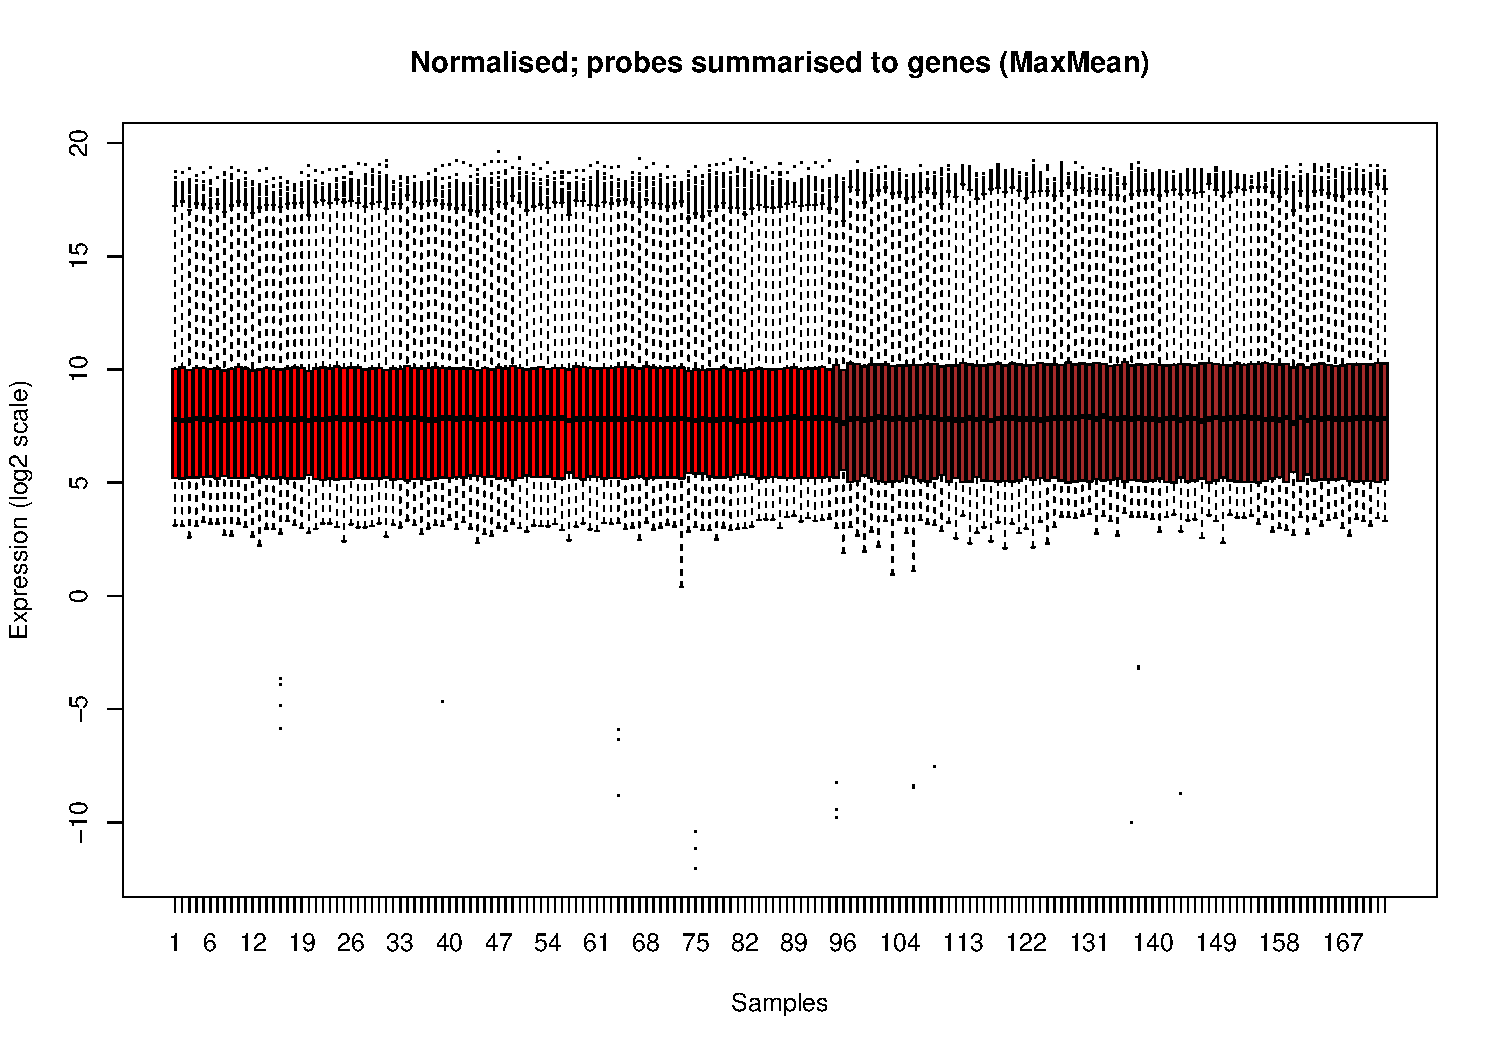
\includegraphics[width=1.0\textwidth]{mainmatter/figures/chapter_02/array_data_setup.array_intensity_boxplots.MaxMean.pdf}
    \caption{
        \textbf{Distribution of per-sample expression estimates after normalisation and collapsing of probes to genes.}
        Colored by array processing batch.
    }
    \label{fig:hird_array_boxplots_MaxMean}
\end{figure}

\subsection{\Glsfmtfull{DGE}}

\subsubsection{Platform and batch effects}
\label{subsubsec:hird_dge_platform_and_batch_effects}

Combining the normalised array and \gls{RNAseq} data resulted in expression values for \num{13593} genes assayed in both platforms for a total of 374 samples.
\gls{PCA} revealed that although samples separate by experimental timepoint along \gls{PC}3 (\cref{fig:hird_expression_pcs}e), 
measurement platform is by far the largest source of variation (\cref{fig:hird_expression_pcs}a).
Normalisation was also not able to completely remove the batch effect within the array data (\cref{fig:hird_expression_pcs}a).
The large platform effect likely stems from systematic technological differences in how each platform measures expression.
\gls{RNAseq} has a higher dynamic range, resulting less bias at low expression levels, but estimates are more sensitive to changes in depth than array estimates are to changes in intensity \autocite{robinson2015NestedParallelExperiment}.
Agreement between the two platforms is poor at extremes of expression \autocite{wang2009RNASeqRevolutionaryTool,ma2017JointBayesianModel}.
The preprocessing steps for the two platforms (\cref{subsec:hird_dge_rnaseq_quantAndFilter,subsec:hird_dge_array_preproc}) were also vastly different.

Despite the potential shortcomings of array data detailed above, the array dataset contains individuals with more extreme antibody response phenotypes (\cref{fig:hird_phenotypes_by_platform}), and hence should not be excluded.
Given the magnitude of the platform effect, I concluded that the appropriate approach was a two-stage approach that meta-analyses per-platform \gls{DGE} effect estimates while explicitly accounting for between-platform heterogeneity.

% TODO: 
% should you scale before PCA?
% https://github.com/matloff/regtools/blob/master/inst/ScalingInPCA.md?s=09
\begin{figure}
    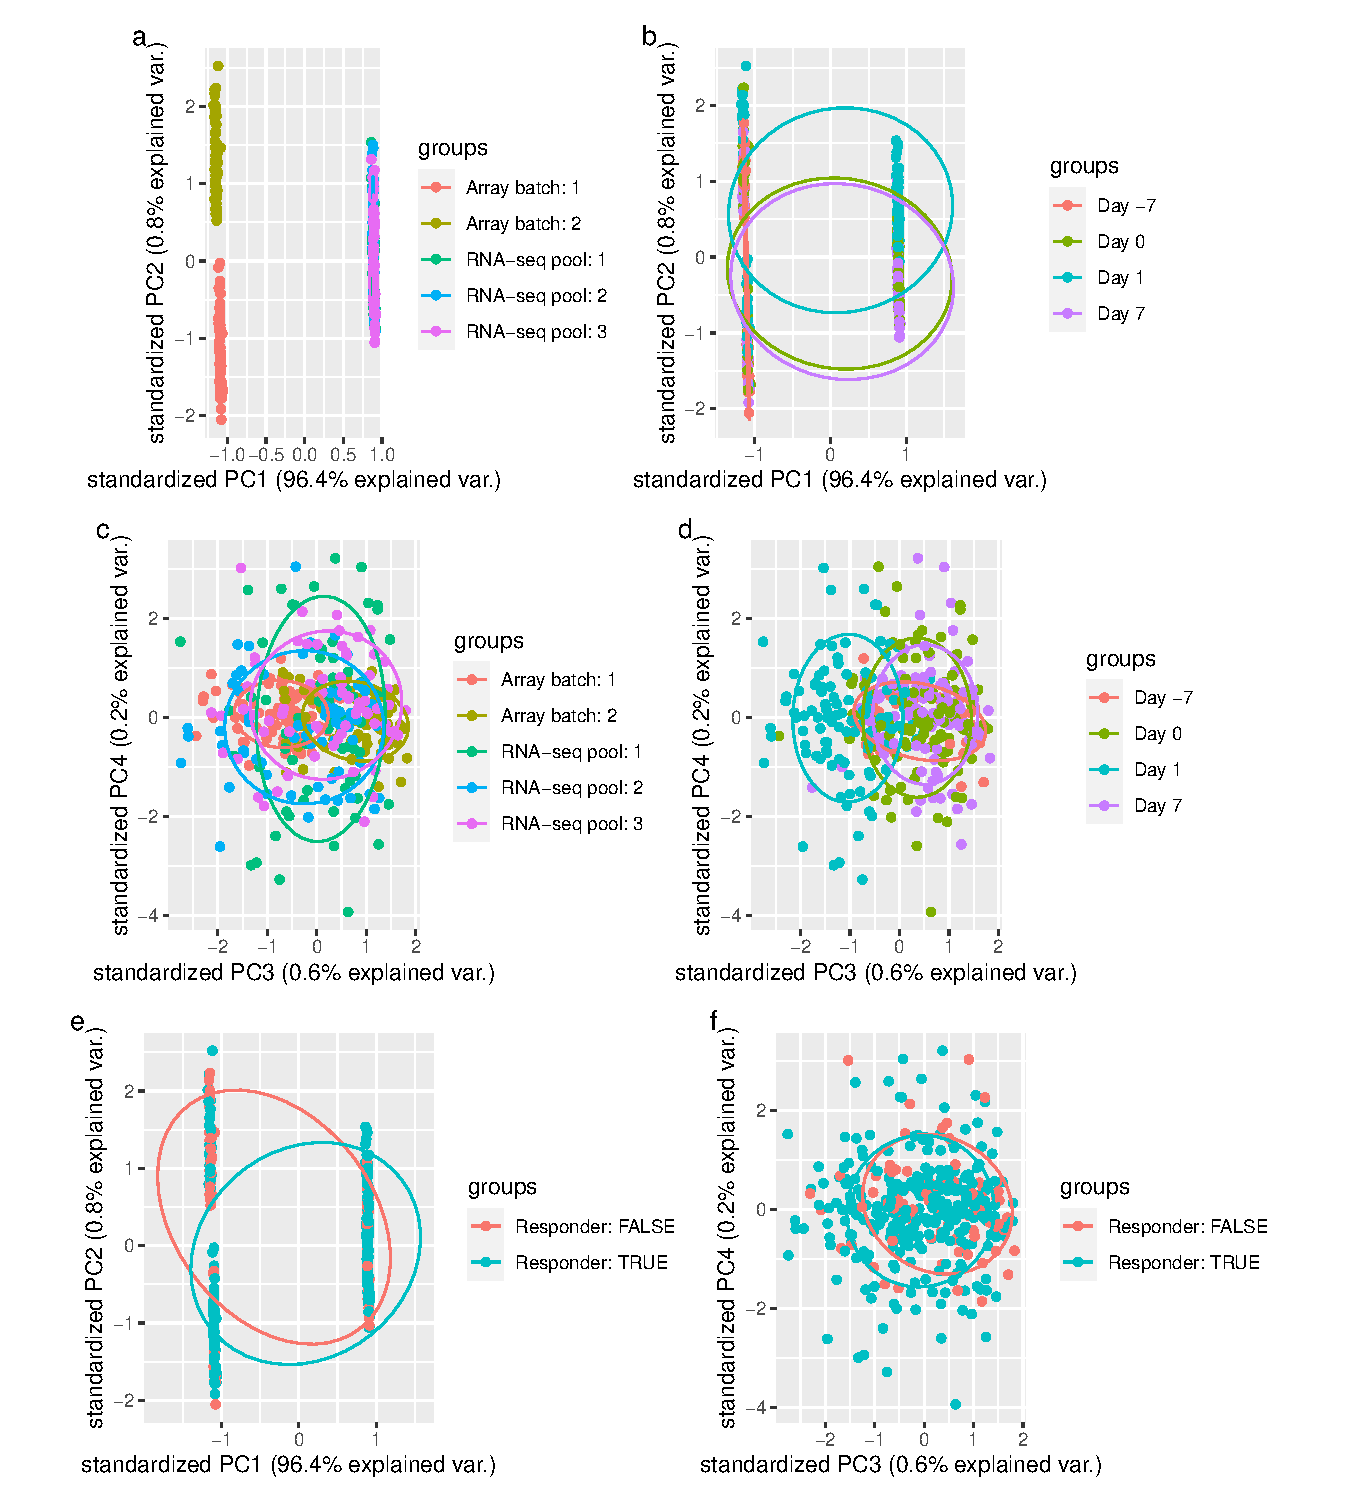
\includegraphics[width=1.0\textwidth,page=1]{mainmatter/figures/chapter_02/compare_phenotype_by_platform.E_pca.pdf}
    \caption{
        \textbf{First four standardised \glspl{PC} in the expression data, colored by array batch/\gls{RNAseq} pool (a, c), and timepoint (b, d) and binary response status (e, f).}
        Expression of each gene was standardised across samples within each platform before \gls{PCA}.
    }
    \label{fig:hird_expression_pcs}
\end{figure}

Regarding the batch effect within the array data, a popular adjustment method is ComBat \autocite{johnson2007AdjustingBatchEffects}, which estimates per-gene, per-batch centering and scaling parameters, which are shrunk towards the per-batch mean parameters over all genes using empirical Bayes to improve robustness.
ComBat was the method used by \textcite{sobolev2016AdjuvantedInfluenzaH1N1Vaccination}.
In comparisons of array batch effect adjustment methods, ComBat performed favourably (versus five other adjustment packages) \autocite{chen2011RemovingBatchEffects} or comparably (versus fitting batch as a fixed or random effect in the linear model, which are centering-only corrections) \autocite{espin-perez2018ComparisonStatisticalMethods}.
However, where batches are unbalanced in terms of sample size \autocite{zhang2018AlternativeEmpiricalBayes} or distribution of study groups that have an impact on expression \autocite{nygaard2015MethodsThatRemove}, ComBat can overcorrect batch differences or bias estimates of group differences respectively.
In our data, sample size and timepoint groups are fairly balanced between the two array batches (\cref{tab:hird_batch_balance}).
The proportion of responders is not, but response status does not have as prominent an impact on global expression as timepoint (\cref{fig:hird_expression_pcs}).
For the \gls{DGE} analyses in this chapter, I chose to model batches (array batch and \gls{RNAseq} pool) as fixed effects rather than pre-adjusting with Combat in a separate step, ensuring the \glspl{df} in the \gls{DGE} model were correct.
In practice, results from the analyses were not substantially affected by the choice of whether to use a ComBat pre-adjustment or a fixed effect.
%
% https://support.bioconductor.org/p/72815/ "batch effect : comBat or blocking in limma ?"
% In general, I would prefer to model batch effects by including them in the design matrix and modeling the unadjusted data. This ensures that the linear model properly accounts for the degress of freedom associated with modeling the batch effect, so that it uses the proper number of residual df. This prevents the linear model from overestimating significance because it thinks there are more residual df than there really are.

% NOTE: this table contains manual edits
\begin{table}[] 
 \centering 
 \caption[\captionshort{Distribution of \gls{HIRD} samples among timepoint and responder groups in the array batches and \gls{RNAseq} pools.}]{\textbf{Distribution of \gls{HIRD} samples among timepoint and responder groups in the array batches and \gls{RNAseq} pools.} Values are count and percentage for categorical variables; mean and standard deviation for continuous variables.}\label{tab:hird_batch_balance}
 \begin{tabular}{ l c c c c c c }
 \toprule
  &   &  \multicolumn{ 5 }{c}{ Array batch/\gls{RNAseq} pool }\\ 
  & Total & Array 1 & Array 2 & \gls{RNAseq} 1 & \gls{RNAseq} 2 & \gls{RNAseq} 3\\ 
  & n = 374 & n = 87 & n = 79 & n = 70 & n = 69 & n = 69 \\ 
  \midrule
 Day &   &   &   &   &   &  \\ 
 \hspace{6pt}    -7 & 40 (10.7\%) & 20 (23\%) & 20 (25.3\%) & 0 (0\%) & 0 (0\%) & 0 (0\%)\\ 
 \hspace{6pt}    0 & 114 (30.5\%) & 24 (27.6\%) & 20 (25.3\%) & 24 (34.3\%) & 23 (33.3\%) & 23 (33.3\%)\\ 
 \hspace{6pt}    1 & 109 (29.1\%) & 21 (24.1\%) & 20 (25.3\%) & 22 (31.4\%) & 23 (33.3\%) & 23 (33.3\%)\\ 
 \hspace{6pt}    7 & 111 (29.7\%) & 22 (25.3\%) & 19 (24.1\%) & 24 (34.3\%) & 23 (33.3\%) & 23 (33.3\%)\\ 
 Responder &   &   &   &   &   &  \\ 
 \hspace{6pt}    FALSE & 80 (21.4\%) & 12 (13.8\%) & 36 (45.6\%) & 11 (15.7\%) & 9 (13\%) & 12 (17.4\%)\\ 
 \hspace{6pt}    TRUE & 294 (78.6\%) & 75 (86.2\%) & 43 (54.4\%) & 59 (84.3\%) & 60 (87\%) & 57 (82.6\%)\\ 
 TRI &   &   &   &   &   &  \\ 
 \hspace{6pt}   & -0.1 (1.0) & -0.1 (1.0) & -0.4 (1.4) & 0.1 (0.6) & -0.0 (0.8) & 0.2 (0.6)\\ 
 \bottomrule
 
 \end{tabular}
 \end{table}


\subsubsection{Per-platform \glsfmtshort{DGE} model}
\label{subsubsec:hird_dge_per_platform_dge_model}

As a meta-analysis was performed, \gls{DGE} analyses were restricted to the \num{13593} genes assayed by both the array and \gls{RNAseq} platforms.
%
% 7.	Differential expression (limma)
% 7.2.	Create contrasts
% 7.3.	Estimate within-block correlation (duplicateCorrelation), using individuals as blocks
% 7.4.	Array data only: Compute sample quality weights for each array (arrayWeightsSimple(v, design=mod1))
% 7.5.	RNA-seq data only: Correct for mean-variance trend (voom)
% 7.5.1.	http://web.mit.edu/~r/current/arch/i386_linux26/lib/R/library/limma/html/voom.html
% 7.5.1.1.	“voom is an acronym for mean-variance modelling at the observational level. The key concern is to estimate the mean-variance relationship in the data, then use this to compute appropriate weights for each observation. Count data almost show non-trivial mean-variance relationships. Raw counts show increasing variance with increasing count size, while log-counts typically show a decreasing mean-variance trend. This function estimates the mean-variance trend for log-counts, then assigns a weight to each observation based on its predicted variance. The weights are then used in the linear modelling process to adjust for heteroscedasticity.”
% 7.5.1.2.	“voom performs the following specific calculations. First, the counts are converted to logCPM values, adding 0.5 to all the counts to avoid taking the logarithm of zero. The matrix of logCPM values is then optionally normalized. The lmFit function is used to fit row-wise linear models. The lowess function is then used to fit a trend to the square-root-standard-deviations as a function of average logCPM. The trend line is then used to predict the variance of each logCPM value as a function of its fitted value, and the inverse variances become the estimated precision weights.”
% 7.6.	(lmFit)
% 7.7.	(contrasts.fit)
% 7.8.	(eBayes/treat(robust=T))
% 7.8.1.1.1.	https://rdrr.io/bioc/limma/man/ebayes.html
% 7.8.1.1.1.1.	When lfc=0, treat is identical to eBayes, except that F-statistics and B-statistics are not computed.
% 7.8.1.1.2.	https://academic.oup.com/bioinformatics/article/25/6/765/251641 The TREAT fold-change threshold should be set to a low value below which no fold-change is likely to be of genuine interest. Researchers should be mindful that genes will need to exceed this threshold by some way, depending on the data, before being declared statistically significant. Our experience suggests a minimal value, such as a 10% fold-change, corresponding to τ=log2(1.1)=0.13 on the log2-scale. It would be better to interpret the threshold as ‘the fold-change below which we are definitely not interested in the gene’ rather than ‘the fold-change above which we are interested in the gene’.
% 7.9.	(decideTests)
Linear models were fit using \software{limma} \autocite{ritchie2015LimmaPowersDifferential}, 
which is computationally fast, 
performs well for sufficiently large ($n \ge 3$ per group) sample sizes \autocite{soneson2013ComparisonMethodsDifferential},
and internally considers the precision weights computed for \gls{RNAseq} observations in \cref{subsec:hird_dge_rnaseq_quantAndFilter},
and the array quality weights computed for array samples in \cref{subsec:hird_dge_array_preproc}.
As \textcite{sobolev2016AdjuvantedInfluenzaH1N1Vaccination} already found there was no global dissimilarity in array expression between day -7 and day 0,
for the \gls{DGE} analyses in this chapter, 
array day -7 and day 0 are treated as repeated measurements taken at a single \enquote{baseline} timepoint.

For each gene and platform, I fit a model (model 1) with expression as the response variable; 
with an intercept, timepoint (baseline, day 1, day 7), \gls{TRI}, array batch/\gls{RNAseq} pool, sex, age, and the first 4 genotype \glspl{PC} as fixed-effect predictors;
and individual as a random-effect predictor.
% NOTE:
% https://bioconductor.org/packages/release/bioc/vignettes/variancePartition/inst/doc/dream.html
% Limma has a built-in approach for analyzing repeated measures data using duplicateCorrelation(). The model can handle a single random effect, and forces the magnitude of the random effect to be the same across all genes.
% ...
% The duplicateCorrelation method estimates a single variance term genome-wide even though the donor contribution of a particular gene can vary substantially from the genome-wide trend.
Within-individual correlations for the random effect were estimated using \software{limma::duplicateCorrelation}.
A second model (model 2) was also fit, the only difference being two additional predictors for the multiplicative interactions between day 1 and day 7 with \gls{TRI}.
%
% See: https://stats.stackexchange.com/questions/151730/test-if-two-coefficients-are-statistically-different-in-logistic-regression
Model 1 was used for testing differences in expression between pairs of timepoints, and for testing association between \gls{TRI} and expression with timepoints pooled.
Model 2 was used for testing association between \gls{TRI} and expression at specific timepoints.
% TODO: add equations

Contrasts were defined, testing if linear combinations of estimated model coefficients are different from zero.
% TODO: What is a contrast? A contrast is essentially a difference in regression coefficients. We have seen that the regression coefficients can express a difference in means or a single mean, as well as the slope and intercept of a line. A contrast is a way of testing more general hypotheses about population means.
% A contrast is defined as the sum of each group mean multiplied by a coefficient for each group
% In statistics, particularly in analysis of variance and linear regression, a contrast is a linear combination of variables (parameters or statistics) whose coefficients add up to zero, allowing comparison of different treatments.[1][2]
%
From model 1, I defined contrasts for day 1 vs. baseline, day 7 vs. baseline, day 7 vs. day 1, \gls{TRI}, sex, and age.
For example, 
to test for association between \gls{TRI} and expression, 
    I used a contrast where
    the weight for the \gls{TRI} coefficient was 1,
    with all other coefficient weights set to 0;
to test for differences between day 7 vs. day 1,
    I used a contrast where
    the weight for the day 7 coefficient was 1,
    the weight for the day 1 coefficient was -1,
    and all other coefficient weights were 0.
From model 2, I defined contrasts for the \gls{TRI}, \gls{TRI}-day 1, and \gls{TRI}-day 7 interaction terms,
    which respectively test for association between \gls{TRI} and expression at specifically at baseline, day 1, and day 7.
%
% NOTE: moderated
% https://support.bioconductor.org/p/70175/
% es <- fit2$coefficients
% es_se <- sqrt(fit2$s2.post) * fit2$stdev.unscaled
Corresponding coefficients and standard errors for the contrasts were extracted from the \software{limma} models, 
which represent effect size in units of $\log_2$ expression fold change per unit change in predictor value.

\subsubsection{Choice of \glsfmtshort{DGE} meta-analysis method}
\label{subsubsec:hird_dge_meta_methodChoice}

% While there is abundant literature on single-platform (e.g. \autocite{tseng2012ComprehensiveLiteratureReview}) methods [...]
% TODO: add reasons why these don't solve the problem
%
% Examples from literature
%
% random effects:
%
% https://academic.oup.com/nar/article/45/17/9860/4084660#106485896
% - for example of REM of 24 array datasets
%
% Sweeney, T. E., Haynes, W. A., Vallania, F., Ioannidis, J. P., & Khatri, P. (2017). Methods to increase reproducibility in differential gene expression via meta-analysis. Nucleic Acids Research, 45(1), e1–e1. https://doi.org/10.1093/nar/gkw797
% - DGE random effects models should be possible with around 6-7 studies.
%
% SVA:
% Comparative RNA-Seq and Microarray Analysis of Gene Expression Changes in B-Cell Lymphomas of Canis familiaris
% https://www.ncbi.nlm.nih.gov/pmc/articles/PMC3617154/
% - applying SVA to our data revealed a strong correlation with known technical biases associated with RNA-Seq [26]–[28], [51] and removing the associated variation from the RNA-Seq samples resulted in the two technologies pairing by individual sample.
% - First, we have not attempted to capture differences in dynamic range between RNA-Seq and microarray. It is reasonable to expect that the larger dynamic range of RNA-Seq will result in larger variation. We found latent variation to be highly associated with GC content but, in contrast, found no clear evidence of an association pointing to nonlinear response in the microarrays. Second, the model underlying SVA does not explicitly capture different latent variables for the different technologies.
%
% MetaVolcano:
% The MetaVolcanoR R package combines differential gene expression results. It implements three strategies to summarize gene expression activities from different studies. i) Random Effects Model (REM) approach. ii) a vote-counting approach, and iii) a p-value combining-approach.
% - doesn't solve our small k problem
%
% CorMotif:
% https://academic.oup.com/biostatistics/article/16/1/31/259492
% - In contrast, a model that naively enumerates and analyzes all possible differential patterns across studies can deal with study-specificity and allow information pooling, but the complexity of its parameter space grows exponentially as the number of studies increases.
% - Here, we propose a correlation motif approach to address this dilemma. This approach searches for a small number of latent probability vectors called correlation motifs to capture the major correlation patterns among multiple studies.
% - First applies limma (Smyth, 2004) to each study separately. CorMotif is made for microarray data since it was motivated by the microarray analysis in the Sleep for Health in Hospital Programme (SHH) study. However, the idea behind CorMotif is general, and it should be straightforward to develop a similar framework for RNA-seq data.
% - designed for large k, seems similar to mashr
%
% CBM (“Cross-platform Bayesian Model”):
% - In this article, we propose a Bayesian hierarchical model to jointly integrate microarray and RNA-seq studies.
% - Since systematic fold change differences across RNA-seq and microarray for detecting differentially expressed genes have been previously reported, we replicated this finding in several real datasets and showed that incorporation of a normalization procedure to account for the bias improves the detection accuracy and power.
% - Cannot acually use CBM, as it operates on expressions, with a binary case vs control, so no covariates
%
% RankProd:
% - The Bioconductor package RankProd provides a new and intuitive tool for this purpose in detecting differentially expressed genes under two experimental conditions.
%
% Mayday seasight:
% - Uses a rank product model internally

Two popular frameworks for effect size meta-analysis are fixed-effect and random-effects \autocite{cohn2003HowMetaanalysisIncreases,borenstein2010BasicIntroductionFixedeffect}.
The fixed-effect model assumes a single true effect size $\theta$ common to all studies.
Given $k$ studies ($i = 1, \dots, k$), the observed effect size in the $i$th 
study is commonly assumed to be $y_i \sim \mathcal{N}(\theta,\sigma^2_i)$, where observed variation is explained only by within-study sampling error $\sigma_i$.
In meta-analysis, the effects are combined with some weighting, commonly the inverse variance (precision) $1/\sigma^2_i$.

The random-effects model assumes a distribution of true effects centered around a common mean $\mu$.
Each of the $k$ studies estimates its own study-specific true effect size $\theta_i$.
These are distributed around $\mu$ with variance $\tau^2$ (standard deviation $\tau$), representing an additional source of variation: the between-studies heterogeneity.
Then we have 
$y_i \sim \mathcal{N}(\theta_i,\sigma^2_i)$ for the first level of variation,
$\theta_i \sim \mathcal{N}(\mu,\tau^2)$ for the second level of variation,
and assuming these distributions, we have a normal-normal multilevel model \autocite{rover2017BayesianRandomeffectsMetaanalysis}.
Study weights include both within- and between-study variance $1/(\sigma^2_i + \tau^2)$, reducing to the fixed-effect model when $\tau=0$.

The choice of fixed or random effects depends on whether it is tenable to assume studies are identical enough that they all estimate a common effect% 
\footnote{
    A common misinterpretation is that random-effects meta-analysis assumes studies \emph{themselves} are sampled from a population of studies.
    This is rarely appropriate since the design of new studies is influenced by existing studies \autocite{higgins2009ReevaluationRandomeffectsMetaanalysis}.
    % Formally, a sequence is exchangeable if its joint probability distribution is a symmetric function of its n arguments.
    % Intuitively it means we can swap around, or reorder, variables in the sequence without changing their joint distribution.
    % https://stats.stackexchange.com/questions/3520/can-someone-explain-the-concept-of-exchangeability
    The required assumption is exchangability of study \emph{effects}, which informally states
    % IID (independent, identically distributed) -> exchangability -> identically distributed
    effects are neither completely identical nor completely independent, but \enquote{similar} \autocite{higgins2009ReevaluationRandomeffectsMetaanalysis}.
}.
In the \gls{HIRD} data, there are $k=2$ studies: array and \gls{RNAseq}.
The between-platform differences described in \cref{subsubsec:hird_dge_platform_and_batch_effects} represent considerable sources of between-study heterogeneity.
% NOTE: yuen2002AccuracyCalibrationCommercial, both oligonucleotide and cDNA arrays
For \gls{DGE} effect sizes, arrays also suffer from ratio compression of fold change estimates due to cross-hybridisation and probe saturation \autocite{yuen2002AccuracyCalibrationCommercial,draghici2006ReliabilityReproducibilityIssues,ma2017JointBayesianModel}.
The assumption of $\tau=0$ is unrealistic, so a random-effects model is more appropriate.

Unfortunately, there is no optimal solution for directly estimating $\tau$ in random-effects meta-analyses with small $k$ \autocite{bender2018MethodsEvidenceSynthesis}, and especially in the case of $k=2$ \autocite{gonnermann2015NoSolutionCombining}.
Many estimators are available \autocite{veroniki2016MethodsEstimateBetweenstudy}, but lack of information with small $k$ causes estimation to be imprecise, and often results in boundary values of $\tau = 0$ that are incompatible with the assumed positive heterogeneity \autocite{chung2013NondegeneratePenalizedLikelihood,friede2017MetaanalysisFewSmall}.
In such circumstances, the most sensible approach may be to incorporate prior information about hyperparameters $\mu$ and $\tau$ in a Bayesian random-effects framework \autocite{chung2013NondegeneratePenalizedLikelihood,veroniki2016MethodsEstimateBetweenstudy,friede2017MetaanalysisFewSmall,seide2019LikelihoodbasedRandomeffectsMetaanalysis}.
For this study, I used the implementation in \software{bayesmeta} \autocite{rover2017BayesianRandomeffectsMetaanalysis}.

\subsubsection{Prior for between-studies heterogeneity}

The choice of prior for between-studies heterogeneity $\tau$ is influential when $k$ is small \autocite{seide2019LikelihoodbasedRandomeffectsMetaanalysis}.
\textcite{gelman2006PriorDistributionsVariance} considers the case of $k=3$, showing that a flat prior places too much weight on implausibly large estimates of $\tau$, and recommends a weakly informative prior that acts to regularise the posterior distribution, constraining it away from implausible values.
%
% Gelman 
% - weak as in deliberately weaker than known knowledge, just serves to constrain
% - cauchy for the gentle slope in tails
% - also warns against inverse-gamma(e, e), as it can influence the posterior mean; it is not at all non-informative.
%
% Similarly, \autocite{friede2017MetaanalysisFewSmall} consider half-normals.
%
% More recent recommendations:
% \footnote{Documentation for Stan: \url{https://github.com/stan-dev/stan/wiki/Prior-Choice-Recommendations}.}
% - Gelman 2006 recommendations can actually be too weak for scale
% - Recommends Chung gamma(2, 1/A)
% - With full Bayes the boundary shouldn't be a problem (as long as you have any proper prior).
% - But with modal estimation, the estimate can be on the boundary, which can create problems in posterior predictions. For example, consider a varying-intercept varying-slope multilevel model which has an intercept and slope for each group. Suppose you fit marginal maximum likelihood and get a modal estimate of 1 for the group-level correlation. Then in your predictions the intercept and slope will be perfectly correlated, which in general will be unrealistic.
% Chung, Y., Rabe-Hesketh, S., Dorie, V., Gelman, A., & Liu, J. (2013). A Nondegenerate Penalized Likelihood Estimator for Variance Parameters in Multilevel Models. Psychometrika, 78(4), 685–709. https://doi.org/10.1007/s11336-013-9328-2
Since I assumed zero estimates for $\tau$ are unrealistic, I used a weakly informative gamma prior, as recommended by
\textcite{chung2013NondegeneratePenalizedLikelihood}, which has zero density at $\tau = 0$ but increases gently as $\tau$ increases (a positive constant derivative at zero).
This constrains $\tau$ to be positive, but still permits estimates close to zero if the data support it.
This is in contrast to priors used in other studies from the log-normal (e.g \autocite{pullenayegum2011InformedReferencePrior,turner2015PredictiveDistributionsBetweenstudy}) or inverse-gamma (e.g. \autocite{higgins1996BorrowingStrengthExternal}) families that have zero density at zero and derivatives of zero close to zero, ruling out small values of $\tau$ no matter what the data suggest; 
and in contrast to half-\textit{t} family priors (e.g. \autocite{gelman2006PriorDistributionsVariance,seide2019LikelihoodbasedRandomeffectsMetaanalysis}), which have their mode at zero, and do not rule out $\tau=0$.

Instead of constraining the value of $\tau$ for a gene's effect size to be a single unreliable estimate from $k=2$ data points,
assuming a prior distribution recognises that other genes may be informative of the range of plausible values for between-platform heterogeneity.
% rma.uni function
% By default, the starting value is set equal to the value of the Hedges (HE) estimator and the algorithm terminates when the change in the estimated value of \tau2 is smaller than 10^-5 from one iteration to the next.
To estimate the appropriate shape and scale parameters for the gamma empirically, 
a frequentist random-effects model using the \gls{REML} estimator for $\tau$ (recommended for continuous effects \autocite{veroniki2016MethodsEstimateBetweenstudy}) was fit for each gene using \software{metafor::rma.uni} \autocite{viechtbauer2010ConductingMetaAnalysesMetafor}.
Depending on the contrast, over half of resulting per-gene $\tau$ estimates were boundary values of zero.
Small estimates of $\tau < 0.01$ were excluded, and a gamma distribution fit to the remaining estimates using \software{fitdistrplus} \autocite{delignette-muller2015FitdistrplusPackageFitting}.

\subsubsection{Prior for effect size}

While the choice of prior on $\tau$ is influential when $k$ is small, there is usually enough data to estimate the effect size $\mu$ such that any reasonable non-informative prior can be used \autocite{gelman2006PriorDistributionsVariance,friede2017MetaanalysisFewSmall}.
% TODO why is this? is it having well powered studies? gelman is vague
\software{bayesmeta} implements both flat and normal priors for $\mu$.
%
% https://github.com/stan-dev/stan/wiki/Prior-Choice-Recommendations
% For example, it is common to expect realistic effect sizes to be of order of magnitude 0.1 on a standardised scale (for example, an educational innovation that might improve test scores by 0.1 standard deviations). In that case, a prior of N(0,1) could be considered very strong, in that it puts most of its mass on parameter values that are unrealistically large in absolute value. When we say this prior is "weakly informative," what we mean is that, if there's a reasonably large amount of data, the likelihood will dominate, and the prior will not be important. If the data are weak, though, this "weakly informative prior" will strongly influence the posterior inference. The phrase "weakly informative" is implicitly in comparison to a default flat prior.
% Weakly informative prior should contain enough information to regularize: the idea is that the prior rules out unreasonable parameter values but is not so strong as to rule out values that might make sense
% Weakly informative rather than fully informative: the idea is that the loss in precision by making the prior a bit too weak (compared to the true population distribution of parameters or the current expert state of knowledge) is less serious than the gain in robustness by including parts of parameter space that might be relevant. It's been hard for us to formalize this idea.
% One principle: write down what you think the prior should be, then spread it out. The idea is that the cost of setting the prior too narrow is more severe than the cost of setting it too wide. I've been having trouble formalizing this idea.
% Don't use uniform priors, or hard constraints more generally, unless the bounds
% represent true constraints (such as scale parameters being restricted to be
% positive, or correlations restricted to being between -1 and 1).
Assuming that most genes are not differentially expressed with effect sizes distributed randomly around zero, I selected a normal prior with $N(\mu=0, \sigma^2)$, over a flat prior. As in the section above, to determine an appropriate scale, a normal distribution with mean $\mu = 0$ was fit to the distribution of effect sizes from the per-gene frequentist models to empirically estimate $\sigma$.

% Another Cauchy example:
% Gelman, A., Jakulin, A., Pittau, M. G., & Su, Y.-S. (2008). A weakly informative default prior distribution for logistic and other regression models. The Annals of Applied Statistics, 2(4), 1360–1383. https://doi.org/10.1214/08-AOAS191
% - Cauchy 2.5
Heavy-tailed Cauchy priors have been proposed for effect size distributions in \gls{DGE} experiments to avoid over-shrinkage of true large effects in the tails \autocite{zhu2019HeavytailedPriorDistributions}.
Since \software{bayesmeta} does not implement a Cauchy prior, to avoid over-shrinkage, I flatten the normal prior considerably by scaling up the standard deviation by a factor of 10: $N(0, (10\sigma)^2)$.
This places a \SI{95}{\percent} prior probability that effects are less extreme than approximately 20 times the observed $\sigma$, sufficient to allow for extreme fold-changes.
% NOTE:
% The derivation here is qnorm(0.975, mean=0, sd=sqrt(100*1)) = 1*19.59964
% Alternatively: pnorm(19.59964, mean=0, sd=sqrt(100*1)) - pnorm(-19.59964, mean=0, sd=sqrt(100*1)) = 0.95

\subsubsection{Example of priors}

An example of the empirically estimated hyperparameters for the priors for the day 1 vs. baseline contrast are shown in \cref{fig:hird_dgeMeta_priors_tau} (for $\tau$) and \cref{fig:hird_dgeMeta_priors_mu} (for $\mu$).
For $\tau$, the final prior used was $\text{Gamma}(\text{shape}=\num{1.5693}, \text{scale}=\num{0.0641})$.
This is comparable to the default recommendation from \textcite{chung2013NondegeneratePenalizedLikelihood} of a $\text{Gamma}(\text{shape}=2, \text{scale}=\lambda)$ prior where $\lambda$ is small.
% TODO: add table with priors for all contrasts
For $\mu$, the final prior used was $N(0, (0.324 \times 10)^2)$.
The tails of the non-scaled normal fit (black) are light compared to the Cauchy fit (red), which may lead to over-shrinkage, especially since there are many genes with high positive fold changes for the day 1 vs. baseline effect.

\begin{figure}
    \includegraphics[width=1.0\textwidth,page=2]{mainmatter/figures/chapter_02/meta.bayesmeta.priors.coefName_d1.vs.d0.pdf}
    \caption{
        \textbf{Gamma prior for $\tau$ (blue) used for \software{bayesmeta} analyses of the day 1 vs. baseline effect, compared to the empirical distribution of per-gene frequentist \software{metafor::rma.uni} estimates for $\tau$.}
        Genes with small estimates of $\tau < 0.01$ were excluded before distribution fitting.
        Empirical log-normal fit also shown (red).
        Distribution parameters are listed.
    }
    \label{fig:hird_dgeMeta_priors_tau}
\end{figure}

\begin{figure}
    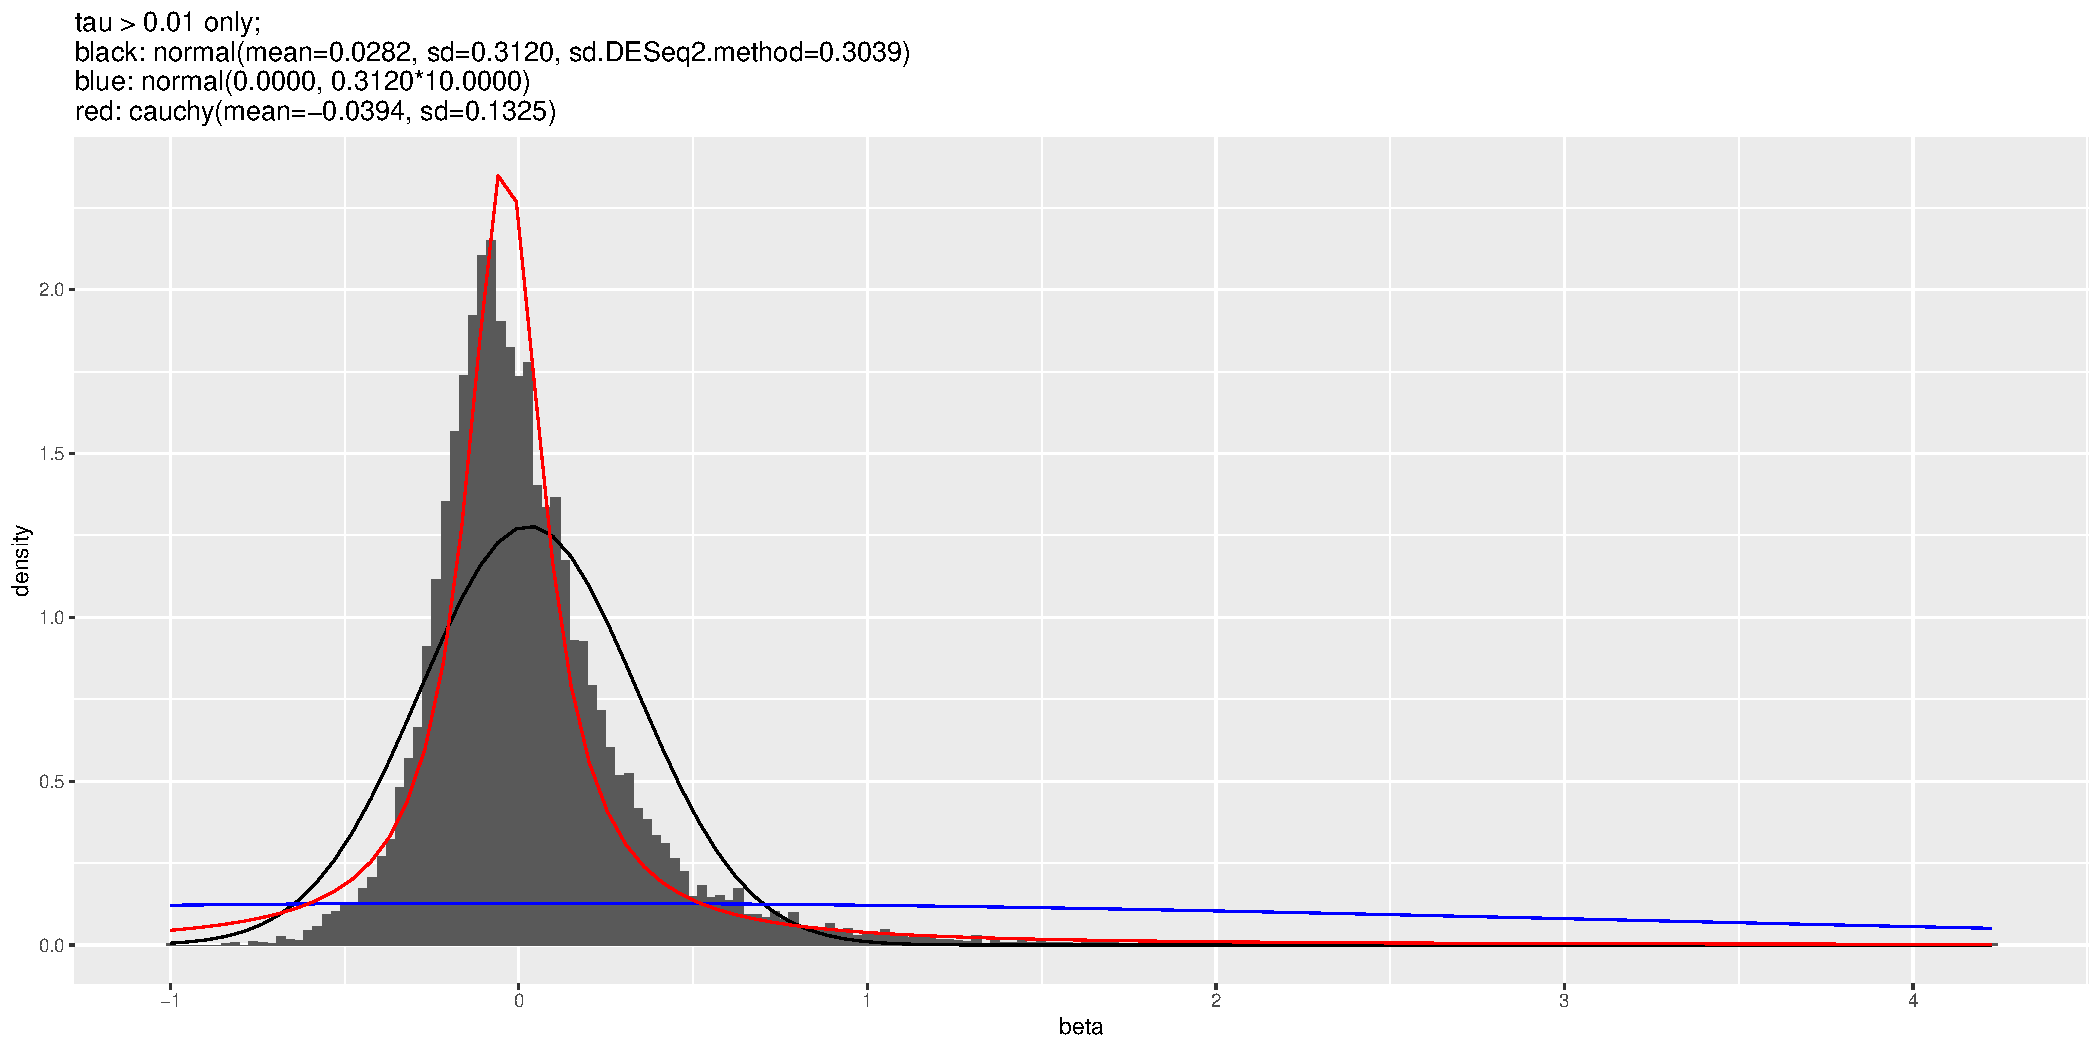
\includegraphics[width=1.0\textwidth,page=1]{mainmatter/figures/chapter_02/meta.bayesmeta.priors.coefName_d1.vs.d0.pdf}
    \caption{
        \textbf{Normal prior for $\mu$ (blue) used for \software{bayesmeta} analyses of the day 1 vs. baseline \gls{DGE} effect, compared to the empirical distribution of per-gene frequentist \software{metafor::rma.uni} estimates for $\tau$.}
        Genes with small estimates of $\tau < 0.01$ were excluded before distribution fitting.
        The original non-scaled normal fit is shown (black), as well as a Cauchy fit (red).
        Distribution parameters are listed.
        Alternative estimate of the Normal standard deviation more robust to outliers using a quantile matching method from \software{DESeq2} \autocite{love2014ModeratedEstimationFold} is also shown.
        In this case, it was comparable to the \gls{ML} estimate from \software{fitdistrplus}.
    }
    \label{fig:hird_dgeMeta_priors_mu}
\end{figure}

\subsubsection{Multiple testing correction}
\label{subsubsec:hird_dge_multipleTestingCorrection}

% The false discovery rate (FDR) is a method of conceptualizing the rate of type I errors in null hypothesis testing when conducting multiple comparisons. FDR-controlling procedures are designed to control the expected proportion of "discoveries" (rejected null hypotheses) that are false (incorrect rejections of the null).[1] FDR-controlling procedures provide less stringent control of Type I errors compared to familywise error rate (FWER) controlling procedures (such as the Bonferroni correction), which control the probability of at least one Type I error.
%
% NOTE: FDR BH assumes:
% "One assumption of the usual method is that the set of comparisons are either independent or have "Positive dependency""
% https://stats.stackexchange.com/questions/111756/the-meaning-of-positive-dependency-as-a-condition-to-use-the-usual-method-for
For per-platform \gls{DGE}, \gls{FDR} was controlled with \software{limma::decideTests} using the \gls{BH} procedure.
For the frequentist random-effects meta-analysis, nominal per-gene \pvalues{} were converted to \gls{FDR} estimates using \software{p.adjust(method = \enquote{BH})} in R.
%
% There is no simple way to get p values from bayesmeta.
% Posterior predictive checks are implemented in the pppvalue() to generate pvalues by MCMC.
% Do not confuse with ma05$pposterior(mu=0), which is evaluation of the posterior distribution at a particular value.
For the Bayesian random-effects meta-analysis, 
the effect sizes and standard errors from the per-gene meta-analysis output from \software{bayesmeta} were supplied to \software{ashr} \autocite{stephens2016FalseDiscoveryRates},
which models the distribution of effects under the assumption of unimodality.
% TODO: what about symmetry?
\software{ashr} applies empirical Bayes shrinkage to improve the accuracy of effect estimation (e.g. against winner's curse),
returning posterior effect sizes, posterior standard errors, and their significance (\gls{lfsr}).
\gls{lfsr} is analogous to \gls{FDR}, but quantifies the probability, given the data, of calling the wrong sign for an effect,
rather than the confidence of a non-zero effect \autocite{stephens2016FalseDiscoveryRates}.
% "Of course, being confident in the sign of an effect logically implies that we are confident it is non-zero ..."
Unless otherwise stated, \gls{FDR} and \gls{lfsr} were controlled at the \SI{5}{\percent} level separately for each contrast,
as control is for the proportion of positives expected to be false positives,
which is scalable to multiple contrasts.
% NOTE: see "13.3    Multiple Testing Across Contrasts", limma usersguide.pdf

\subsection{Ranked gene set enrichment using \glsfmtlongpl{BTM}}
\label{subsec:hird_dge_geneSetEnrichment}

% Other sets
% TODO: can also add MSigDB hallmark sets, which include interferon sets; and of course gene ontology sets

The gene sets used were \glspl{BTM} from \textcite{chaussabel2008ModularAnalysisFramework} (prefixed \enquote{DC}) and \textcite{li2013MolecularSignaturesAntibody} (prefixed \enquote{LI}).
Modules are sets of genes with transcriptional and functional similarities across a variety of healthy, diseased, and stimulated conditions.
The 260 modules from \textcite{chaussabel2008ModularAnalysisFramework} were constructed by unsupervised clustering of 239 \gls{PBMC} transcriptomes from multiple disease datasets,
then annotated by data mining of gene names in PubMed abstracts.
The 334 modules from \textcite{li2013MolecularSignaturesAntibody} were constructed from coexpression analysis of approximately \num{30000} blood transcriptomes,
then annotated making use of \gls{GO} terms, cell type-specific markers, pathway databases, and manual literature searches.
These datasets are particularly suitable for systems vaccinology studies, given their focus on the blood transcriptome.
\textcite{li2013MolecularSignaturesAntibody} modules are better annotated in general, and were used for the majority of gene set enrichments in this chapter.

% FDR
% A data frame with module names, additional statistic (e.g. enrichment or AUC, depending on the test), P value and FDR q-value (P value corrected for multiple testing using the p.adjust function and Benjamini-Hochberg correction.
Gene set enrichment analyses were conducted using \software{tmod::tmodCERNOtest} \autocite{weiner3rd2016TmodPackageGeneral}, 
which assesses the enrichment of small ranks within specific sets of genes compared to all genes, after the genes are ranked by some metric---here I used effect sizes from \software{bayesmeta}.
%
% TODO
% More sophisticated ranking methods
% - tmodLimmaTest: The ordering of the genes according to a certain metric is the fundament for gene enrichment analysis. tmodLimmaTest allows three orderings: p-values, "MSD" and log fold changes. The default MSD ("minimal significant difference") is the lower boundary of the 95confidence interval for positive log fold changes, and 0 minus the upper boundary of the 95better than ordering by p-value or by log fold change. See discussion in the package vignette.
% - Minimum Significant Difference \url{https://link.springer.com/article/10.1186/s12859-017-1674-0#Abs1} \url{https://cran.r-project.org/web/packages/tmod/vignettes/tmod.pdf}
% - treat method \url{http://web.mit.edu/~r/current/arch/i386_linux26/lib/R/library/limma/html/ebayes.html}
% - camera is developed to use mod t
% - equivalence testing
%
The CERNO statistic for a gene set is:
\begin{equation}
    -2 \sum_{i=1}^{n} \ln \frac{r_i}{N} \sim \chi^2(2n)
\end{equation}
where $n$ is the number of genes in the set,
$N$ is the number of measured genes in the experiment,
% NOTE: depends on if filter=T is set in tmod::tmodCERNOtest and evidencePlot
% (the size of the intersection between genes in the experiment and genes in the set of \glspl{BTM} used),
and $r_i \in 1, 2, ..., N$ is the rank of the $i$th gene in the set among all measured genes.
CERNO is relatively robust to the ranking metric \autocite{zyla2019GeneSetEnrichment}.
\gls{FDR} control for the number of gene sets tested was performed using \gls{BH}, again separately for each contrast.
% TODO: consider global correction, if the aim is to identify which day is most associated
The $\chi^2$ test is one-sided, so \software{tmod::tmodCERNOtest} only considers enrichment of small ranks when computing significance.
As genes can be down or upregulated, 
separate tests were performed sorting genes in ascending and descending order,
and the more significant result was used to determine the overall direction of effect for each gene set.
As the approach is rank-based and considers all measured genes, no filters based on the ranking metric were necessary.

The effect size of a gene set enrichment can be quantified with the \gls{AUC},
computed from $U$, the test statistic from a Mann-Whitney U test (also known as the Wilcoxon rank-sum test):
\begin{equation}
    U = n(N-n) + \frac{n(n + 1)}{2} - \sum_{i=1}^{n} r_i
\end{equation}
This is a non-parametric test for whether genes in the set have smaller ranks than genes not in the set on average.
Then $\text{\gls{AUC}} = U/(n(N-n))$, which takes values from 0 to 1.
Significant results from the one-sided \software{tmod::tmodCERNOtest} will always have $\text{\gls{AUC}} > 0.5$.
%
% NOTE: from the tmod::tmodCERNOtest code:
%
% l is the sorted list of genes, N is the total number of genes
%     N <- length(l)
%     x <- l %in% mset$MODULES2GENES[[m]]
% N1 is the number of genes in the module
%     N1 <- sum(x)
% ranks are the ranks of genes in the module
%     ranks <- c(1:N)[x]
% cerno is -2 * sum of the log fractional ranks of genes in the module
%     cerno <- -2 * sum(log(ranks/N))
% cES is CERNO scaled by the module size
%     cES <- cerno/(2 * N1)
% R1 is the rank sum of genes in the module
%     ret <- c(cerno = cerno, N1 = N1, R1 = sum(ranks), cES = cES, P.Value = 1)
% N2 is number of genes not in the module
%     N2 <- N - N1
% U statistic  
%     R1 <- ret$R1
%     U <- N1 * N2 + N1 * (N1 + 1)/2 - R1
% AUC scales U by N1 * N2
%     ret$AUC <- U/(N1 * N2)
%     ret <- ret[, c("cerno", "N1", "AUC", "cES")]
% P.value comes from comparing CERNO against chi2 with 2 * N1 df
%     ret$P.Value = pchisq(ret$cerno, 2 * ret$N1, lower.tail = FALSE)

\section{Results}

\subsection{Extensive global changes in expression after vaccination}

To gain an overview of how the transcriptome changes after vaccination, linear models were fit to identify genes differentially expressed at day 1 or day 7 compared to baseline (day -7 and day 0) in the \gls{HIRD} array and \gls{RNAseq} expression data, accounting for covariates such as batch effects, sex, age, \gls{TRI}, and ancestry.
At the \num{13593} genes with expression measured by both platforms, models were fit within each platform.
A frequentist random-effects meta-analysis was initially run to generate plausible values for \gls{DGE} effect size and between-platform heterogeneity.
These were used to form empirical priors for a Bayesian random-effects meta-analysis, producing final posterior estimates of effect size and standard errors.

Vaccination induced changes in a large proportion of the \gls{PBMC} transcriptome; \num{6257/13593} genes were differentially expressed between any pair of timepoints ($\text{\gls{lfsr}} < 0.05$).
Applying an absolute $\text{\gls{FC}} > 1.5$ cutoff identified 857 genes with the strongest effects.
Their expression clustered into three general patterns:
    upregulation from baseline to day 1, then downregulation from day 1 to day 7 back to baseline levels;
    upregulation from baseline to day 1, sustained at day 7; 
    and downregulation from baseline to day 1, then upregulation from day 1 to day 7 back to baseline levels (\cref{fig:hird_dge_heatmap}).
%
%               sign
% coef.name   -1   1
%   d1.vs.d0  64 580
%   d7.vs.d0   0  59
%   d7.vs.d1 679 140
 
\begin{figure}
    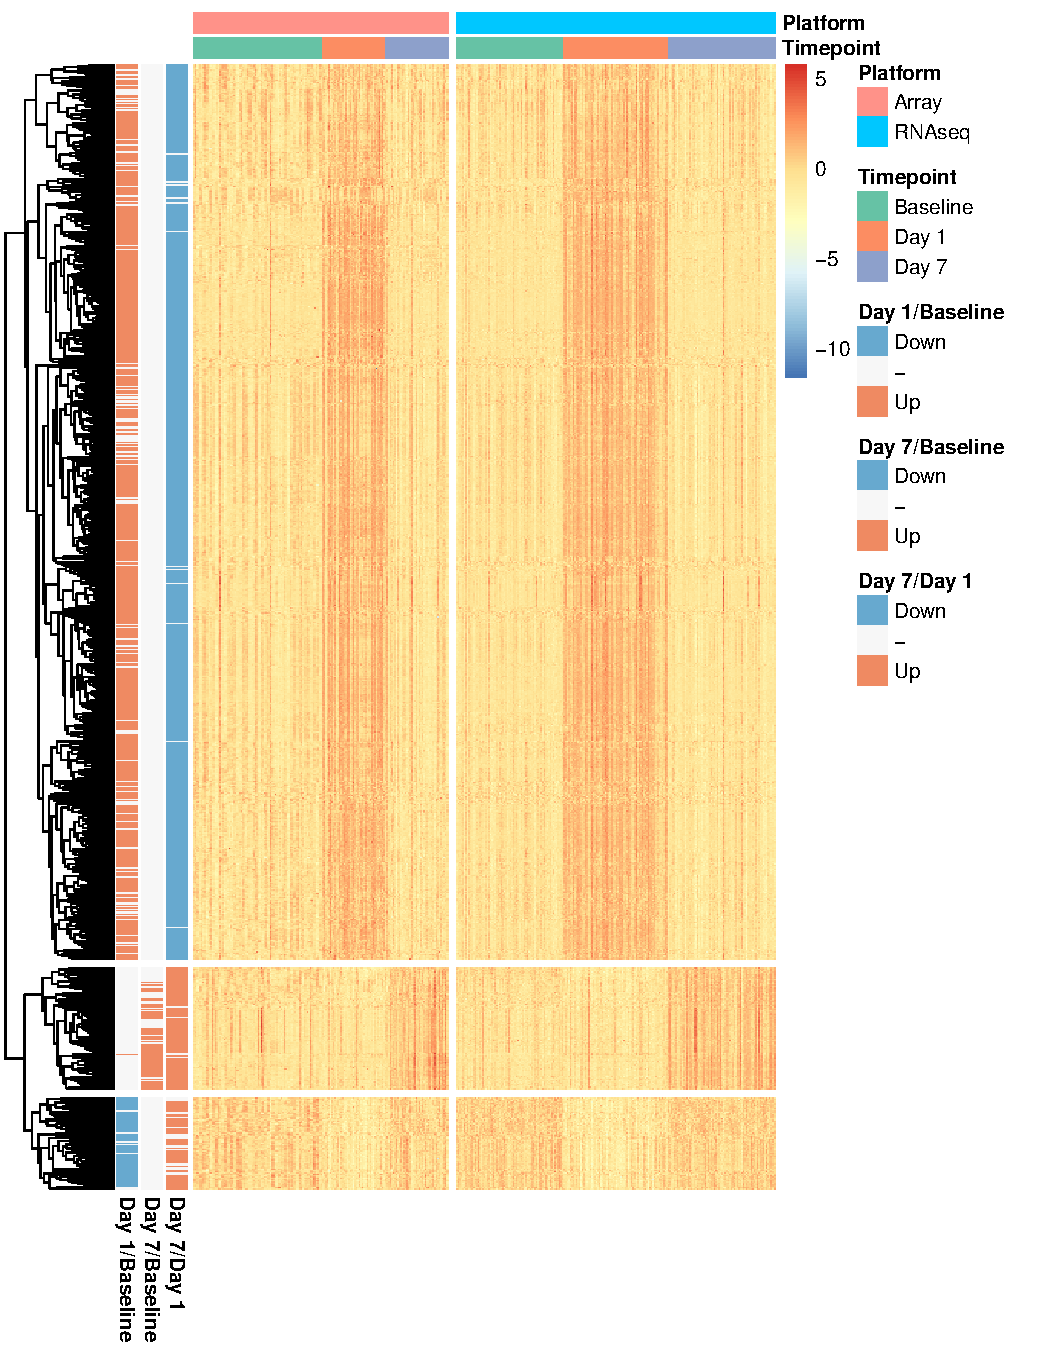
\includegraphics[width=1.0\textwidth]{mainmatter/figures/chapter_02/plot_dge_eqtl.heatmap_dge.pdf}
    \caption{
        \textbf{Normalised gene expression for 857 genes differentially expressed between any pair of timepoints ($\text{lfsr} < 0.05$, $\lvert\text{\gls{FC}}\rvert > 1.5$).}
        Rows are genes; columns are samples.
        Genes were standardised within-platform, then hierarchically-clustered by Manhattan distance.
        Baseline timepoints are days -7 and 0.
        Row annotations show \gls{DGE} between pairs of timepoints.
        Column annotations show sample platform and timepoint.
    }
    \label{fig:hird_dge_heatmap}
\end{figure}

\subsubsection{Innate immune response at day 1 post-vaccination}

Consistent with global expression at day 1 being markedly different from expression at other timepoints (\cref{fig:hird_expression_pcs}), the highest numbers of differentially expressed genes were observed at day 1, with 644 genes differentially expressed vs. baseline.
The majority of these (580/644) were upregulated.
The gene with the highest \gls{FC} increase at day 1 compared to baseline was \gene{ANKRD22} ($\log_2\text{\gls{FC}} = \num{4.489150}$), an interferon-induced gene in monocytes and \glspl{DC} involved in antiviral innate immune pathways \autocite{bin2016AnkyrinRepeatDomain}.
Other key genes in the interferon signalling pathway \autocite{schneider2014InterferonStimulatedGenesComplex} such as \gene{STAT1} ($\log_2\text{\gls{FC}} = \num{2.1693060}$), \gene{STAT2} ($\log_2\text{\gls{FC}} = \num{0.9489341}$), and \gene{IRF9} ($\log_2\text{\gls{FC}} = \num{0.8153674}$) were also upregulated at day 1.
% TODO: add module names and FDRs
Rank-based gene set enrichment analysis using \software{tmod} \autocite{weiner3rd2016TmodPackageGeneral} revealed that genes with the large \gls{FC} increases at day 1 were enriched in modules associated with interferon, activated \glspl{DC}, monocytes, and \glspl{TLR} and inflammatory signalling (\cref{fig:hird_tmodDotPlot_timepoint}).
\textcite{sobolev2016AdjuvantedInfluenzaH1N1Vaccination} reported only a 1.6-fold ($\log_2 1.6 = \num{0.6780719}$) increase in blood monocytes from baseline to day 1, as measured by \gls{FACS}, so these changes reflect active, per-cell upregulation as well as proliferation.

Sixty-four genes were downregulated at day 1, enriched in modules associated with T cells and \gls{NK} cells.
The largest absolute fold change was observed for \gene{FGFBP2} ($\log_2\text{\gls{FC}} = \num{-0.9141547}$), 
which encodes Ksp37, a secretory protein unique to CD8\textsuperscript{+} T cells and \gls{NK} cells \autocite{ogawa2001NovelSerumProtein}.
Again, the fold changes in expression were of greater magnitude than observed for the abundance of these cell types, suggesting active downregulation \textcite{sobolev2016AdjuvantedInfluenzaH1N1Vaccination}.

As can be seen in \cref{fig:hird_dge_heatmap}, there was a general tendency for expression to return to baseline levels by day 7.
This was the case for 566/644 upregulated genes and 44/64 downregulated genes,
indicating the innate phase of response likely peaks in the first few days.
%   d1.vs.d0 d7.vs.d0 d7.vs.d1 count
%      <dbl>    <dbl>    <dbl> <int>
% 1       -1       NA        1    44
% 2       -1       NA       NA    20
% 3        1        1       NA     1
% 4        1       NA       -1   566
% 5        1       NA       NA    13
% 6       NA        1        1    54
% 7       NA        1       NA     4
% 8       NA       NA       -1   113
% 9       NA       NA        1    42

\begin{figure}
    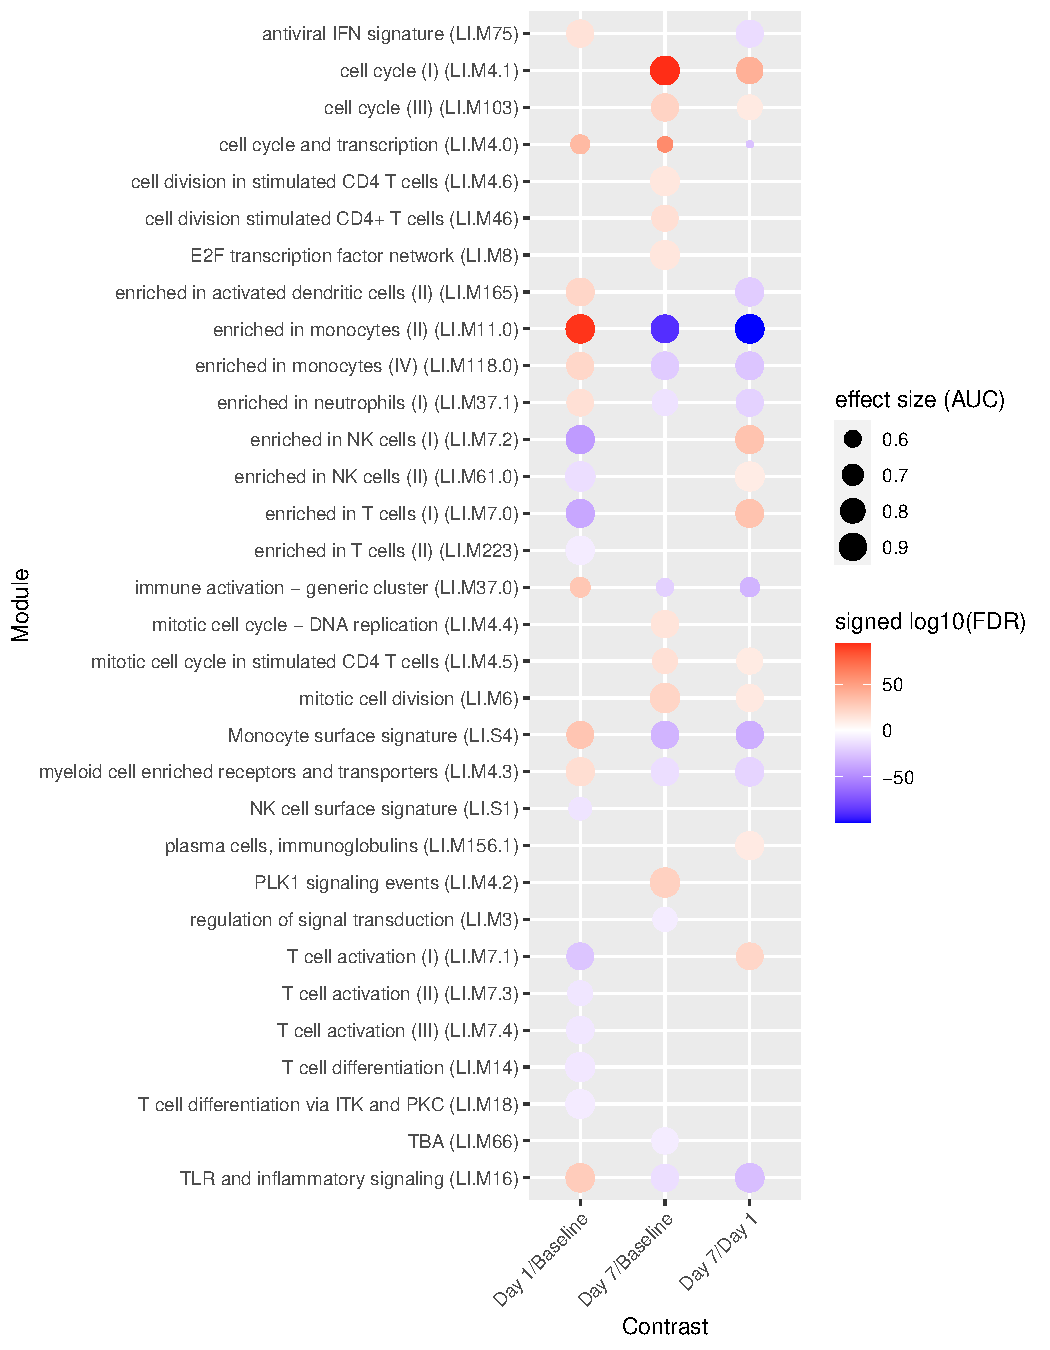
\includegraphics[width=1.0\textwidth]{mainmatter/figures/chapter_02/compare_dge_eqtl.tmodDotPlot.DGE.timepoint.pdf}
    \caption{
        \textbf{Transcriptomic modules up or downregulated between pairs of timepoints.}
        The top ten most significant modules for each contrast are shown.
        Size of circle indicates absolute effect size (\gls{AUC}). 
        Color of circle indicates significance (\gls{FDR} < 0.05) and direction of effect (red = upregulation, blue = downregulation).
        Absence of circle indicates non-significance.
    }
    \label{fig:hird_tmodDotPlot_timepoint}
\end{figure}

\subsubsection{Adaptive immune response at day 7 post-vaccination}
\label{subsec:hird_dge_adaptive_immune_day7}

Fifty-nine genes were differentially expressed at day 7 vs. baseline.
The genes with the highest upregulation were genes associated with B cell differentiation and maturation: \gene{TNFRSF17} (marginal zone B and B1 cell specific protein, $\log_2\text{\gls{FC}} = \num{1.7538617}$) and \gene{MZB1} (B-cell maturation antigen, $\log_2\text{\gls{FC}} = \num{1.7369668}$).
Genes specific to plasma cells, including \gene{SDC1} (which encodes CD138, required for plasma cell maturation \autocite{mccarron2017CD138MediatesSelection}) ($\log_2\text{\gls{FC}} = \num{1.3673081}$) and \gene{ELL2} (which mediates antibody secretion \autocite{martincic2009TranscriptionElongationFactor}) ($\log_2\text{\gls{FC}} = \num{0.8679659}$) were also prominently upregulated.
This matches an almost 5-fold increase in plasma cell abundance at day 7 compared to baseline \autocite{sobolev2016AdjuvantedInfluenzaH1N1Vaccination}.
Strongly enriched modules at day 7 were related to mitosis and cell proliferation, particularly in CD4\textsuperscript{+} T cells (\cref{fig:hird_tmodDotPlot_timepoint}).
Both the CD4\textsuperscript{+} T cell and plasma cell response are indications of a shift toward an adaptive and primarily humoral immune response by day 7.

\subsection{Expression associations with antibody response}

\subsubsection{Detection of gene-level associations was hindered by between-platform heterogeneity}

Using only array expression data, \textcite{sobolev2016AdjuvantedInfluenzaH1N1Vaccination} identified a set of 62 genes with day 7 expression associated with antibody response, 
where response was defined as a binary phenotype based on 4-fold increases in \gls{HAI} or \gls{MN} titres from day -7 to day 63.
Many of these genes were related to plasma cell development and antibody production.
I aimed to find genes similarly associated with antibody response in the meta-analysis of array and \gls{RNAseq} expression data,
and assess the replication of the 58/62 genes that fell into the set of \num{13593} genes measured by both platforms.

I computed a baseline-adjusted, continuous measure of antibody response, the \gls{TRI} \autocite{bucasas2011EarlyPatternsGene}.
The \gls{TRI} is comparable to the binary definition in ranking (\cref{fig:hird_tri}g, \cref{fig:hird_tri}h), but as a continuous phenotype, it improves statistical efficiency to detect associations.
Within just the array data, 51/58 genes were replicated ($\text{\gls{FDR}} < 0.05$), 
confirming \gls{TRI} and the binary response phenotype were comparable.
However, using only the \gls{RNAseq} data replicated 0/58 genes.

In the initial frequentist random-effects meta-analysis,
with a significance threshold of $\text{\gls{FDR}} < 0.05$, 6 genes had expression associated with \gls{TRI} at baseline (\cref{fig:hird_DGE_effectSizeComparisons_rma}f), 55 at day 7 (\cref{fig:hird_DGE_effectSizeComparisons_rma}h), and 11 pooling samples over all timepoints (\cref{fig:hird_DGE_effectSizeComparisons_rma}e).
Of the day 7-specific associations reported by \textcite{sobolev2016AdjuvantedInfluenzaH1N1Vaccination} (circled in \cref{fig:hird_DGE_effectSizeComparisons_rma}h), 
15/58 replicated, all with the same positive direction of effect (high expression with high \gls{TRI}).
However, almost all significant results displayed higher effect sizes in the array compared to \gls{RNAseq} (13/15 genes).
This was in contrast to the associations identified with timepoint, where significant genes had more consistent effects between platforms along the diagonal (\cref{fig:hird_DGE_effectSizeComparisons_rma}b--d).
The likely cause is the presence of more extreme antibody response phenotypes (higher \gls{TRI} range) in the array versus the \gls{RNAseq} dataset (\cref{fig:hird_phenotypes_by_platform}).
This represents an additional source of between-platform variation not due to technical factors, but inherent to the samples themselves.

The Bayesian meta-analysis pipeline more robustly models between-study heterogeneity due to platform and sample-specific effects. 
Due to shrinkage of effects, few genes with effects closer to the dense center of the effect distribution were called as significant, and significant genes tended to have outlying effect sizes in both platforms (compare \cref{fig:hird_DGE_effectSizeComparisons_rma}b--d with \cref{fig:hird_DGE_effectSizeComparisons_bayesmeta}b--d).
No single gene was detected as significantly associated with \gls{TRI} at $\text{\gls{lfsr}} < 0.05$ for any contrast:
not at any single timepoint, nor when pooling samples across all timepoints (\cref{fig:hird_DGE_effectSizeComparisons_bayesmeta}e--h).
The frequentist meta-analysis is likely to use poor estimates of the between-platform heterogeneity, as there are only two data points to estimate it from.
Indeed, all 15 significant genes with day 7 expression associated with \gls{TRI} in the frequentist meta-analysis
had unrealistic between-platform heterogeneity estimates of exactly zero (\cref{fig:hird_DGE_sobolev2016hits_tauComparison}).

\begin{figure}
    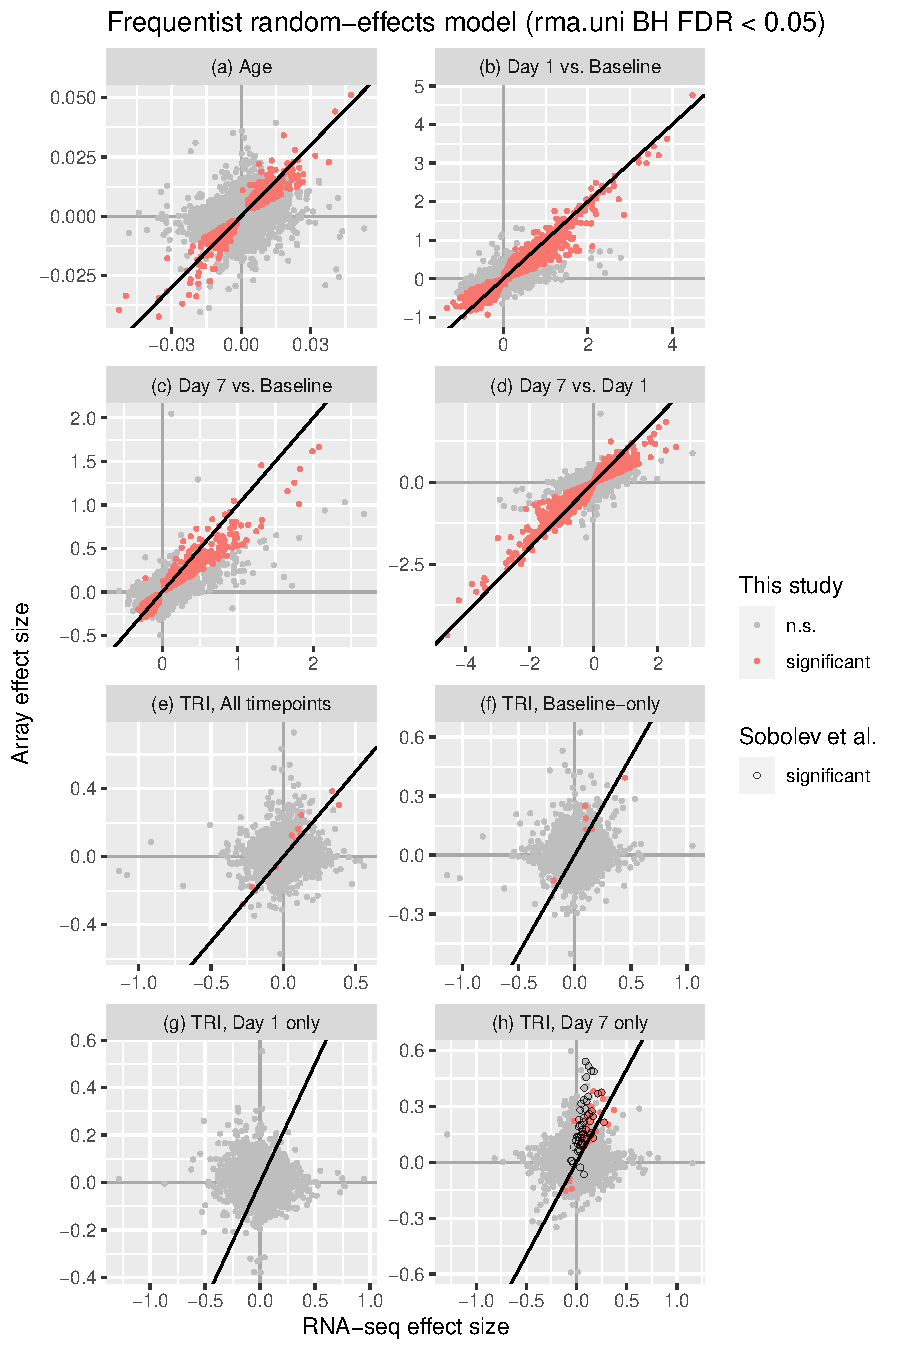
\includegraphics[width=0.9\textwidth,page=1]{mainmatter/figures/chapter_02/plot_dge_eqtl.DGE.effectSizeComparison.pdf}
    \caption{
        \textbf{\gls{DGE} effect sizes ($\log_2\text{\gls{FC}}$) estimated in array versus \gls{RNAseq} samples, colored by significance in frequentist random effects meta-analysis using \software{rma.uni} at $\text{\gls{BH} \gls{FDR}} < 0.05$.}
    Genes with day 7 expression associated with binary responder/non-responder status in \textcite{sobolev2016AdjuvantedInfluenzaH1N1Vaccination} are circled for that contrast.
    }
    \label{fig:hird_DGE_effectSizeComparisons_rma}
\end{figure}

\begin{figure}
    \includegraphics[width=0.9\textwidth,page=2]{mainmatter/figures/chapter_02/plot_dge_eqtl.DGE.effectSizeComparison.pdf}
    \caption{
        \textbf{\gls{DGE} effect sizes ($\log_2\text{\gls{FC}}$) estimated in array versus \gls{RNAseq} samples, colored by significance in Bayesian random effects meta-analysis using \software{bayesmeta} at \software{ashr} $\text{\gls{lfsr}} < 0.05$.}
    Genes with day 7 expression associated with binary responder/non-responder status in \textcite{sobolev2016AdjuvantedInfluenzaH1N1Vaccination} are circled for that contrast.
    }
    \label{fig:hird_DGE_effectSizeComparisons_bayesmeta}
\end{figure}

\begin{figure}
    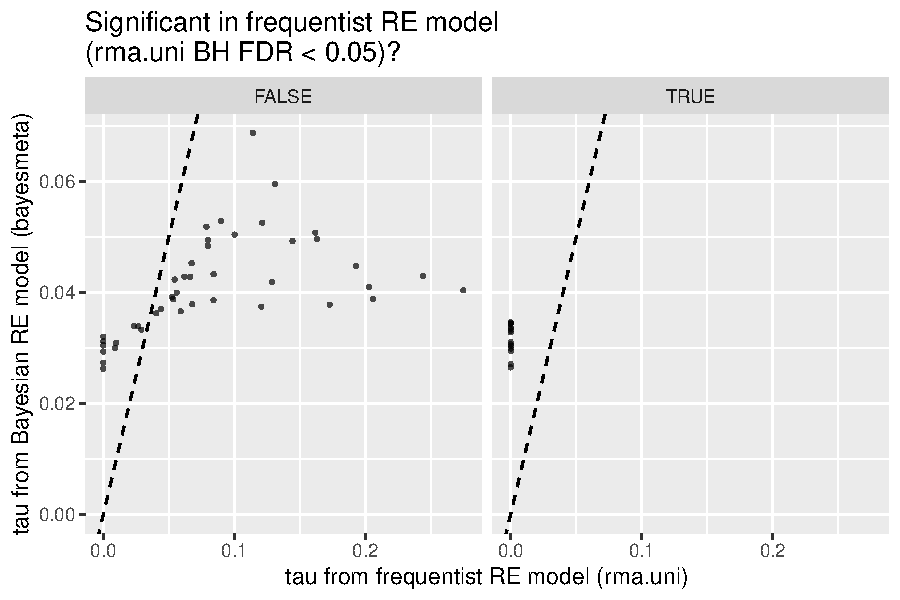
\includegraphics[width=1.0\textwidth,page=1]{mainmatter/figures/chapter_02/plot_dge_eqtl.DGE.sobolev2016_d7R.vs.d7NR.tauComparison.pdf}
    \caption{
        \textbf{Estimates of between-platform heterogeneity $\tau$ from frequentist and Bayesian meta-analysis, for the 58 genes with a significant association between day 7 expression and binary responder/non-responder status in \textcite{sobolev2016AdjuvantedInfluenzaH1N1Vaccination}.}
        Dashed line is the identity line.
        Estimates from the frequentist method cover a wide range and can be zero.
        For this contrast testing association between day 7 expression and \gls{TRI}, \num{8563/13593} of per-gene $\tau$ estimates are zero,
        including all 15/58 significant results (right).
        Significant results are array-driven, with 13/15 having higher effects in array than \gls{RNAseq} (54/58 genes overall).
        Estimates of $\tau$ from the Bayesian method are in a narrower range and constrained away from zero by the prior.
    }
    \label{fig:hird_DGE_sobolev2016hits_tauComparison}
\end{figure}

\subsubsection{Module level associations with antibody response}

Using effect sizes from the Bayesian meta-analysis,
significant enrichments were detectable at the gene set level.
The strongest effects were seen at day 7, where expression of modules related to the cell cycle, CD4\textsuperscript{+} T cells, and plasma cells were positively associated with \gls{TRI}---\enquote{cell cycle (I)} (LI.M4.1, $\text{\gls{FDR}} = \num{6.808113e-54}$),
\enquote{Plasma cell surface signature} (LI.S3, $\text{\gls{FDR}} = \num{1.783164e-12}$),
and \enquote{cell division stimulated CD4+ T cells} (LI.M46, $\text{\gls{FDR}} = \num{5.541366e-10}$) (\cref{fig:hird_tmodDotPlot_TRI}).

Associations with \gls{TRI} were also detected at baseline.
A diverse set of set of modules had positive associations, including
\enquote{chemokines and inflammatory molecules in myeloid cells} (LI.M86.0,  $\text{\gls{FDR}} = \num{2.252190e-11}$),
\enquote{platelet activation - actin binding} (LI.M196, $\text{\gls{FDR}} = \num{1.712211e-08}$),
\enquote{enriched in B cells (I)} (LI.M47.0, $\text{\gls{FDR}} = \num{2.400150e-07}$),
\enquote{cell adhesion} (LI.M51, $\text{\gls{FDR}} = \num{1.216638e-10}$),
\enquote{myeloid, dendritic cell activation via NFkB (I)} (LI.M43.0, $\text{\gls{FDR}} = \num{4.675413e-07}$),
and \enquote{proinflammatory dendritic cell, myeloid cell response} (LI.M86.1, $\text{\gls{FDR}} = \num{4.106130e-07}$).
Monocyte modules 
\enquote{enriched in monocytes (II)} (LI.M11.0, $\text{\gls{FDR}} = \num{3.533733e-04}$) and
\enquote{Monocyte surface signature} (LI.S4, $\text{\gls{FDR}} = \num{1.170804e-03}$)
were negatively association with \gls{TRI}.
Negative associations for these same modules were also maintained at day 1 (LI.M11.0, $\text{\gls{FDR}} = \num{1.407899e-10}$;
LI.S4, $\text{\gls{FDR}} = \num{1.741434e-06}$)
and at day 7 (LI.M11.0, $\text{\gls{FDR}} = \num{5.541366e-10}$) (\cref{fig:hird_tmodDotPlot_TRI}).

\begin{figure}
    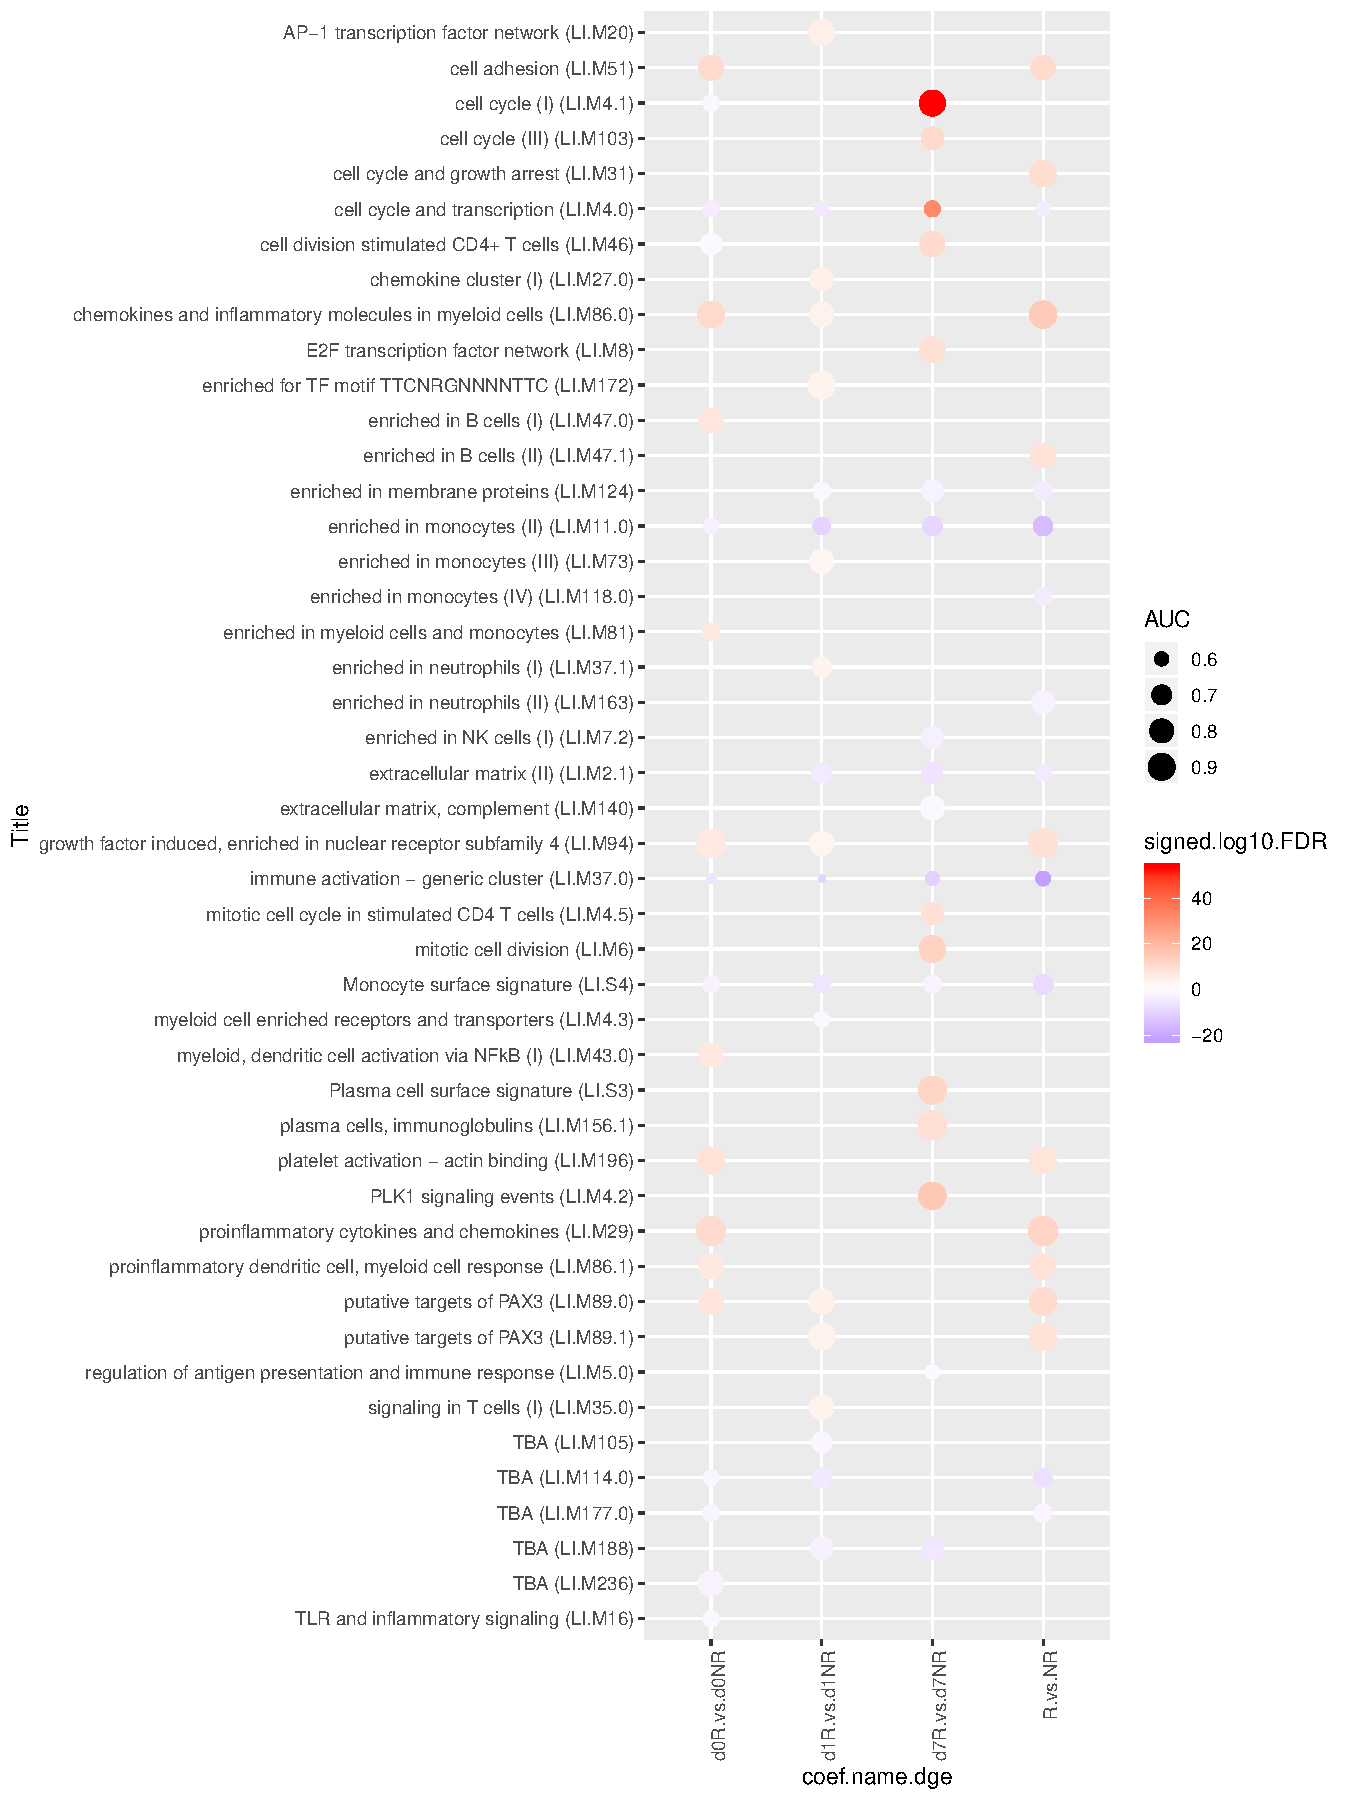
\includegraphics[width=1.0\textwidth]{mainmatter/figures/chapter_02/compare_dge_eqtl.tmodDotPlot.DGE.TRI.pdf}
    \caption{
        \textbf{Gene expression modules associated with antibody response (\gls{TRI}).}
        Enrichments were performed with all timepoints pooled, and at each timepoint specifically.
        The top ten most significant modules for each contrast are shown.
        Size of circle indicates absolute effect size (\gls{AUC}). 
        Color of circle indicates significance ($\text{\gls{FDR}} < 0.05$) and direction of effect (red = expression positively correlated with \gls{TRI}, blue = negatively correlated).
        Absence of circle indicates non-significance.
    }
    \label{fig:hird_tmodDotPlot_TRI}
\end{figure}

\section{Discussion}

A meta-analysis of array and \gls{RNAseq} data revealed extensive transcriptomic response to Pandemrix vaccination in the \gls{HIRD} cohort.
%
At day 1, there was
upregulation of genes and modules related to monocytes, interferon signalling, and the inflammatory response;
and downregulation of T cell and \gls{NK} cell genes and gene modules.
% NOTE: TMM norm guards against composition bias, so up/downregulation between samples is actually valid
Concordant changes in these gene modules were also reported by \textcite{nakaya2016SystemsBiologyImmunity} at day 1 after MF59-adjuvanted seasonal \gls{TIV} in young children, but changes in these modules were not as consistent in children who received non-adjuvanted \gls{TIV}.
The AS03 adjuvant in Pandemrix is thought to act by promoting chemokine secretion, predominantly targeting monocytes and macrophages \autocite{morel2011AdjuvantSystemAS03,wilkins2017AS03MF59AdjuvantedInfluenza}, which concurs with the strong upregulation of monocyte and \gls{DC} modules observed at day 1 after Pandemrix.
A large component of the expression response at day 1 may reflect response to the adjuvant.
%
Most genes differentially expressed at day 1 returned to baseline expression by day 7.
\textcite{nakaya2016SystemsBiologyImmunity} saw a similar trend comparing day 0 and day 3 for MF59-adjuvanted \gls{TIV}.
Unadjuvanted seasonal \gls{TIV} also causes peak transcriptomic induction at day 1 \autocite{bucasas2011EarlyPatternsGene}.
Although the timepoint resolution here is coarse,
the early innate response to Pandemrix is transient, peaking less than 7 days, and likely less than 3 days post-vaccination.
%
Upregulation of cell cycle, proliferating CD4\textsuperscript{+} T cell, and B (plasma) cell genes and modules were detected at day 7.
This indicates a shift to the adaptive immune response, likely involving CD4\textsuperscript{+} T cell-supported differentiation and proliferation of \glspl{ASC}.

Both day 1 and day 7 expression module changes were concordant with changes in cell populations seen in the \gls{HIRD} \gls{FACS} data.
The greater magnitude of expression fold change of individual genes compared to cell abundance fold changes suggests the influence of both mechanisms \autocite{sobolev2016AdjuvantedInfluenzaH1N1Vaccination}.
Statistical adjustment for measured or estimated cell composition is one possibility; I explore these methods in \cref{ch:hird_reQTL} and \cref{ch:multiPANTS}.
An experimental approach would be \textit{in vitro} stimulation of \glspl{PBMC} with vaccine, ruling out cell migration, but not shifts in cell subtype composition \autocite{querec2009SystemsBiologyApproach}.

The overall patterns of expression over time were consistent between array and \gls{RNAseq}, with the meta-analysis identifying genes with outlying effects in both platforms.
In contrast, I was not able to replicate the 58 gene-level associations reported by \textcite{sobolev2016AdjuvantedInfluenzaH1N1Vaccination} between day 7 expression and antibody response that were assessable in my meta-analysis.
The difference was not wholly due to response definitions, as within the array data alone, switching from binary response status to \gls{TRI} still replicated the majority of reported associations,
but using either binary response status or \gls{TRI} in the \gls{RNAseq} data alone found no significant associations.
Initially, 15/58 signals replicated using frequentist random-effects meta-analysis to combine per-platform estimates.
I do not consider these hits as robust, as the estimated between-platform heterogeneity was zero for all 15 of these signals.
None of these signals replicated in the Bayesian random-effects meta-analysis,
where prior information about $\tau$ could be incorporated, discouraging unrealistic estimates of zero heterogeneity.
The Bayesian meta-analysis was in general more conservative, calling fewer differentially expressed genes compared to the frequentist analysis for all contrasts.
Most of the 58 genes also had larger effects in the array dataset than in the \gls{RNAseq} dataset, possibly because the array data contains more extreme \glspl{TRI}.
At a single-gene level, significant associations with timepoint are robustly detectable, 
but associations with \gls{TRI} have effects too modest relative to the noise introduced by platform-dependent technical effects and dataset-dependent phenotype distributions.
%
% Other caveats of the meta analysis
% - The very fact that a meta-analysis is performed adds some bias towards genes with fold changes that can be more consistently measured between platforms; these tend to be genes with higher expression.

Expression associations with antibody response were, however, observed at the gene set level, at modules associated with \gls{TRI} as a whole.
The strongest effects were observed at day 7, where modules related to adaptive immunity (cell cycle, stimulated CD4\textsuperscript{+} cells, plasma cells) were positively associated with \gls{TRI}.
These same modules were upregulated at day 7 compared to baseline; it seems that those individuals with the greatest antibody response to vaccination are most able to induce these modules by day 7 post-vaccination.

Module associations with \gls{TRI} were also observed pre-vaccination with both positive (e.g. chemokines, proinflammatory \glspl{DC}, B cells, platelet activation) and negative (e.g. monocytes) directions of effect, suggesting baseline immune state has influence on long-term antibody response to Pandemrix.
% Over the years, a diverse range of gene sets have been found to be baseline predictors of antibody response to seasonal influenza vaccination:
%     apoptosis \autocite{furman2013ApoptosisOtherImmune};
%     Fc$\gamma$ receptor-mediated phagocytosis, TREM1 signaling \autocite{tsang2014GlobalAnalysesHuman};
%     B cells, T cell activation \autocite{nakaya2015SystemsAnalysisImmunity};
%     B cell receptor signalling, inflammatory response, platelet activation \autocite{hipc-chisignaturesprojectteam2017MulticohortAnalysisReveals};
% several of which I also observe.
Some of the positive associations have been previously reported for unadjuvanted seasonal influenza vaccines in multiple independent cohorts.
The same B cell modules were reported by \textcite{nakaya2015SystemsAnalysisImmunity}, 
and similar \gls{DC}, inflammatory, and platelet activation modules were found to be predictive of antibody response in young adults \autocite{hipc-chisignaturesprojectteam2017MulticohortAnalysisReveals}.
The negative association of monocyte modules with antibody response at baseline was also reported by \textcite{nakaya2015SystemsAnalysisImmunity}.
Interestingly, I detected the same negative associations at day 1 and day 7.
Monocyte modules were one of the most upregulated modules at day 1,
and although the module annotations do not separate monocyte subsets,
abundance of CD16\textsuperscript{+} inflammatory monocytes was particularly increased at day 1 in the \gls{FACS} data \autocite{sobolev2016AdjuvantedInfluenzaH1N1Vaccination}.
This lends some support to the hypothesis that chronic baseline inflammation or excessive/prolonged post-vaccination inflammation---specifically driven by monocytes---can be detrimental to the humoral response \autocite{mitchell2012SuppressionVaccineImmunity,mohanty2015ProlongedProinflammatoryCytokine,nakaya2015SystemsAnalysisImmunity}.

%
% Day 1 TRI ?
% Inflammatory signatures of non-response
% https://www.jacionline.org/article/S0091-6749(17)31766-9/fulltext#sec2.4
% \enquote{The reduced efficacy of vaccination has also been linked to excessive inflammation for influenza,31 yellow fever,32 tuberculosis,33 and hepatitis B34 vaccines.}

There are several caveats to consider when drawing comparisons to the systems vaccinology literature.
Most studies are of unadjuvanted multivalent seasonal vaccines; \gls{HIRD} used an adjuvanted monovalent pandemic vaccine.
Most studies measure post-vaccination antibody response around the expected peak of day 28; \gls{HIRD} measured later at day 63, which may attenuate the signal.
% - the day 63 timepoint is late compared to many other studies
% - Nauta JJ, Beyer WE, Osterhaus AD. On the relationship between mean antibody level, seroprotection and clinical protection from influenza. Biologicals 2009; 37:216-21; PMID:19268607; http://dx. doi.org/10.1016/j.biologicals.2009.02.002 "In clinical studies seroprotection is normally defined as a specific antibody titer or antibody titer increase (seroconversion)."
% - other measures of seroconversion \url{https://www.who.int/biologicals/vaccines/Annex_2_WHO_TRS_963-3.pdf}
% - https://bmcinfectdis.biomedcentral.com/articles/10.1186/s12879-019-4049-5 Seroconversion may not correspond well to protection...
The specific genes within modules driving associations may also differ between studies.
Nevertheless, the ability to observe module-level associations with \gls{TRI} also reported in previous studies with diverse populations, measurement platforms, influenza seasons, and analysis pipelines,
is a stark contrast to difficulty of replicating single-gene associations even within the \gls{HIRD} cohort itself.
When the effect of individual genes on phenotype is expected to be subtle,
module-level analyses are not only more sensitive, but appear to be more generalisable.

The next step is to explore the utility of the identified associations for prediction.
Although I have identified highly significant associations between expression modules and antibody response,
that does not imply the ability to accurately predict response from expression \autocite{tsang2014GlobalAnalysesHuman}---that is, the existence of molecular signatures.
Some exploration can be done within \gls{HIRD} using cross-validation, or by setting aside a subset (e.g. the array data) as a test set,
but having an independent test set is especially important for prediction to guard against overfitting.
Matched expression and antibody data are rare for adjuvanted and pandemic vaccines,
so an initial effort would likely draw on published seasonal vaccine datasets (e.g. \autocite{nakaya2015SystemsAnalysisImmunity,hipc-chisignaturesprojectteam2017MulticohortAnalysisReveals}),
with the aim of identifying shared molecular signatures.

The fundamental question of why gene expression and antibody responses vary between \gls{HIRD} individuals also remains.
Which genes, if their expression were to be modulated, would lead to a change in antibody response?
This is a critical question in the move from identifying correlates of protection and molecular signatures, towards targeted interventions to improve vaccine outcomes \autocite{tsang2020ImprovingVaccineinducedImmunity}.
The descriptive design of the \gls{HIRD} study does not lend itself to exploring causation between expression and antibody titres without a causal anchor.
Interindividual genetic variation could play such a role; \cref{ch:hird_reQTL} will examine the impact of common host genetic variants on expression response in the \gls{HIRD} cohort.

% Beyond Abs: not able to explore actual protectiveness
%
% - Influenza vaccine–induced human bone marrow plasma cells decline within a year after vaccination \url{https://science.sciencemag.org/content/early/2020/08/12/science.aaz8432}
% - Systems immunology: Beyond antibody titers cao2016SystemsImmunologyAntibody

% IFN gamma
%
% Sobolev:
% Of the volunteers analyzed, essentially all showed expansive changes in peripheral blood gene expression by day 1 (significant changes in ~9,000 gene probes (P < 0.05)) (Supplementary Fig. 2a), highly consistent with other studies that did not use adjuvants8,16,24,25.
% [...]
% In that regard, our study shows that the Pandemrix H1N1 vaccine provokes rapid and expansive, yet transient, activation of myeloid cells and effectors, similarly to changes induced by other vaccines, including flu vaccines lacking adjuvant8,13,15–17. However, our study also reveals a pronounced lymphoid contribution to the early phase of the immune response, most evident in the prominent transient upregulation of IFN-γ, which was not apparent in most other virus vaccine studies.
%
% As noted by \autocite{sobolev2016AdjuvantedInfluenzaH1N1Vaccination}, although the day 1 myeloid response was consistent with studies of non-adjuvanted seasonal influenza vaccines (e.g. \autocite{nakaya2011SystemsBiologyVaccination, bucasas2011EarlyPatternsGene, obermoser2013SystemsScaleInteractive}), the presence of interferon gamma-driven responses was unique to \gls{HIRD}.

% Adjuvants
%
% Although it is known that AS03 does induce expression changes related to innate immune response at the injection site (\url{https://www.sciencedirect.com/science/article/pii/S0264410X11000399?via%3Dihub#sec0010}), the mechanism of action is unknown (\url{https://www.frontiersin.org/articles/10.3389/fimmu.2017.01760/full}), and there have been relatively few studies of the effect of AS03 or AS03-adjuvanted vaccines on the \gls{PBMC} immune transcriptome aside from the \autocite{sobolev2016AdjuvantedInfluenzaH1N1Vaccination} study itself.
%
% https://www.sciencedirect.com/science/article/pii/S1879625711000769?via%3Dihub#bib0180
% Their mechanism of action remains incompletely understood, however they may amplify immune responses by enhancing antigen presentation and recruiting inflammatory cells to the area of antigen deposition (reviewed in [36]).
%
% https://link.springer.com/article/10.1007/s10875-010-9490-6
% Immune responses to inactivated influenza virus adjuvanted with a different oil-in-water emulsion, MF59, have recently been described [35, 36]. Although a direct comparison between the adjuvants is complicated by the fact that different methodologies may have been used to measure immune responses, our data indicate that AS03A-adjuvanted influenza vaccines induce strong HI responses and CD4 T-cell frequencies relative to those induced with the MF59-adjuvanted product.
%
% AS03-adjuvanted split-virion influenza A/H5N1 vaccine: (\gene{GBP1}, \gene{IRF1}, and \gene{STAT1}) expressions are up in adjuvanted (\url{https://journals.plos.org/plosone/article?id=10.1371/journal.pone.0167488}), three genes that play a role in interferon and antiviral response.
%
% A study of the MF59-adjuvanted \gls{TIV} \autocite{nakaya2016SystemsBiologyImmunity}
% nakaya2016SystemsBiologyImmunity for MF59 adjuvanted TIV
%

% Seasonal can prime for H1N1
%
% \2 Efficacy, dosing: \enquote{...a single dose of monovalent 2009 H1N1 vaccine was recommended in adults, but young children were recommended to receive 2 doses (reviewed by [3••]). It is likely that a single dose was sufficient to induce immunity in adults because prior exposure to seasonal H1N1 viruses had immunologically primed the population.}
%
% "Seasonal influenza vaccine provides priming for A/H1N1 immunization." \url{https://www.ncbi.nlm.nih.gov/pubmed/20371459}
%
% Demonstration in a mouse model: \url{https://www.ncbi.nlm.nih.gov/pmc/articles/PMC3024675/}
%
% \2 Inclusion of H1N1 strains into seasonal vaccines
% Sobolev sampled in March 2010 to August 2011
% \2 Later cohorts may have recall response to H1N1 from seasonal vaccination
%
